%%%%%%%%%%%%%%%%%%%%%%%%%%%%%%%%%%%%%%%%%%%%%%%%%%%%%%%%%%%%%%%%%%%%%%%%%%% 
% 
% Generic template for TFC/TFM/TFG/Tesis
% 
% By:
% + Javier Macías-Guarasa. 
% Departamento de Electrónica
% Universidad de Alcalá
% + Roberto Barra-Chicote. 
% Departamento de Ingeniería Electrónica
% Universidad Politécnica de Madrid   
% 
% Based on original sources by Roberto Barra, Manuel Ocaña, Jesús Nuevo,
% Pedro Revenga, Fernando Herránz and Noelia Hernández. Thanks a lot to
% all of them, and to the many anonymous contributors found (thanks to
% google) that provided help in setting all this up.
% 
% See also the additionalContributors.txt file to check the name of
% additional contributors to this work.
% 
% If you think you can add pieces of relevant/useful examples,
% improvements, please contact us at (macias@depeca.uah.es)
% 
% You can freely use this template and please contribute with
% comments or suggestions!!!
% 
%%%%%%%%%%%%%%%%%%%%%%%%%%%%%%%%%%%%%%%%%%%%%%%%%%%%%%%%%%%%%%%%%%%%%%%%%%% 

\chapter{Applications in Autonomous Driving}
\label{cha:applications_in_autonomous_driving}

\begin{FraseCelebre}
	\begin{Frase}
		Trabaja duro en silencio, \\
		y deja que tu éxito \\ 
		haga todo el ruido.
	\end{Frase}
	\begin{Fuente}
		Autor original: Frank Ocean
	\end{Fuente}
\end{FraseCelebre}

\section{Introduction}
\label{sec:8_introduction}

% In this chapter we will detail the experiments carried out to assess the performance of our prediction algorithms, both in terms of accuracy and computational resources (time, \acp{FLOP}, parameters) for real-time applications in the field of \ac{AD}. Regarding the proposed methods, we first make use of some well-established tracking metrics to evaluate the behaviour of our physics-based tracking method; then, we follow the validation method proposed by \cite{gutierrez2021validation} to check how integrating HD map information in the prediction pipeline can be determinant to decrease the risk of collision or at least to minimize the impact velocity in an EURO-NCAP based scenario. After that, we study the prediction metrics obtained in the Argoverse 1 \cite{chang2019argoverse} and Argoverse 2 \cite{wilson2023argoverse} Motion Forecasting datasets. 

In this Chapter we detail the experiments carried out to assess the performance of our final proposal, both in terms of accuracy and computational resources (time, Hz) for real-time applications in the field of \ac{AD}. % Regarding the proposed methods, we first make use of some well-established tracking metrics to evaluate the behaviour of our physics-based tracking method; then, we follow the validation method proposed by \cite{gutierrez2021validation} to check how integrating HD map information in the prediction pipeline can be determinant to decrease the risk of collision or at least to minimize the impact velocity in an EURO-NCAP based scenario. After that, we study the prediction metrics obtained in the Argoverse 1 \cite{chang2019argoverse} and Argoverse 2 \cite{wilson2023argoverse} Motion Forecasting datasets.

% Once we have evaluated our different proposals, the best model (including its social and map version) is selected to carry out some challenging applications.

First, we integrate our prediction pipeline in the \acf{DM} layer of our research group and we study its influence when computing the most optimal action for the ego-vehicle, in contrast to reactive proposals where only the past observations or current adversaries positions are required. Experimental results are obtained in the \acf{SMARTS} \cite{SMARTS} framework based on the \ac{SUMO} \cite{Sumo} simulator. This integration of the prediction pipeline and the \ac{DM} layer was published in the following conference paper \cite{gutierrez2023augmented}: "Augmented Reinforcement Learning with Efficient Social-based Motion Prediction for Autonomous Decision-Making", 2023 IEEE 26th International Conference on Intelligent Transportation Systems (ITSC).
	
Second, the prediction pipeline is integrated in the \ac{ADS} of our research group using the \acf{CARLA} \cite{dosovitskiy2017carla} simulator to study the domain adaptation of our prediction model in complex scenarios of the \ac{CARLA} Autonomous Driving Leaderboard \footnote{https://leaderboard.carla.org/}, inspired in the well-established \ac{NHTSA} typology. Since in this thesis we do not focus on the detection stage, and in the different \ac{MP} datasets the agents are assumed to be tracked before feeding the network, for simplicity purposes, we will make use of a simple-yet-powerful concept such us ray-tracing to obtain a realistic \acf{GT} to emulate the input of multi-tracked agents provided by the different datasets. The main reason to use a ray-tracing-based filtering is to get those agents which are within a certain radius with respect to the ego-vehicle and are observed by the rays of the \ac{LiDAR} sensor in such a way a \ac{SOTA} sensor fusion could detect and track that object. By assuming this, we will be able to deploy and validate (since we have the past and future of the scene) our prediction pipeline in the overall architecture in an efficient and isolated way both in simulation or our real-world vehicle.

\section{Predictions for Decision-Making}
\label{sec:8_decision_making}

% https://xindiwu.github.io/data/motion.pdf

The increasing popularity of \acp{ADS} has brought with it significant challenges in ensuring safe and effective decision-making, particularly in complex urban driving scenarios \cite{Yurtsever2019}. \ac{RL} techniques have emerged as a promising solution to address these challenges \cite{Ravi2020}, outperforming ruled-based approaches that usually cannot solve complex situations \cite{Zhu2019}. They enable \acp{ADS} to learn from their interactions with the driving environment, without relying on pre-defined rules. However, \ac{RL}-based approaches still face a number of limitations that can hinder their development, including issues related to state representation. %In recent years, RL has emerged as a promising approach for developing decision-making policies for AVs \cite{Mnih2015}, outperforming ruled-based approaches that usually cannot solve complex situations \cite{Zhu2019}. However, a large number of interactions with the environment are required to obtain the desired policy. This is why other approaches such as imitation learning \cite{SilverHuangEtAl16nature} and inverse RL \cite{Ross2010}, based on human experts' behaviours are also used in the literature. 

A key challenge in \ac{RL}-based \acp{ADS} is the development of effective state representations that can account for the complexity of urban driving scenarios. Unlike in simpler environments, state representations for urban driving must be able to incorporate a wide range of information, including dynamic features of traffic flows and interactions among different agents. Finding ways to effectively encode this information and develop accurate state representations is essential to enabling \ac{RL}-based \acp{ADS} to generalize to various scenarios and make effective driving decisions. Distilling predictive information from scene representations can aid in the development of effective decision-making policies for \acp{ADS}. By better understanding the potential consequences of different driving actions, \ac{RL}-based \acp{ADS} can make more informed decisions that lead to safer and more efficient driving behaviour.

In this application we propose an approach to enhance the efficiency and generalization of \ac{RL}-based \acp{ADS} in urban driving scenarios. Specifically, we introduce the use of a \ac{MP} module to obtain the future positions of the ego-vehicle and the surrounding vehicles (adversaries) in the scenario. These predictions are the input to an \ac{RL}-based \ac{DM} module that executes high-level actions. Our approach is developed using the \ac{PPO} algorithm  \cite{Schulman2017}.  We carry out the evaluation in an unsignalized T-intersection scenario implemented in the \ac{SMARTS} simulator, as shown in Figure \ref{fig:chapter_8_Applications/dm_t-intersection_scenario}, with and without the proposed state representation and provide a comparison with some baseline methods.

\begin{figure}[h]
	\centering
	%\includegraphics[width=0.45\textwidth]{images/teaser.png}
	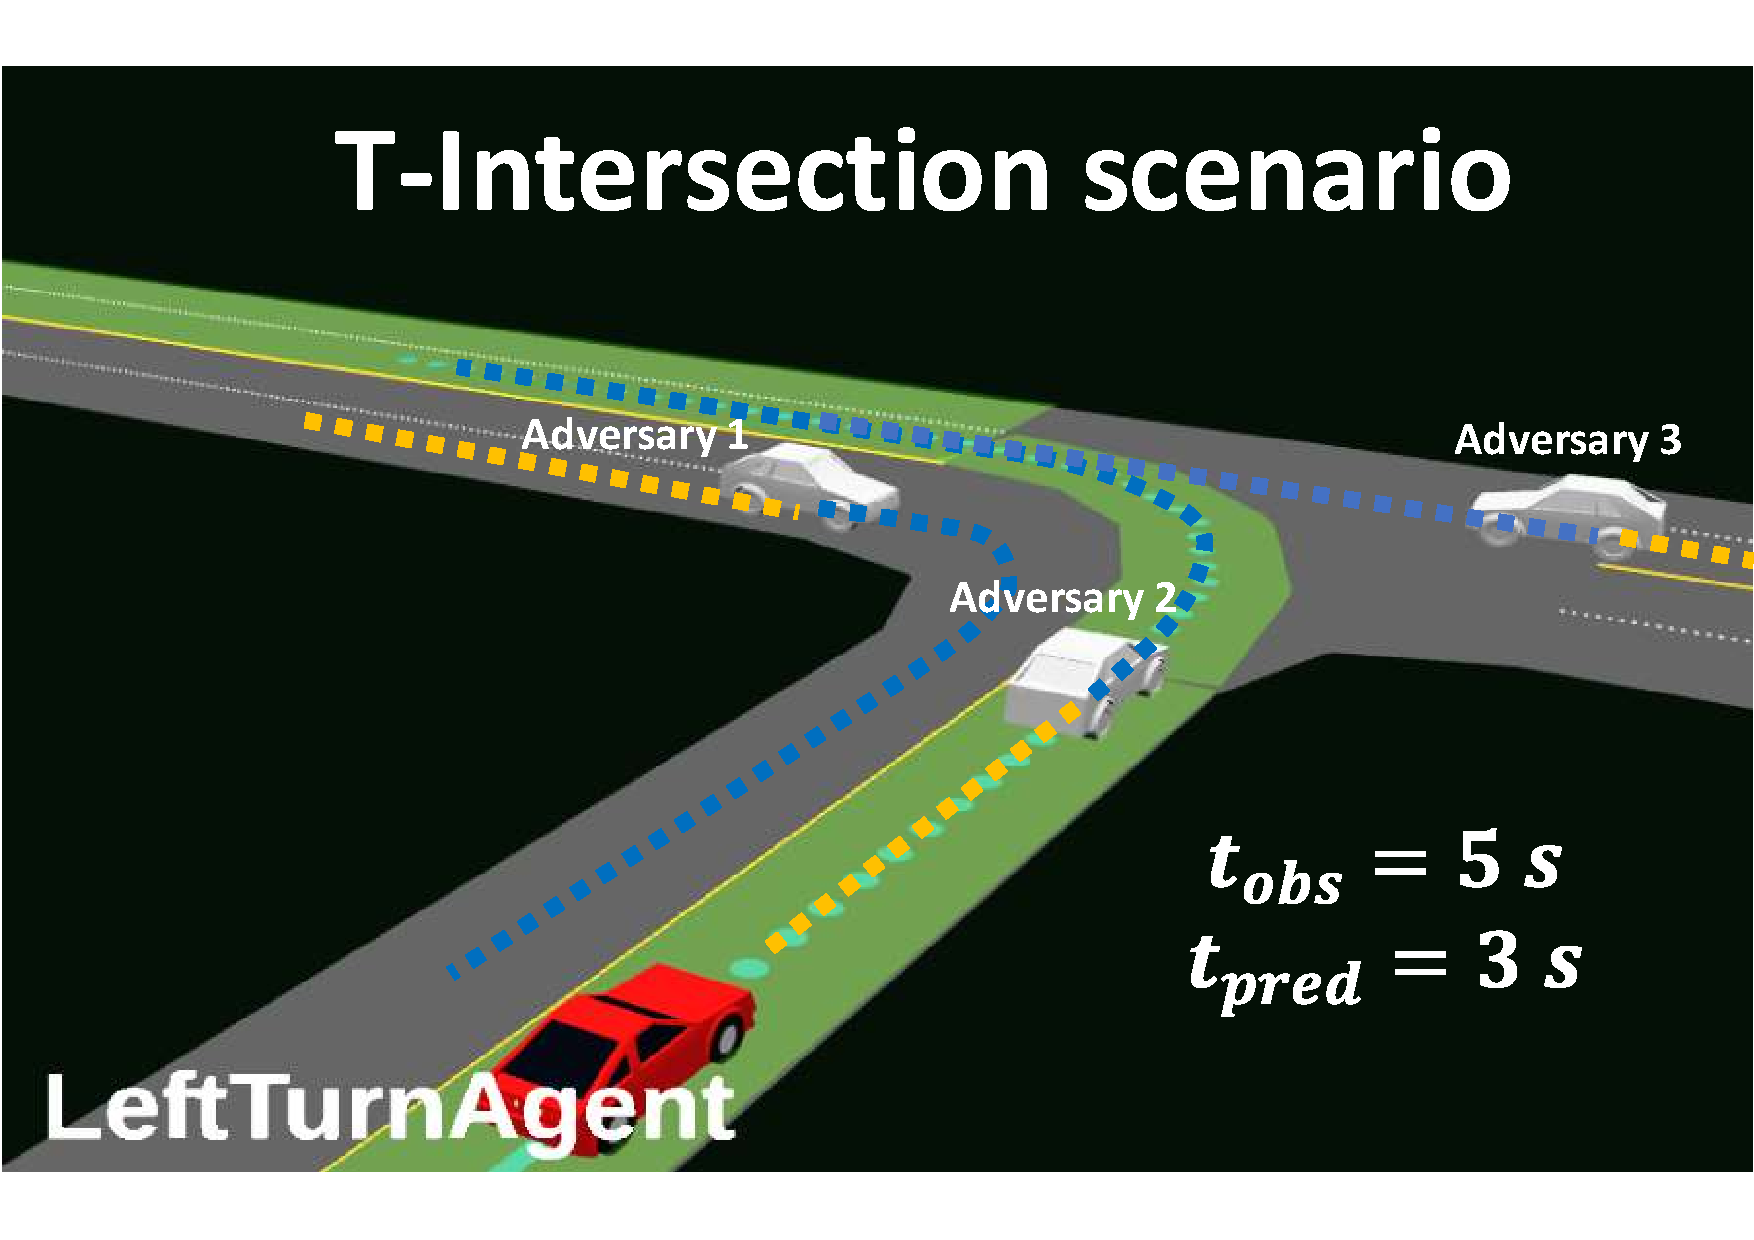
\includegraphics[width=0.45\textwidth]{chapter_8_Applications/dm_t-intersection_scenario.pdf}
	\captionsetup{justification=justified}
	\caption[T-intersection scenario in the \ac{SMARTS} simulator]{T-intersection scenario in the \ac{SMARTS} simulator. The past positions of the adversaries (\textbf{\color{YellowOrange}{yellow}}) and the predicted trajectories (\textbf{\textcolor{blue}{blue}}) are represented in the scenario.}
	\label{fig:chapter_8_Applications/dm_t-intersection_scenario}
\end{figure}

This application is focused on a critical issue for \ac{RL}-based \acp{ADS}, which is the state representation problem. Traditional state representations often focus on low-dimensional features such as distance to obstacles, lane positions, and vehicle velocities \cite{Rodrigo2023}. However, these representations may not be sufficient to capture the complex interactions among different agents and road structures in urban driving scenarios. To address the state representation problem, some methods have been proposed that use high-dimensional or learned representations, such as \acp{CNN} \cite{Johan2018} and \acp{RNN} \cite{Tram2018}; other methods have been proposed to use more detailed representations, such as  \ac{BEV} images \cite{zhang2021endtoend}, image augmentation \cite{kostrikov2021image} or occupancy grids \cite{moghadam2019hierarchical}. These methods have shown promising results in improving the generalization and robustness of the decision-making approaches. Recently, transformer-based approaches have gained increasing attention for their ability to capture long-term dependencies and interactions among different entities in sequential data. In the context of \ac{AD}, transformers have been used to reduce the computational load in end-to-end approaches \cite{Li4} and anticipate future states with prediction-aware planning \cite{valiente2022predictionaware}.

\begin{figure}[h]
	\centering        
	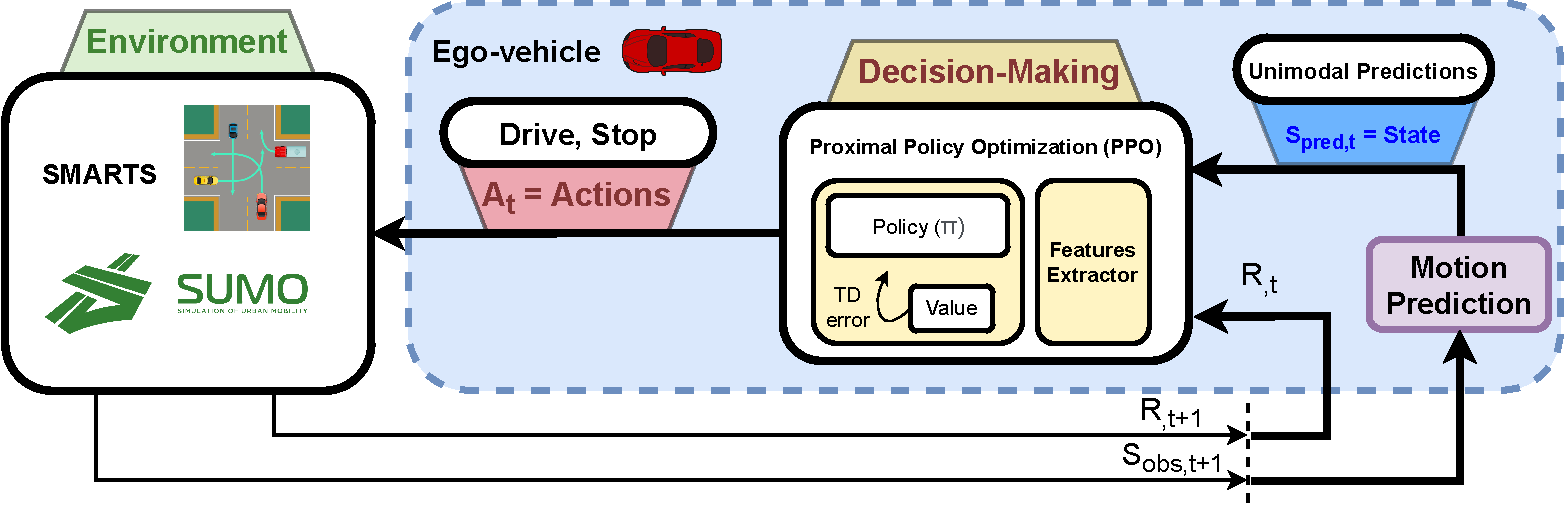
\includegraphics[width=0.95\textwidth]{chapter_8_Applications/dm_prediction_framework.pdf}
	\captionsetup{justification=justified}
	\caption[An overview of the Augmented \ac{RL} with Efficient Social-based \ac{MP} for Autonomous \ac{DM}]{An overview of the Augmented \ac{RL} with Efficient Social-based \ac{MP} for Autonomous \ac{DM}. The observations (both position and ID, so, trackers) of the vehicles in the scenario are obtained from the simulator. The MP module estimates the future positions of these vehicles, taking into account the most plausible score of a multimodal prediction. The decision-making module selects high-level actions based on this information. These actions are executed by the simulator, which provides a new state to the framework.}
	\label{fig:chapter_8_Applications/dm_prediction_framework}
\end{figure}

The objective of this study is to illustrate the efficacy of employing a low-dimensional state representation in conjunction with an MP method. We aim to prove that the proposed framework can lead to good performance in urban scenarios. More specifically, this application presents the following contributions:

\begin{itemize}
	\item The \textbf{augmentation of \ac{RL}-based \ac{DM} techniques with \ac{MP}} to improve state representation. By predicting vehicle trajectories, we can better capture the complex interactions between different agents and road structures in urban driving scenarios. 
	
	\item \textbf{Higher explainability} than end-to-end methods. Intermediate states are accessible in our approach. This can help to understand the decisions made.
	
	\item We provide a \textbf{comparison with baseline methods} in a standard scenario. We demonstrate that our approach leads to some improvements in performance, particularly in scenarios with high velocities.
\end{itemize}

\subsection{Our approach}
\label{subsec:8_decision_making_our_approach}

The \ac{RL} framework proposed in this work, which executes high-level decisions to solve urban driving scenarios, is represented in Figure \ref{fig:chapter_8_Applications/dm_prediction_framework}. The past observations of the position of adversaries are obtained from the environment. This information is provided to our \ac{MP} module (excluding the map for simplicity), which estimates future positions. The \ac{PPO} algorithm takes these predictions and generates the decision-making output.

As observed in Figure \ref{fig:chapter_8_Applications/dm_prediction_framework}, the overall pipeline mainly consists on two different learning processes: supervised learning for the \ac{MP} module and a \ac{RL} approach for the \ac{DM} module. These two modules are trained separately, which allows access to the information of the predictions that feed the \ac{DM} module.

\subsubsection{Efficient Social-based Prediction stage}
\label{subsubsec:8_decision_making_our_approach_prediction}

As observed throughout this thesis, predicting the future behaviour of traffic agents around the ego-vehicle is one of the key unsolved challenges in reaching full self-driving autonomy and it is required to be multi-modal, which means given the past motion of a particular vehicle and its surrounding scene, there may exist more than one possible future behaviour. Therefore, MP models need to cover the different choices a driver could make (\ie \ going straight or turning, accelerations or slowing down) as a possible trajectory in the immediate future or as a probability distribution of the agents future location. In other words, when an \ac{ADS} attempts to make a specific action (\eg \ left turn, brake or accelerate), it must consider the future motion of the other vehicles, since the own future actions (also known as decision-making or behaviour planning) depends on the all possible maneuvers of the other agents of the scene for safe driving. %In our case, though we train the MP model in a multi-modal way, we provide the best mode (trajectory with the highest confidence).

\begin{figure}[h]
	\centering
	\setlength{\tabcolsep}{2.0pt}
	% 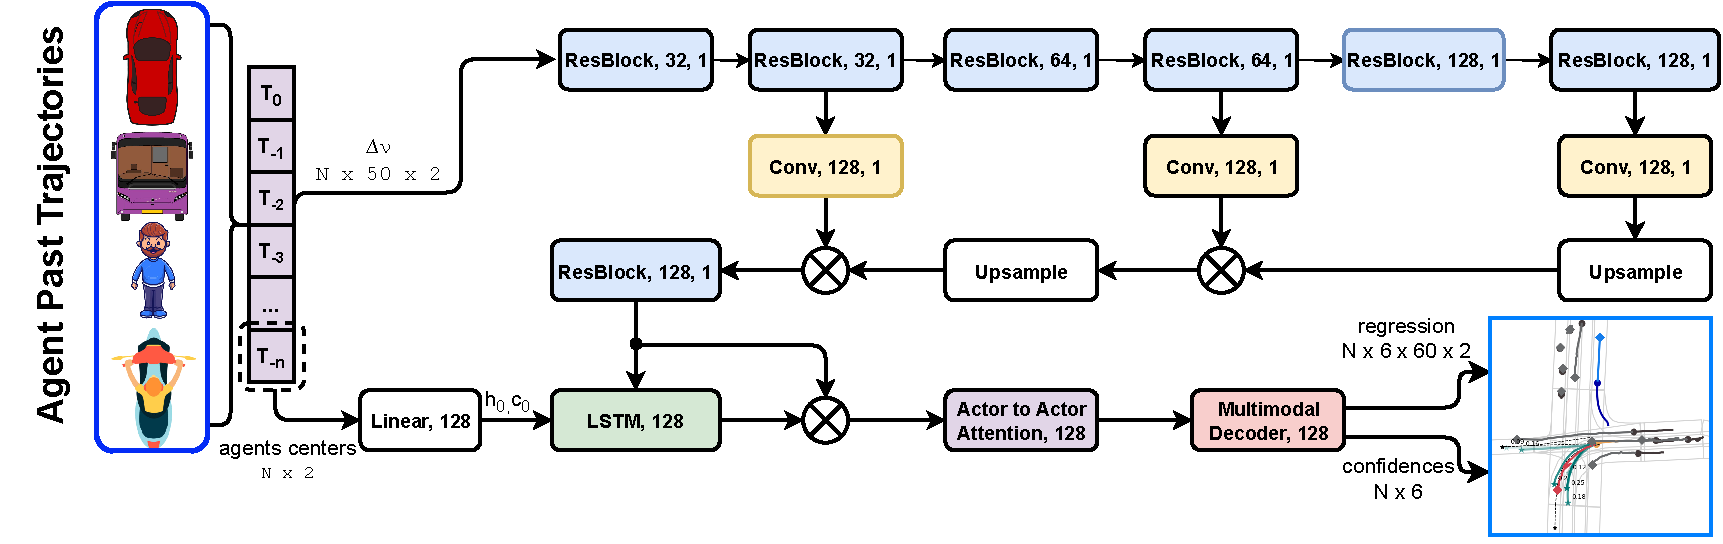
\includegraphics[width=\linewidth]{chapter_8_Applications/social_prediction_baseline.pdf}
	\includegraphics[width=\linewidth]{chapter_8_Applications/CVPR_2023_only_social.pdf}
	\captionsetup{justification=justified}
	\caption[Overview of our Efficient Social-based \ac{MP}]{Overview of our Efficient Social-based \ac{MP}. The main inputs are the relative displacements and centers (last observations) of the agents in the ego-vehicle frame. The relative displacements, agents centers and additional metadata are encoded through a transformer encoder and interactions are computed by means of a Crystal-\ac{GCN}. Finally, \textit{K} final future trajectories (modes) and their confidence scores are computed and refined through a multi-modal decoder and motion refinement module respectively.}
	
	% On the other hand, the agents centers are encoded through a linear layer to initialize the hidden and cell vector of the LSTM layer, which processes the previously latent motion history
	\label{fig:chapter_8_Applications/CVPR_2023_only_social}
\end{figure}

Since our proposed decision-making and \ac{MP} pipeline (Figure \ref{fig:chapter_8_Applications/dm_prediction_framework}) is multi-stage to provide a more interpretable framework, we follow the principles of the Argoverse 2 Motion Forecasting dataset \cite{wilson2023argoverse}. In particular, we take the final proposal of this thesis (Chapter \ref{cha:improving_multi_agent}) but excluding the map and heuristic lane proposals for simplicity. Then, this model is solely based on past trajectories (motion history, $obs_{len} = 50$) and agent metadata (in \ac{SMARTS} we assume all agents are vehicles and are relevant), as observed in Figure \ref{fig:chapter_8_Applications/CVPR_2023_only_social}, which output is a set of multi-modal predictions with $pred_{len} = 60$ future steps.

% CONTINUARRRRRRRRRRRRRRR

The \acf{SMARTS} \cite{SMARTS} framework provides only the positions of the agents in the timestamp \textit{t}. Nevertheless, in order to predict the future $pred_{len}$ trajectories of the agents, we require their corresponding $obs_{len}$ trackers over a certain set of observations. Most vehicle prediction datasets \cite{wilson2023argoverse} aim to predict the future behaviour of a target agent assuming the surrounding agents have been detected and tracked (so, monitored over time) and the map information is also provided. In that sense, since \ac{SMARTS} provide the agents in the same order for consecutive timestamps (that is, the agent 5, unless it disappears from the scene, will be the agent 5 again in the next frame), we are able to compute a FIFO (\textit{First Input First Output}) for each agent, not requiring data association \cite{kuhn1955hungarian} to perform this task. 

On top of that, as proposed by multiple methods \cite{liang2020learning, gomez2023improving}, we consider only the vehicles that are observable at \textit{t=0}, handling those agents that are not observed over the full sequence spectrum (observation length = \textit{$obs_{len}$} + prediction length = \textit{$pred_{len}$}) by concatenating a binary flag $b_i^t$ that indicates if the agent is padded or not. In particular, we filter the static elements and track fragments scored by Argoverse 2 to get only the most relevant traffic agents, reducing the number of agents to be considered in complex traffic scenarios. Furthermore, to make the model translation and rotation invariant, the coordinate system in our model is \ac{BEV}-centered of a given target agent at $t = 0$, and we use the orientation from the target location given in the same timestamp as the positive $x$-axis. Note that this representation will benefit the model to have a common representation to enhance the generalization of the model and prevent overfitting. Once the scene has been translated and rotated, instead of using absolute 2D-\ac{BEV} (\textit{xy} plane), the input for the agent \textit{i} is a series of relative displacements, as stated throughout this thesis.

Then, as stated in Chapter \ref{cha:improving_multi_agent}, we concatenate the agents past trajectories and additional social metadata in order to be processed by a linear embedding. Then, positional encoding is added to the output embedding explicitly to retain the information regarding the order of past trajectories and future preliminar steps. Finally, these latent features feed the transformer encoder, leveraging the self-attention mechanism and positional encoding to learn complex and dynamic patterns from long-term time series data. Once we have the latent vector of the different agents, as observed in Figure \ref{fig:chapter_8_Applications/CVPR_2023_only_social}, we learn complex agent-agent interactions by means of a Crystal-\ac{GCN}, which output is finally introduced into the multi-modal decoder. Taking the final actor features after motion history and agents interaction, a multi-modal prediction header outputs the final motion forecasting. For each agent, it predicts $K$ possible future trajectories and their confidence scores. The header has two branches, a regression branch to predict the trajectory of each mode and a classification branch to predict the confidence score of each mode.

For the $m$-th actor, a residual block and a linear layer in the regression branch to regress the $K$ sequences of BEV coordinates is obtained:

\begin{equation}
	O_{m, \text{reg}} = \{ (\mathbf{p}_{m,1}^k, \mathbf{p}_{m,2}^k, ..., \mathbf{p}_{m,T}^k) \}_{k \in [0, K-1]}
\end{equation}

where $O_{m, \text{reg}}$ is the whole set of regressions and $\mathbf{p}_{m,i}^k$ is the predicted $m$-th actor's BEV coordinates of the $k$-th mode at the $i$-th time step.

On the other hand, for the classification branch, a MLP to $\mathbf{p}_{m,T}^k - \mathbf{p}_{m,0}$ to get $K$ distance embeddings is applied. Finally, each distance embedding is concatenated with the actor feature, applying a residual block and a linear layer to output $K$ confidence scores, $O_{m, \text{cls}} = (c_{m,0}, c_{m,1}, ..., c_{m,K-1})$.

Finally, as stated in Chapter \ref{cha:improving_multi_agent}, a motion refinement modules takes into account the preliminary multi-modal predictions computed by the decoder, latent vector before the decoder and past trajectories (including the corresponding meta-data) to fine-tune the final trajectories by means of a regression and orientation loss.

\begin{comment}
Since our model focus on an efficient encoding of the social information, we base our model on the ActorNet backbone proposed by \cite{liang2020learning}, as observed in Figure \ref{fig:chapter_8_Applications/CVPR_2023_only_social}. While both CNNs and RNNs can be used for temporal data, ActorNet uses an 1D CNN to process the trajectory input for its effectiveness in extracting multi-scale features and efficiency in parallel computing. The output is a temporal feature map, whose element at $t=0$ is used as the actor feature. The network has $3$ groups/scales of 1D convolutions. Each group consists of $2$ residual blocks, with the stride of the first block as $2$. Then, a Feature Pyramid Network (FPN) \cite{lin2017feature} is used to fuse the multi-scale features, and apply another residual block to obtain the output tensor. For all layers, the convolution kernel size is $3$ and the number of output channels is $128$. Layer normalization and the Rectified Linear Unit (ReLU) are used after each convolution. 

On top of that, in a similar way to \cite{wang2022ganet}, the agents centers (observations at $t=0$) are encoded through a linear layer to initialize the hidden and cell vector of the LSTM layer, which processes the previously latent motion history. After that, a social attention block is used to compute the most representative agents interaction.

Taking the final actor features after motion history and agents interaction, a multi-modal prediction header outputs the final motion forecasting. For each agent, it predicts $K$ possible future trajectories and their confidence scores. The header has two branches, a regression branch to predict the trajectory of each mode and a classification branch to predict the confidence score of each mode.

For the $m$-th actor, a residual block and a linear layer in the regression branch to regress the $K$ sequences of BEV coordinates is obtained:

\begin{equation}
	O_{m, \text{reg}} = \{ (\mathbf{p}_{m,1}^k, \mathbf{p}_{m,2}^k, ..., \mathbf{p}_{m,T}^k) \}_{k \in [0, K-1]}
\end{equation}

where $O_{m, \text{reg}}$ is the whole set of regressions and $\mathbf{p}_{m,i}^k$ is the predicted $m$-th actor's BEV coordinates of the $k$-th mode at the $i$-th time step.

On the other hand, for the classification branch, a MLP to $\mathbf{p}_{m,T}^k - \mathbf{p}_{m,0}$ to get $K$ distance embeddings is applied. Finally, each distance embedding is concatenated with the actor feature, applying a residual block and a linear layer to output $K$ confidence scores, $O_{m, \text{cls}} = (c_{m,0}, c_{m,1}, ..., c_{m,K-1})$.
\end{comment}

On top of that, in this particular application in the \ac{SMARTS} simulator, we take the most plausible future trajectory for each agent (both the adversaries and the ego-vehicle) in the following timestamps: \textit{t=0}, \textit{t=10}, \textit{t=20} and \textit{t=30}, which correspond to the current position and the predicted position of the corresponding agent 1, 2 and 3 seconds in the future respectively. Even though we train our prediction model following the principles of Argoverse 2 (5s and 6s of observation and prediction respectively), given the velocities and traffic density of the experiments run in the \ac{SMARTS} simulator , we believe that predicting 3s in the future is enough for this purpose to evaluate the high-level actions of decision-making layer preventing over-fitting. In future works, we will design more difficult scenarios, up-to-pair with the Argoverse 2 dataset (specially in terms of intersections or lane change behaviours at high speed) where multi-modal predictions with higher prediction horizons will be required.

\subsubsection{Reinforcement Learning-based Decision Making}
\label{subsubsec:8_decision_making_our_approach_dm}

A \ac{MDP} is a discrete-time stochastic control process that provides a mathematical framework for modelling decision-making environments. An \ac{MDP} is a tuple $(S,A,P,R)$ in which $S$ is a set of states named state space, $A$ is a set of actions named action space, $P$ is the probability function and $R$ is a reward function. An algorithm with a given state $s \in S$ takes an action $a \in A$ transitioning to $s'$ with a probability $P(s,a,s')$, and getting a reward $R(s,a,s')$ as shown in Figure \ref{fig:chapter_8_Applications/dm_prediction_framework}. This algorithm iterates through this loop to learn a desired behaviour. 

The goal in an \ac{MDP} is to find a good policy for the decision-making system. The objective is to find the optimal policy $\pi*(s)$, that maximizes the cumulative function of the future reward.

We represent the driving scenario as an \ac{MDP} to develop our decision-making module. We consider the output of the MP module as an input to this module. The state space, action space, and reward functions are defined in this section.

\paragraph{State space}
\label{par:8_decision_making_our_approach_dm_state_space}

The state is defined by the predicted trajectories of the ego-vehicle and the five closest vehicles in the scenario.

\begin{equation}
	s_t = (K^{ego}_t, K^1_t, ..., K^{5}_t)
	\label{eq:state}
\end{equation}

where $K^{i}_t = (x^i_{t_0}, y^i_{t_0}, x^i_{t_1}, y^i_{t_1}, x^i_{t_2}, y^i_{t_2}, x^i_{t_3}, y^i_{t_3})$ contains the future estimations of the positions of the vehicles across a future horizon of three seconds. A representation of a state vector is shown in Figure \ref{fig:chapter_8_Applications/dm_state}, where the vehicles predicted positions are represented.

\begin{figure}[h]
	\centering
	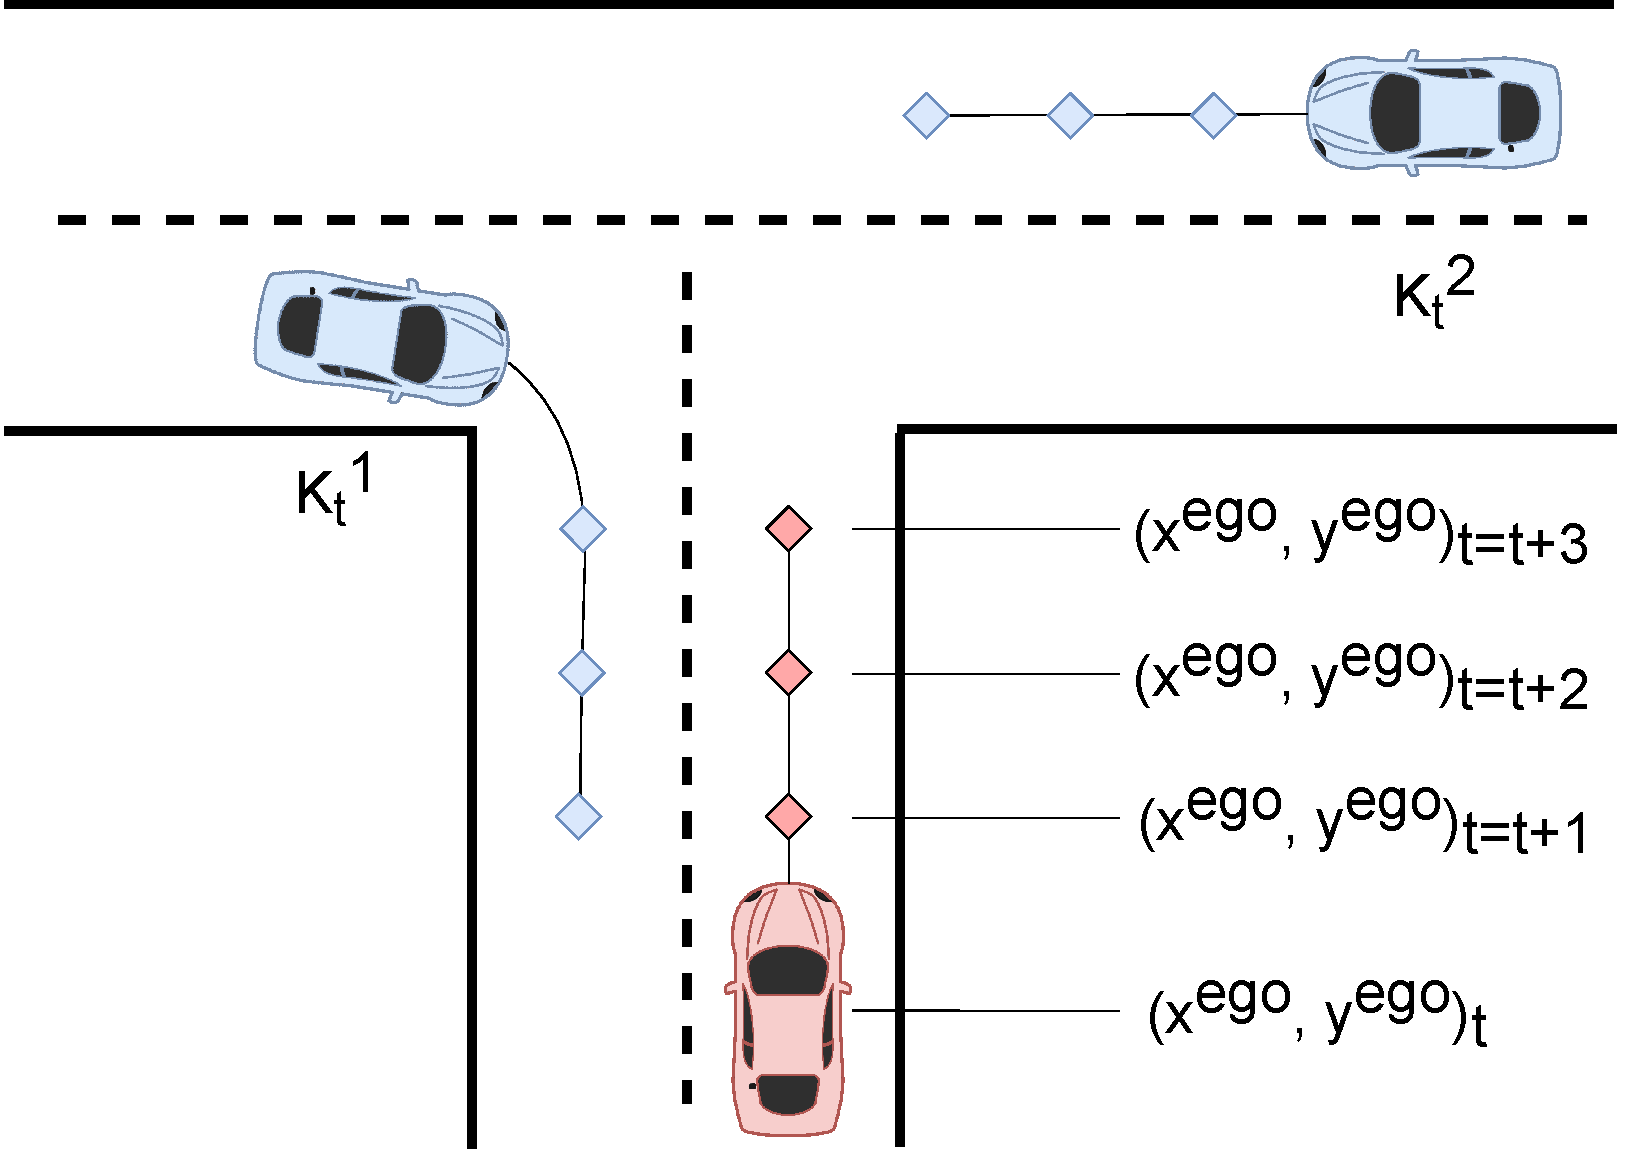
\includegraphics[width=0.40\textwidth]{chapter_8_Applications/dm_state.pdf}
	\caption[Predicted positions of the ego-vehicle and the adversaries in the next 3s]{Predicted positions of the \textbf{\textcolor{red}{ego-vehicle}} and the \textbf{\textcolor{blue}{adversaries}} in the next 3s.}	
	\label{fig:chapter_8_Applications/dm_state}
\end{figure}

\paragraph{Action space}
\label{par:8_decision_making_our_approach_dm_action_space}

We propose a discrete action space formed by two actions. A low-level controller implemented by the simulator is in charge of performing smooth driving based on these actions. These actions are focused on the ego-vehicle velocity. The first action aims to reach a desired predefined velocity and the second action reduces the velocity until the vehicle stops. The action space is defined as:

\begin{equation}
	a=(Drive, Stop)    
	\label{eq:action}
\end{equation}

\paragraph{Reward function}
\label{par:8_decision_making_our_approach_dm_reward_function}

The reward function is defined in terms of success or failure. A negative reward is given when there is a collision and a positive reward is given when the vehicle reaches the success point, situated at the end of the scenario.

\begin{equation}
	r = k_v * v_{ego} + \left\lbrace\begin{array}{lcc}
		1 & if & sucess \\ 
		-1 & if & collision \\
	\end{array}\right.
	\label{eq:Reward}
\end{equation}

As shown in Equation \ref{eq:Reward}, we add one more factor to the reward function to encourage the ego-vehicle to move. We propose a cumulative reward based on its longitudinal velocity. We use a constant small enough to ensure that the reward per episode is bounded between -1 and 1.

Our approach for the RL implementation (Figure \ref{fig:chapter_8_Applications/dm_RL_network}) builds upon our previous research \cite{Gutierrez2022}, where we demonstrated that incorporating a feature extractor module to a \ac{PPO} algorithm yields improved metrics and faster convergence. 

\begin{figure}[h]
	\centering
	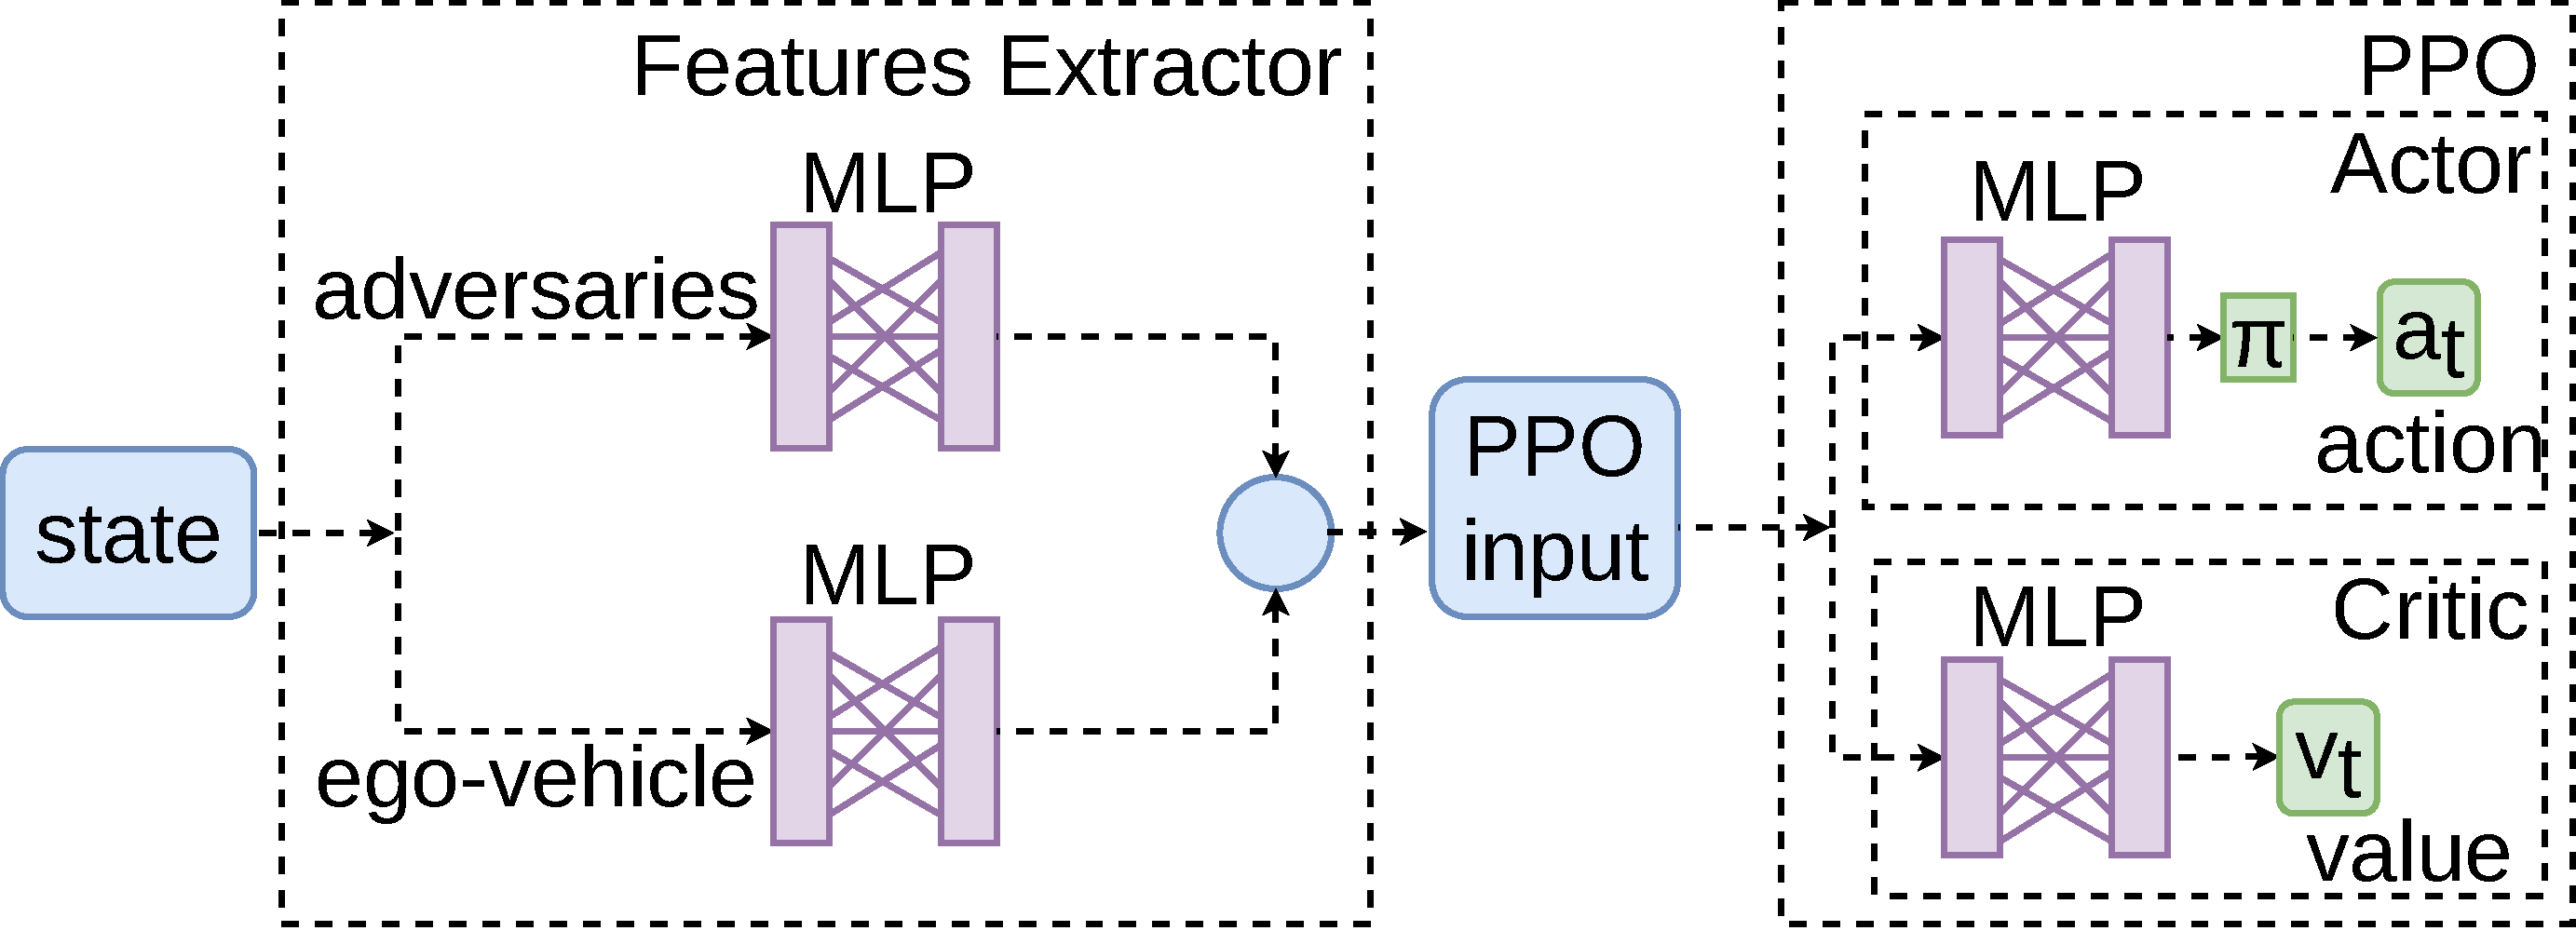
\includegraphics[width=0.8\textwidth]{chapter_8_Applications/dm_RL_network.pdf}
	\captionsetup{justification=justified}
	\caption[Overview of our Reinforcement Learning-based Decision-Making architecture]{Overview of our Reinforcement Learning-based Decision-Making architecture. The neural network architecture consists of two fully connected layers followed by the concatenation of both adversaries and ego vehicle features. The resulting concatenated features are then passed through an actor-critic structure, which comprises two layers, each containing 128 neurons.}	
	\label{fig:chapter_8_Applications/dm_RL_network}
\end{figure}

In this implementation, we introduce separate feature extractors for adversaries and the ego-vehicle, which are then concatenated into the input for the \ac{PPO} algorithm. This algorithm consists of two models: the Actor, responsible for selecting an action based on the policy, and the Critic, which estimates the value function.

\subsection{Experimental results}
\label{subsec:8_decision_making_experimental_results}

\subsubsection{Driving scenario}
\label{subsubsec:8_decision_making_experimental_results_driving_scenario}

To validate the performance of our approach, an intersection scenario is implemented in \ac{SMARTS}, which is a SUMO \cite{Sumo} based simulation platform for research on autonomous driving.

\begin{figure}[h]
	\centering        
	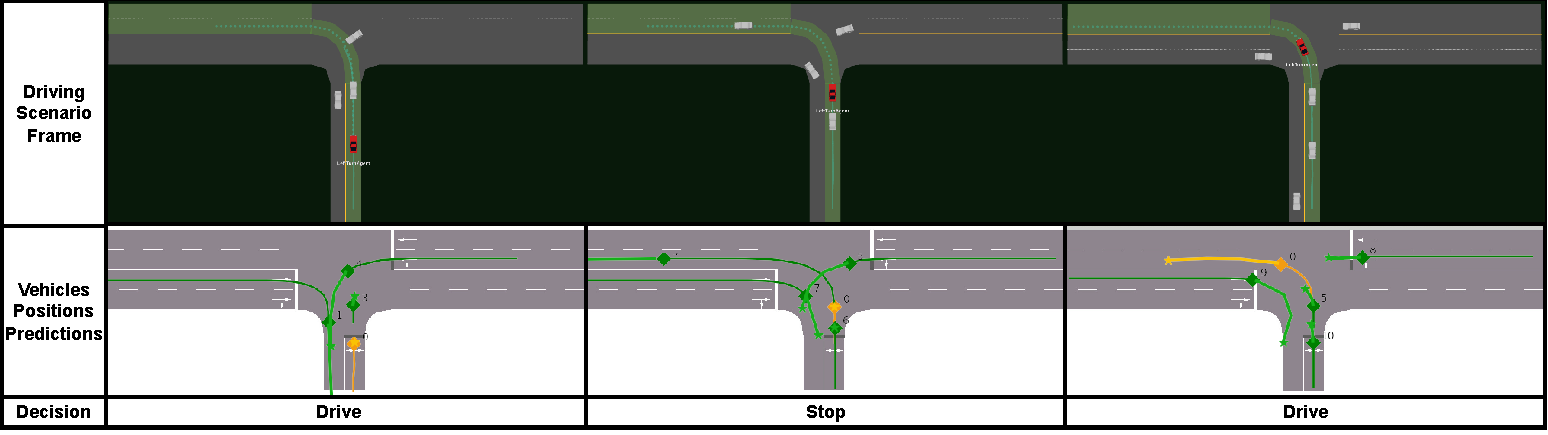
\includegraphics[width=0.95\textwidth]{chapter_8_Applications/dm_prediction_results.pdf}
	\captionsetup{justification=justified}
	\caption[Simulation overview of our system behaviour]{Simulation overview of our system behaviour. The red car follows the green path, and each image represents a different frame of the simulation. We also show the predicted positions below each image and the actions taken by the decision-making module.}
	\label{fig:chapter_8_Applications/dm_prediction_results}
\end{figure}

The scenario is an urban unsignalized T-intersection. The objective is to execute a left turn maneuver in the absence of traffic signal protection, allowing the continuous flow of traffic. Fig. \ref{fig:chapter_8_Applications/dm_t-intersection_scenario} illustrates the drivable area (highlighted in green) where the ego-vehicle can navigate to reach the target location. Simulations are reset under three conditions: 1) the ego-vehicle successfully reaches the target, 2) the episodic step surpasses the maximum time steps limit, and 3) the ego-vehicle collides or deviates from the drivable route.

We define different scenario configurations to test the performance of the proposed framework. First, the regular T-intersection scenario which is defined in \ac{SMARTS}, where a random number of vehicles between [5-10] are spawned every minute, and the maximum velocity of these vehicles is 14 km/h. Then, we propose different configurations increasing the maximum velocity of the adversaries to 30, 60, and 90 km/h. 

\subsubsection{Evaluation Metrics}
\label{subsubsec:8_decision_making_experimental_results_evaluation_metrics}

In decision-making, the success rate serves as a direct measure of the effectiveness of the RL agent in accomplishing the designated task. Besides, the average time of the episode is a common metric used in the literature. These metrics are defined as:

\begin{equation}
	success [\%] = \frac{n_{success}}{n_{episodes}}
\end{equation}

\begin{equation}
	t_{e} [s] = \sum{\frac{t_n}{n_{episodes}}}
\end{equation}

where the number of episodes $n_{e}$ is 100 and simulation time is measured in seconds. 

\subsubsection{Results}
\label{subsubsec:8_decision_making_experimental_results_results}

To evaluate the performance of our approach we first present a comparison with the existing methods for decision-making in the literature and then an ablation study is conducted. 

This first study compares the proposed approach with other existing methods for decision-making. The baseline methods used for comparison are Data-regularized Q-learning (DrQ) \cite{kostrikov2021image}, Soft Actor-Critic (SAC) \cite{haarnoja2019soft}, and PPO. These methods have different features and serve as reference points for evaluating the proposed approach. The results presented in Table \ref{table:comp} demonstrate a higher success rate of our proposal.

\begin{table}[h!]
	\centering
	\captionsetup{justification=justified}
	\caption[Comparison of the proposed framework against the existing baselines in the T-intersection scenario]{Comparison of the proposed framework against the existing baselines in the T-intersection scenario. The success rate S[\%] and the average episode time $t_{e}$ are presented.}
	\label{table:comp}
	%\setlength{\extrarowheight}{2pt}
	\begin{tabular}{c|ccccc} 
		% \ChangeRT{1pt}
		\toprule
		Metric & Ours & PPO & SAC & DrQ \\
		\midrule
		S[\%] & \textbf{80} & 70 & 68 & 78 \\ 
		$t_{e}$(s) & 22.3 & 36.4 & 19.2 & \textbf{18.2} \\
		\bottomrule
		\ChangeRT{1pt}
	\end{tabular}
\end{table}

Two ablative studies are carried out to see how the use of motion prediction in the state representation can improve the performance of the framework. The first approach is to use just the position of the vehicles as the input to the decision-making module and the second approach is to use the locations over the past five seconds. We test the three approaches under the previously introduced configurations with different adversaries' velocities, from 15km/h to 90km/h. To correctly evaluate the performance of the decision-making system we propose different metrics that aim to provide a better comprehension of the behaviour. We believe that the success rate is still a good indicator, but we slightly modify the average time, only considering the successful episodes to calculate this metric. In addition, we include a new relevant metric: the average ego-vehicle velocity when a collision takes place $v_{c}$.  

The results presented in Table \ref{table:chapter_8_Applications/dm_ablation_study_smarts} show that the use of the predicted positions in the state vector avoids more collisions as the velocities increase. Besides, the average collision velocity and the average time to complete the scenario are lower for the proposed approach. 

\begin{table}[h]
	\centering
	\captionsetup{justification=justified}
	\caption[Ablation study comparing three state representations with different scenario configurations]{Ablation study comparing three state representations with different scenario configurations: Current positions, Past positions, and Future positions. The success rate S[\%], the episode time $t_{e}$ in these successful episodes, and the average velocity of collision $v_{c}$ are presented.}
	\label{table:chapter_8_Applications/dm_ablation_study_smarts}
	\setlength{\extrarowheight}{2pt}
	\begin{tabular}{cccccc} 
		\ChangeRT{1pt}
		& Metric & 15 km/h & 30 km/h & 60 km/h & 90 km/h  \\
		\hline 
		\multirow{3}{*}{Future}
		&S [\%] & 80 & 78 & 78 & 77 \\ 
		&$t_{e}$ (s) & 22.3 & 23.3 & 23.4 & 23.3 \\
		&$v_{c}$ (km/h) & 4.9 & 5.1 & 5.6 & 5.6 \\
		\hline
		\multirow{3}{*}{Current}
		&S [\%] & 77 & 73 & 70 & 70 \\ 
		&$t_{e}$ (s) & 25.1 & 23.4 & 23.4 & 23.3 \\
		&$v_{c}$ (km/h) & 5.1 & 5.5 & 6.1 & 6.2 \\
		\hline
		\multirow{3}{*}{Past}
		&S [\%] & 78 & 75 & 72 & 71 \\ 
		&$t_{e}$ (s) & 24.2 & 23.3 & 23.2 & 23.1 \\
		&$v_{c}$ (km/h) & 4.9 & 5.2 & 5.9 & 6.0 \\
		\hline
		\ChangeRT{1pt}
	\end{tabular}
\end{table}

Finally, an overview of the behaviour of our system is shown in Figure \ref{fig:chapter_8_Applications/dm_prediction_results}. The ego-vehicle in red follows the trajectory defined in green. Each image represents a different frame of the simulation and the respective predictions of the positions are displayed below. Besides, the action executed by the decision-making module for each frame is shown.

\section{Domain Adaptation in CARLA simulator}
\label{sec:8_domain_adaptation_carla}

In this Section we study the domain adaptation of our efficient social-based prediction model (Figure \ref{fig:chapter_8_Applications/CVPR_2023_only_social}) in the \ac{CARLA} simulator. As stated in previous sections, \ac{CARLA} provides a realistic sensor simulation environment, including cameras, \ac{LiDAR}, and other on-board sensors. On top of that, it accurately models vehicle dynamics, including realistic acceleration, braking, and steering behaviors in complex traffic scenarios with various types of vehicles, pedestrians, and cyclists, enabling motion prediction algorithms to be tested and evaluated in realistic traffic situations, such as sudden imminent collisions with another vehicle, unexpected \ac{VRU}, intersections or lane change maneuver in a high-way, where the ego-vehicle must pay attention to the surrounding scene and predict its future to take the optimal action. 

To this end, we take the \ac{ADS} provided by the RobeSafe research group (including the global planning, perception with basic map monitoring, control and \ac{DM}  modules) to move the vehicle around the city in a reactive way (that is, stop in front of red traffic lights, unexpected \ac{VRU} and avoid collisions, not taking into account the predictions of the model presented in this thesis) given a pre-defined route. In this case, the global routes are predefined by the \ac{CARLA} Autonomous Driving Leaderboard \cite{dosovitskiy2017carla}, one of the main competitions around the world to evaluate \ac{ADS} proposals, either end-to-end or modular-based. Since our \ac{MP} pipeline require a set of \textit{$obs_{len}$} observations per agent, \ie \ the agent has been previously detected and tracked in such a way a buffer is filled with its past observations, a robust and reliable detection and tracking stage should be implemented to perform 360 \degree sensor fusion and monitor the most relevant obstacles around the ego-vehicle. Nevertheless, implementing the whole perception pipeline is out of the scope of the thesis, which is mainly focused on the prediction stage.

In that sense, as observed in Figure to validate our prediction pipeline in \ac{CARLA} in real-time simulation (not in isolated traffic scenarios, as expected from a dataset), we make use of the Autonomous Driving Perception Development Kit (also referred as AD-PerDevKit), partially published (where I am a co-author) in the following conference paper \cite{de2022ad}: "Ad perdevkit: an autonomous driving perception development kit using carla simulator and ros", 2022 IEEE 25th International Conference on Intelligent Transportation Systems (ITSC), p. 4095-4100.  

\begin{figure}[h]
	\centering
	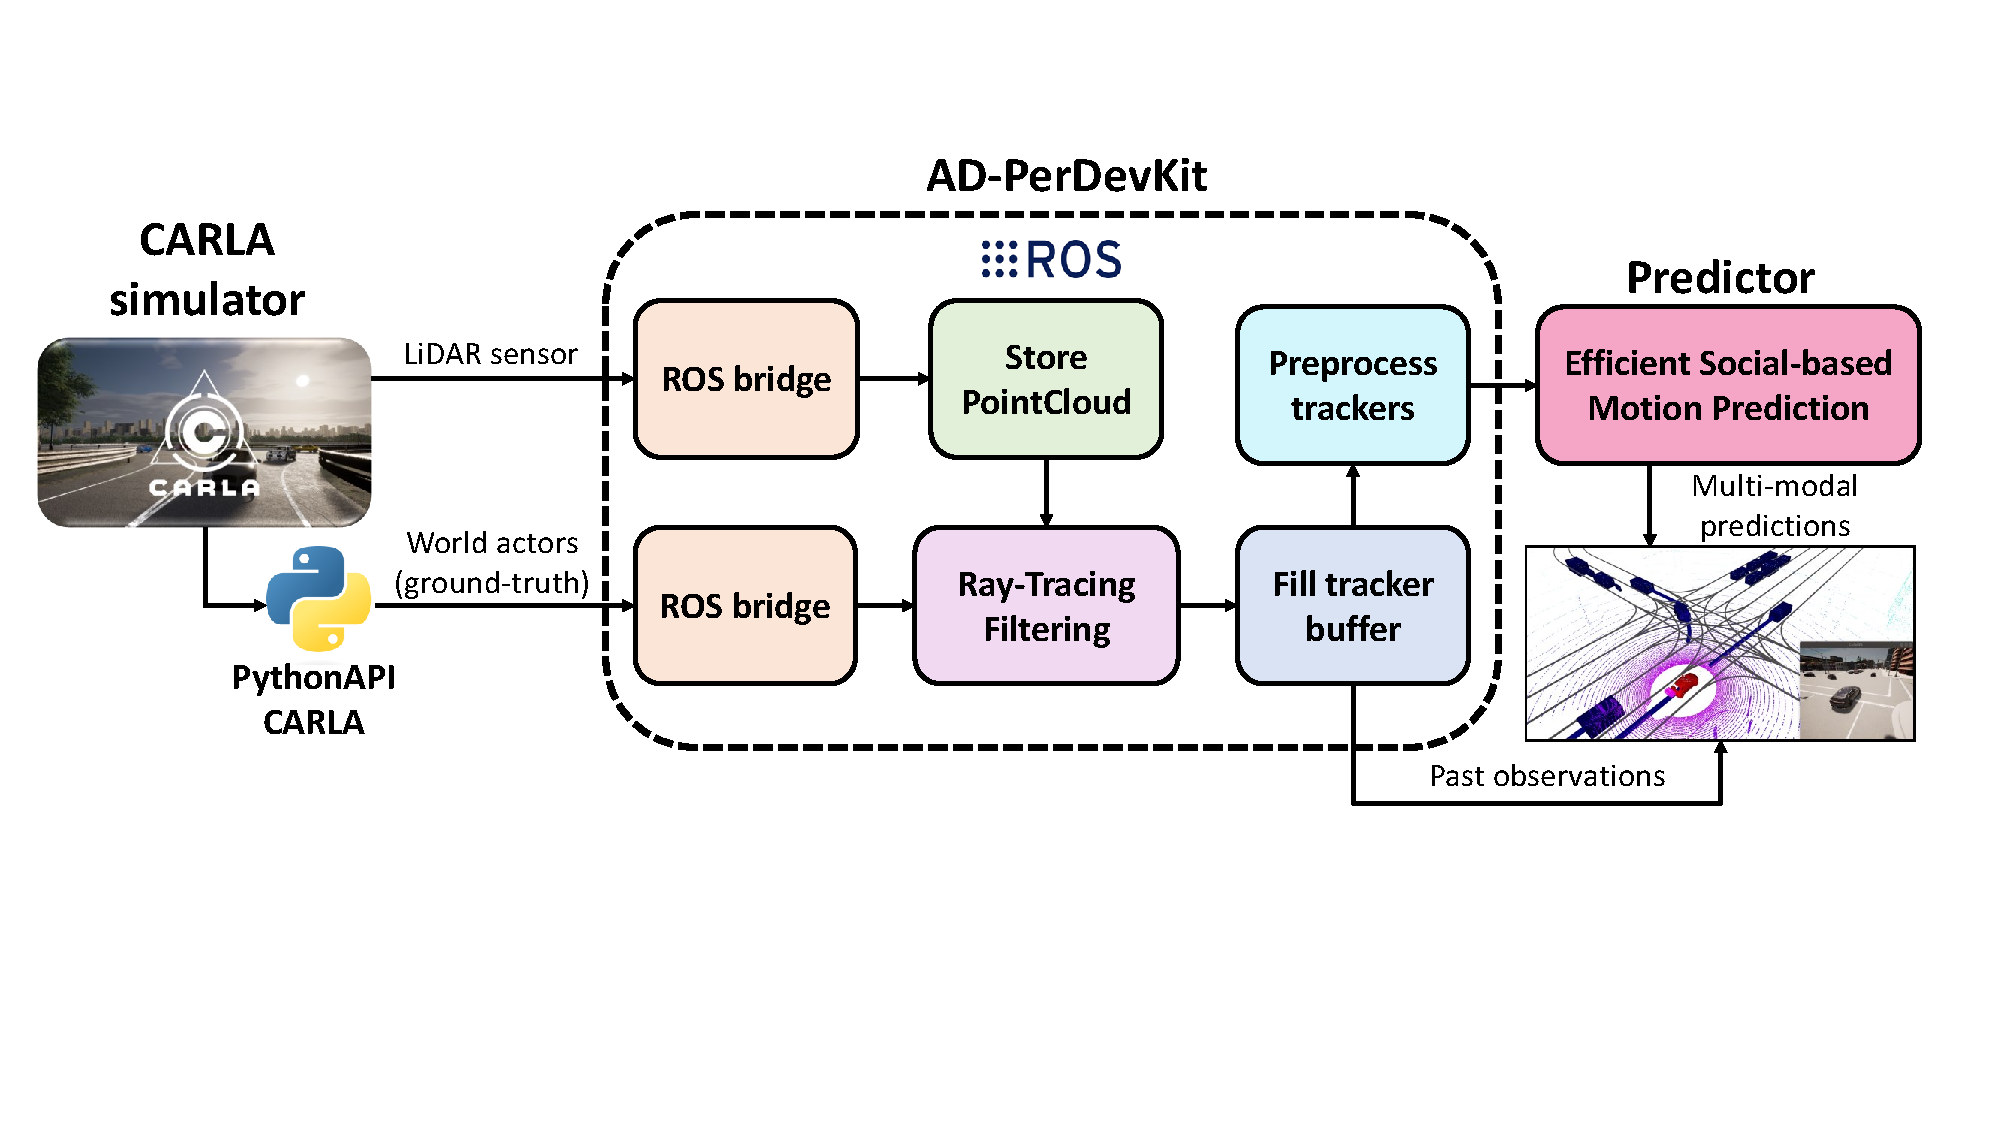
\includegraphics[width=\textwidth, trim={0 4cm 0 1cm},clip]{chapter_8_Applications/ad_perdevkit.pdf}
	\captionsetup{justification=justified}
	\caption[Overview of the integration of our prediction pipeline in the \ac{CARLA} simulator using the AD-PerDevKit tool]{Overview of the integration of our prediction pipeline in the \ac{CARLA} simulator using the AD-PerDevKit tool. The PythonAPI module is used to obtain all actors in the world. Our \ac{AD-PerDevKit} performs a ray-tracing-based filtering to keep only those obstacles which are hit by at least one \ac{LiDAR} ray. Past observations are considered over time for these relevant obstacles which are used to feed the social-based prediction pipeline.}
	\label{fig:chapter_8_Applications/ad_perdevkit}
\end{figure}

\subsection{Autonomous Driving Perception Development Kit (AD-PerDevKit)}
\label{subsec:8_ad_perdevkit}

As stated above, most \ac{SOTA} \ac{MP} pipelines in the field of \ac{AD} require 360\degree \ac{DAMOT} to get the past observations of the agents and then predict their future actions. Since this thesis is not focused neither in object detection nor tracking, which would involve significant complexity and effort, surpassing the intended focus of this research, utilizing ray-tracing-based ground-truth as a realistic representation of the environment is a justifiable decision.

Autonomous driving systems rely on accurate and reliable input data to make informed decisions. Ray-tracing techniques, which simulate the behavior of light in a virtual environment, provide a highly realistic representation of the surroundings. By employing ray-tracing-based ground-truth, precise information about the positions, shapes, and properties of obstacles in the environment can be generated as preliminary information before conducting the prediction stage. This approach ensures that the \ac{ADS} receives high-fidelity data that closely resembles real-world conditions. 

Moreover, the offline nature of the ground-truth generation process allows for flexibility in experimentation, debugging, and analysis, which can significantly benefit the development and evaluation of the prediction algorithm. For example, by storing the ground-truth of a whole scenario as a text file, do the same with the output predictions, and finally obtain the same metrics that the original dataset where the model was trained to check the domain adaptation (that is, if the model works fine or not without fine-tuning with the current environment data).

The main contribution of the AD-PerDevKit is the creation of a ground-truth generation tool for the surrounding obstacles of the ego-vehicle using CARLA and ROS. For its implementation, the CARLA-ROS brige is used so that the simultaneous execution of CARLA and this tool is not necessary, since the execution of both programs can be very demanding due to the simulator requirements. This way it is possible to record a rosbag (a file with all the ROS messages) with the GT information, so that only an area around the ego-vehicle is analyzed and not the whole obstacles in the CARLA runtime.

The messages created by CARLA contain the information of the different objects of the environment in relation to the map on which it is being used. However, to be used independently, the obstacles must be referenced to the ego-vehicle. Therefore, it is necessary to perform the different transformations to go from a coordinate system based on the map to a coordinate system based on the ego-vehicle.

\subsubsection{Ray-Tracing-based Filtering}
\label{subsubsec:8_ad_perdevkit_object_visibility}

One main issue for the \ac{GT} calculation is that \ac{CARLA} always render all the objects, even when they are not visible by the camera, LiDAR or Radar, which is a problem for any training or validation process. In other words, it is necessary to calculate the visibility of the objects from the vehicle, since, otherwise, when proceeding with the evaluation, the precision of the models would be reduced due to not being able to detect some occluded or invisible objects. As aforementioned, to solve that calculation of object visibility (\ie \ an object that could be preliminarily observed by a \ac{SOTA} sensor fusion module), we make use of the ray-tracing paradigm.

There are many studies about ray tracing that solve this issue. These techniques \cite{raytracing1, raytracing2} are computationally very expensive so it is very difficult to implement them in real-time. In that sense, we propose a method using directly the point-cloud calculated by the simulator. Regarding this, a vehicle will be considered as visible, as long as a point of the LiDAR point-cloud is found inside an object, in the same way as it is done in the nuScenes dataset \cite{caesar2020nuscenes}. 

Moreover, it is important to note that this tool is designed to work either for offline or online \ac{GT} generation. On the other hand, one of the most important and delicate parts for the real-time use of this application is efficiency, so it is necessary to perform a method similar to the \ac{SOTA} in terms of ray-tracing, but with low computational cost. Therefore, it was decided to use the latest point-cloud processed by our custom \ac{ROS} bridge to filter the objects in the environment given a frequency of 10 Hz (standard in the \ac{AD} industry, and particularly in the \ac{CARLA} Autonomous Driving Leaderboard). For the implementation of this operation, vectorization of the operations is necessary, as computation needs to be done in less than $10^{-2}$ seconds. It must be noted that only vehicles and pedestrians are considered for our purposes, since \ac{CARLA} also provides the traffic lights and other traffic infrastructure as World agents or actors. The steps to be performed are the summarized in Algorithm \ref{alg:8_ray_tracing_object_visibility}, where a maximum distance of 120 m is considered to filter the furthest agents:

\begin{algorithm}[H]
	\SetAlgoLined
	\footnotesize
	\SetKwInOut{Input}{Input}
	\SetKwInOut{Output}{Output}
	
	\Input{\ac{LiDAR} raw data and \ac{CARLA} World objects}
	\Output{Bounding box parameters of visible agents}
	
	\BlankLine
	
	Transform \ac{LiDAR} raw data and \ac{CARLA} World objects into \ac{ROS} format to enhance matrix operations and interpretability.
	
	\BlankLine
	
	Remove objects further than the maximum \ac{LiDAR} distance.
	
	\BlankLine
	
	Delete points in the point cloud with heights higher or lower than the objects in the surroundings.
	
	\textbf{Function} $f_{\text{visible\_bb}}(\text{bb}, \text{points})$:
	
	\Indp
	\Return $\text{np.logical\_and}($
	
	\hspace{3em} $\text{np.logical\_and}(\text{bb}[0] - \frac{\text{bb}[3]}{2} \leq \text{np.array(points}[:,0]),$
	
	\hspace{3em} $\text{np.array(points}[:,0]) \leq \text{bb}[0] + \frac{\text{bb}[3]}{2},$
	
	\hspace{3em} $\text{bb}[1] - \frac{\text{bb}[4]}{2} \leq \text{np.array(points}[:,1])), $
	
	\hspace{3em} $\text{np.logical\_and}(\text{np.array(points}[:,1]) \leq \text{bb}[1] + \frac{\text{bb}[4]}{2},$
	
	\hspace{3em} $\text{bb}[2] - \frac{\text{bb}[5]}{2} \leq \text{np.array(points}[:,2]),$
	
	\hspace{3em} $\text{np.array(points}[:,2]) \leq \text{bb}[2] + \frac{\text{bb}[5]}{2}))$
	
	\Indm
	
	\BlankLine
	
	Select visible objects having at least one point in the pointcloud, considering the rotation of different objects.
	
	\BlankLine
	
	\textbf{If} pointcloud data is available:
	
	\Indp
	$points\_in\_bb \gets f_{\text{visible\_bb}}((\text{obj.position\_x}, \text{obj.position\_y},$
	
	\hspace{9.5em} $\text{obj.position\_z, obj.l, obj.w, obj.h}), \text{self.pointcloud})$
	
	$n\_points\_in\_bb \gets \text{np.add.reduce}(points\_in\_bb)$
	
	\Indm
	
	\BlankLine
	
	\caption{Ray-tracing-based filtering algorithm to perform object visibility in the \ac{AD-PerDevKit}}
	\label{alg:8_ray_tracing_object_visibility}
\end{algorithm}

\subsection{Experimental results}
\label{subsec:8_experimental_results}

Once we have calculated the 360\degree~visible objects in a frame $t$, as additional preprocessing steps the \ac{AD-PerDevKit} tool fills a buffer with the past positions of the corresponding agent (simulating a real-world buffered Multi-Object Tracker). Note that if the buffer of an agent was created and in a given frame $t$ it is occluded, the observation at that particular timestamp (in the same way than computed in previous Chapters) is filled with zeros and the binary flag $b_i^t$ set to 1, indicating that the observation $t$ of the agent $i$ has been padded. 

Nevertheless, since the proposed prediction model has been trained in Argoverse 2 using an observation length of \textit{$obs_{len}$} = 50 (\ie \ 5s of motion history regarding a frequency of 10 Hz). Then, calculating the predictions with only 2 or 3 observations would not make sense, since even though there are several agents in Argoverse 1 and Argoverse 2 with only few observations (for example, an object is relevant in the scene since it is relevant to the \ac{ADS} in $t=0$, with only has 4 observations because suddenly appeared in the traffic scenario), most agents should not be predicted with such a low number of observations. To this end, we filter those obstacles with a number of observations less than a certain threshold, set to 30 in this case. Figure \ref{fig:chapter_8_Applications/use_cases/simulator_CARLA_RVIZ} depicts an example in Town03 of the \ac{AD-PerDevKit} output while driving our \ac{ADS} in the \ac{CARLA} simulator. We illustrate the past observations (until \textit{$obs_{len}$} = 50) of the relevant agents such as \textbf{\textcolor{blue}{vehicles}} (cars, vans, trucks, buses) and \textbf{\textcolor{brown}{VRUs}} (cyclists, motorcyclists and pedestrians), as well as the \textbf{\textcolor{red}{ego-vehicle}} observations. All agents have their corresponding identifier.

In terms of prediction, model will be able to predict only if the ego-vehicle has at least two observations, since to compute the rotation angle, at least the current and past observations are required. Moreover, \textbf{\textcolor{ForestGreen}{multi-modal predictions}} are calculated for each agent (including the ego-vehicle, treated as a standard agent, not taking into account the \ac{CMP} paradigm as explained in Chapter \ref{cha:related_works}). Note that for visualization purposes, we avoid plotting the ego-vehicle predictions, other agents modes with a confidence value lower than a certain threshold, in this case set to 0.2. The remaining predictions will be sorted in terms of opacity based on their confidence: the higher the transparency, the less probable the future mode or behavior will be, as illustrated throughout the thesis. Furthermore, even though in \ac{CARLA} our ego-vehicle is a gray Lincoln MKZ 2017, in the \ac{RVIZ} tool, for visualization purposes, it is represented as the red vehicle. Note that, in all traffic scenarios, the model should be able to differentiate between static and dynamic objects, \ie \ the model must reason which agents should keep their position in future frames (\eg \ agents stopped in front of a red traffic light or stop) and which agents, even though they are currently stopped, must be predicted since ahead vehicles have started moving. Dynamic agents, as expected, are predicted in all different situations. 

\begin{figure}[!h]
	\centering
	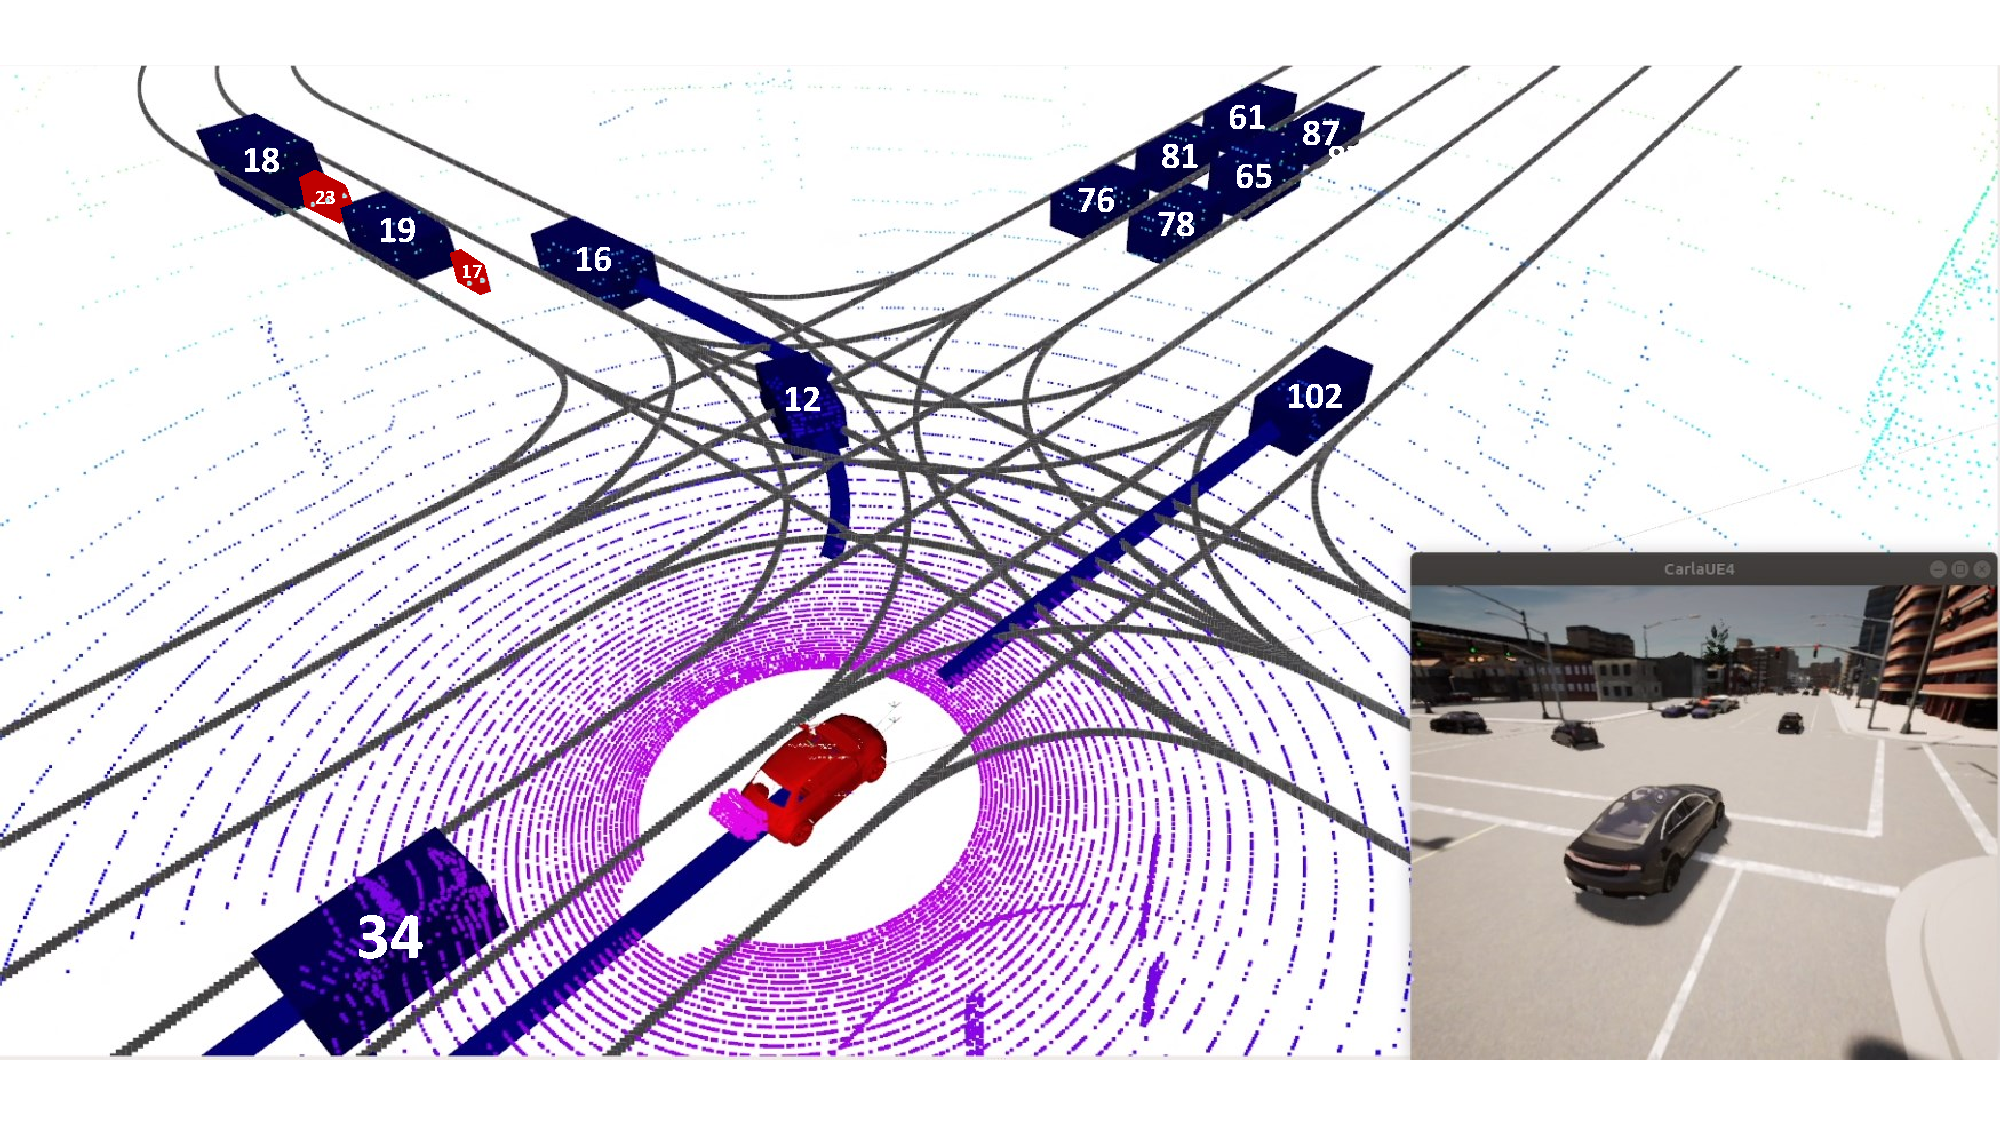
\includegraphics[width=\textwidth]{chapter_8_Applications/scenarios/simulator_CARLA_RVIZ.pdf}
	\captionsetup{justification=justified}
	\caption[Ray-tracing-based filtering and buffered \ac{MOT} example in the \ac{RVIZ} simulator]{Ray-tracing-based filtering example and buffered \ac{MOT} in the \ac{RVIZ} simulator. Past observations (until \textit{$obs_{len}$} = 50) of the relevant agents such as \textbf{\textcolor{blue}{vehicles}} (cars, vans, trucks, buses) and \textbf{\textcolor{brown}{VRUs}} (cyclists, motorcyclists and pedestrians), as well as the \textbf{\textcolor{red}{ego-vehicle}} observations. All agents have their corresponding identifier.}
	\label{fig:chapter_8_Applications/use_cases/simulator_CARLA_RVIZ}
\end{figure}

Experiments were run in a PC desktop computer consisting of an AMD Ryzen 9 5900X 12-Core Processor (overclocked to 3.7 GHz), NVIDIA 3090 RTX Ti and 32 GB of RAM (3200 MHz). To qualitatively validate our prediction pipeline, we have designed several interesting use cases in the \ac{CARLA} simulator using the OpenScenario tool, inspired in the \ac{NHTSA} where a prediction algorithm is of vital importance to take the optimal action in the short/long term, being essential to improve the safety and comfort of both the ego-vehicle and the surrounding environment. As aforementioned, map information is not included in the model for simplicity due to the noticeable amount of work to adapt the \ac{HDmap} format and heuristic lane proposals extraction (as proposed in Chapter \ref{cha:improving_multi_agent}) to a completely different environment. Furthermore, as trained in Argoverse 1 and 2, observations are received at a frequency of 10 Hz from the simulator.

Table \ref{table:8_carla_use_cases} summarizes the proposed use cases, including the following features: Scenario ID, \ac{CARLA} simulator town where it was conducted, use case highlights, total number of actors in the world, ego-vehicle speed, and \ac{minADE} $K$=6, which is the most representative \ac{MP} metric throughout this thesis, and a threshold of minimum of number of observations to start predicting an agent. Note that the number of actors in the \ac{CARLA} is the recommended traffic density for the corresponding town in the \ac{CARLA} Autonomous Driving Leaderboard to avoid unnecessary blockouts specially in crowded roads and intersections.

In order to evaluate the model in the different scenarios, we store the buffers of all observed objects at frame $t$ in a $csv$ file. Then, after the traffic scenario has finished, we have $obs_{len}=50$ observations at frame $t$ per agent, which is the input required by the prediction network in Argoverse 2. Furthermore, it is important to take into account that the \ac{GT} for each timestamp $t$ must be a set of $pred_{len}=60$ 2D \ac{BEV} positions in global coordinates. To this end, as a preprocessing step, given a timestamp (so, its corresponding $csv$ file), we gather the future positions of the agents observed in the current file. If an agent has not been observed at a particular frame in the prediction horizon (\ie \ the agent was not observed in the $39-th$ future step out of 60), that position of the \ac{GT} is masked in such a way it will not be compared with the output of our model. Finally, after having the \ac{GT} of the whole scenario and predictions per frame, we follow standard practices to compute the \ac{minADE} and \ac{minFDE} metrics (both in the uni-modal and multi-modal scenario). As observed in Figures \ref{fig:chapter_8_Applications/scenarios/scenario_1/scenario_1_quantitative}, \ref{fig:chapter_8_Applications/scenarios/scenario_2/scenario_2_quantitative}, \ref{fig:chapter_8_Applications/scenarios/scenario_3/scenario_3_quantitative} and \ref{fig:chapter_8_Applications/scenarios/scenario_4/scenario_4_quantitative}, at the end of the scenarios the metrics are closed to zero since the number of future steps start decreasing from $frames_{total}-60$, in such a way we can only compare our predictions with the nearest future steps (from long-term to short-term, because other positions of the \ac{GT} are masked). Further details and code to generate the \ac{GT} and calculate the metrics may be found in the final \href{https://github.com/Cram3r95/argo2goalmp}{open-source} \footnote{https://github.com/Cram3r95/argo2goalmp} proposal of this thesis. 

\begin{table}[]
	\centering
	\captionsetup{justification=justified}
	\caption{Summary of use cases conducted in the \ac{CARLA} to study the domain adaptation of our efficient social-based \ac{MP} algorithm}
	\label{table:8_carla_use_cases}
	\resizebox{\linewidth}{!}{
		\begin{tabular}{c|c|c|c|c|c|c}
			\toprule
			Scenario ID & Town & Use case & Actors & Ego max-vel & \ac{minADE} ($K$=6) $\downarrow$ & Threshold \\
			 & & highlights & in the world & [km/h] & & min observations \\
			\midrule
			1 & 03 & Stop + 4-ways intersection & 120 & 25.2 & 1.96 & 30 \\
			2 & 04 & Crowded highway & 180 & 54 & 2.52 & 30 \\
			3 & 01 & Red Traffic Light + Unexpected \ac{VRU} & 100 & 25.2 & 1.78 & 3 \\
			4 & 03 & Crowded roundabout & 160 & 36 & 2.81 & 30 \\
			\bottomrule
		\end{tabular}
	}
\end{table} 

% One of the things we realized was the significant influence of the data acquisition frequency to feed the prediction network. As mentioned throughout the thesis, Argoverse 1 and Argoverse 2 provide observations at a rate of 10 Hz (for example, 5 seconds correspond to 50 frames). However, since the prediction network in CARLA has been integrated with the other layers of our reactive autonomous navigation architecture (to avoid running red lights or colliding with an agent), to obtain new data from the simulator (i.e., tick), the system must wait for the most restrictive layer (as expected, the prediction layer) to trigger an output flank to indicate that the current data has been processed. In this regard, it has been observed that the output frequency of the ROS topic from the perception layer, which indicates the end of a simulation cycle, is approximately 8.7 Hz, lower than the 10 Hz specified by Argoverse 1 and 2. Refactoring the perception layer to acquire new simulator data at the same frequency as a network trained in Argoverse 2 is beyond the scope of this thesis.

\subsubsection{Scenario 1: Stop and 4-ways intersection in Town03}
\label{subsubsec:8_experimental_results_scenario_1}

Figures \ref{fig:chapter_8_Applications/scenarios/scenario_1/scenario_1_route22_town03_training}, \ref{fig:chapter_8_Applications/scenarios/scenario_1/scenario_1_quantitative} and \ref{fig:chapter_8_Applications/scenarios/scenario_1_frames_of_interest} show the ego-vehicle conducting a stop maneuver and 4-ways intersection in Town03. The number of agents in the world is set to 120, the maximum velocity for the ego-vehicle is 25.4 km/h, and the minimum number of observations is set to 30. As observed in Figure \ref{fig:chapter_8_Applications/scenarios/scenario_1/scenario_1_quantitative}, the mean value of the \ac{minADE} $K$=6 metric is 1.96, which is noticeable higher than the results obtained in Argoverse 2 with our proposed model without map information (multi-modal $K$=6 \ac{minADE} = 1.19). However, it may be appreciated that most values are up-to-pair with the validated model (1.19) since the average value is greatly increased due to the large error from frames $\simeq$ 700 to $\simeq$ 800 when agents start moving after the corresponding traffic lights change from red to green, and the uncertainty in the prediction stage becomes noticeable higher.

Regarding the stop maneuver (Figures \ref{subfig:chapter_8_Applications/scenarios/scenario_1/scenario_1_stop_carla} and \ref{subfig:chapter_8_Applications/scenarios/scenario_1/scenario_1_stop_rviz} at frame $t$), according to the traffic rules, the ego-vehicle must stop regardless if there are opponents around, so prediction is not required for the first stop. Nevertheless, predicting future behavior is absolutely necessary after making the first stop in order to safely merge into the new lane. It can be observed how the model proposes curved trajectories from straight past trajectories, as well as multi-modality, fundamentally in terms of different velocity profiles. This is because the model understands, based on the deep social features of the scene, that there are not several clearly distinct directions as is the case with an intersection. On the other hand, in the case of the 4-ways intersection, it can be clearly seen how the model is capable of understanding the difference between static objects (waiting behind a red traffic light, so predictions are calculated in the same site than observations), and dynamic objects. For example, agent number 392 (green Chevrolet Impala in Figures \ref{subfig:chapter_8_Applications/scenarios/scenario_1/scenario_1_intersection_carla_t}, \ref{subfig:chapter_8_Applications/scenarios/scenario_1/scenario_1_intersection_rviz_t} at frame $t+240$) presents multi-modality in terms of different possible directions (turn left or go straight) since the model understands that the agent is in an intersection given the surrounding agents and past observations, even though map information is not included. On the other hand, 2 seconds (20 frames) in the future the model reasons that agent 392 has left the intersection and makes multi-modal predictions with different speed profiles in a single direction.

% Figure \ref{fig:chapter_8_Applications/use_cases/stop} illustrates a standard Stop traffic scenario, where the model is clearly able to distinguish among dynamic and static objects, predicting the trajectories in the same point for agents stopped for a while. Moreover, it can be slightly appreciated a multi-modal prediction for the white and red van, but probably the model discards the possibility of turning right given the vehicle that is present in that lane in the current timestamp. Conducting transfer learning and fine-tuning the model with \ac{CARLA} scenarios could be an option to help the models understand the situation in an enhanced way.  

\subsubsection{Scenario 2: Crowded highway in Town04}
\label{subsubsec:8_experimental_results_scenario_2}

Figures \ref{fig:chapter_8_Applications/scenarios/scenario_2/scenario_2_route15_town04_testing}, \ref{fig:chapter_8_Applications/scenarios/scenario_2/scenario_2_quantitative} and \ref{fig:chapter_8_Applications/scenarios/scenario_2_frames_of_interest} illustrate a crowded highway scenario in Town04. The number of agents in the world is set to 180, the maximum velocity for the ego-vehicle is 54 km/h, and the minimum number of observations is set to 30. This situation can be interpreted as a traffic jam, a standard situation when approaching a metropolis in the morning at work time. In this case, we may observe that the model does not compute multi-modal predictions towards different directions, but, as expected, it understands that all vehicles are driving in the same direction (either forward or reverse way) and the multi-modal prediction is computed in terms of different velocity. profiles (that is, the agent can continue with the same velocity, suddenly break or accelerate in the mid/long term).

The mean \ac{minADE} $K$=6 metric throughout the scenario and in general most values throughout the whole scenario are higher than the previous use case (2.52 vs 1.96) whilst from human perspective, a traffic jam should be easier to be predicted than an intersection since most agents present a similar velocity towards the same direction (either forward or reverse way). In that sense, one of the advantages of using our proposed \ac{AD-PerDevKit} pipeline to compute realistic object trackers is that we realize about one of the most important concerns when driving in the \ac{AD} field: object occlusion. Due to the large amount of agents in relatively small areas, \ac{LiDAR} rays are not able to hit the corresponding agents, specially those which are further away from the ego-vehicle. Then, a lot of padding data is introduced to the network at the same time, so the model is not able to properly reason what is happening around. To this end, a possible solution could be integrating the object tracking and motion predictor in the same loop in order to use the most plausible predictions from previous timestamps as object observations if the sensor fusion module and tracker in the short-term cannot estimate the current position of the agent. 

% Figure \ref{fig:chapter_8_Applications/use_cases/crowded_highway} illustrates a traffic jam in crowded highway, for example a standard situation when approaching a metropolis in the morning at work time. In this case, we may observe that the model does not compute multi-modal predictions towards different directions, but, as expected, it understands that all vehicles are driving in the same direction (either forward or reverse way) and the multi-modal prediction is computed in terms of different velocity profiles (that is, the agent can continue with the same velocity, suddenly break or accelerate in the mid/long term).

\subsubsection{Scenario 3: Red Traffic Light and Unexpected \ac{VRU} in Town01}
\label{subsubsec:8_experimental_results_scenario_3}

Figures \ref{fig:chapter_8_Applications/scenarios/scenario_3/scenario_3_route1_town01_training}, \ref{fig:chapter_8_Applications/scenarios/scenario_3/scenario_3_quantitative} and \ref{fig:chapter_8_Applications/scenarios/scenario_3_frames_of_interest} illustrate an urban scenario in Town01 where the ego-vehicle is initially stopped in front of a red traffic light, then turn left in a 3-ways intersection and finally must predict the future behaviour of an unexpected \ac{VRU} (in this particular case, a kid suddenly appears running towards the road from behind a CocaCola vending machine). The number of agents in the world is set to 100, the maximum velocity for the ego-vehicle is 25.2 km/h.

Moreover, as discussed throughout this thesis, predicting the behaviour of \acp{VRU}, such as cyclists or pedestrians, is one of the most critical aspect of an \ac{ADS} to be deployed and scaled to real-world applications in urban scenarios. In that sense, unlike other use cases, in this particular case the minimum number of observations is set to 3. The reason is simple: In order to predict the future actions of a challenging unexpected \ac{VRU} who suddenly appears behind an obstacle (\eg \ a wall, van, vending machine, etc.), we need to reduce the minimum number of observations to get predictions on time in order to perform an emergency break (note that in these experiments the predictions do not feed the \ac{DM} module, but our reactive \ac{ADS}, which includes map monitoring, is able to deal with the unexpected situation).

The mean \ac{minADE} $K$=6 metric (1.78) of the whole scenario is worse than the reference in Argoverse 2 (1.19), but the actual metric in most frames is noticeable smaller than the mean. The model struggles from frame $t=400$ to $t=600$ when the ego-vehicle turns left and suddenly faces an unexpected \ac{VRU}. In terms of the 3-ways intersection, Figures \ref{subfig:chapter_8_Applications/scenarios/scenario_3/scenario_3_rtl_carla_t}, \ref{subfig:chapter_8_Applications/scenarios/scenario_3/scenario_3_rtl_rviz_t} and Figures \ref{subfig:chapter_8_Applications/scenarios/scenario_3/scenario_3_rtl_carla_t+20}, \ref{subfig:chapter_8_Applications/scenarios/scenario_3/scenario_3_rtl_rviz_t+20} depict the traffic scenario at frame $t$ and $t+20$ respectively. In that sense, the vehicle 423 is approaching to the intersection. Since the model lacks of map information, it predicts keeping straight and turning right. Then, 2s in the future, due to its past motion (velocity and orientation, which are implicit in the relative displacements), the model correct computes all predictions in the same direction with different velocity profiles.

Finally, at the end of the scenario the ego-vehicle faces the unexpected \ac{VRU} (Figures \ref{subfig:chapter_8_Applications/scenarios/scenario_3/scenario_3_VRU_carla_t}, \ref{subfig:chapter_8_Applications/scenarios/scenario_3/scenario_3_VRU_rviz_t} and Figures \ref{subfig:chapter_8_Applications/scenarios/scenario_3/scenario_3_VRU_carla_t+5}, \ref{subfig:chapter_8_Applications/scenarios/scenario_3/scenario_3_VRU_rviz_t+5} depict the traffic scenario at frame $t+145$ and $t+147$ respectively). Despite the fact that the model only has 3 observations out of $obs_{len}=50$ to start predicting (remaining observations are padded with zeros), preliminary intentions are correctly computed with the corresponding velocity. Moreover, 2 frames later, due to the lack of past information, the model cannot decide a particular behaviour for the kid and still predicts the future actions in completely different directions, which is coherent given the nature of agent.

As observed, even though the model struggles in a particular moment of the traffic scenario, changing the minimum number of observations from 30 to 3 only increases the error at the beginning of the sequence when the model misses past information from the agents. However, in steady state (that is, when most of the agents have the observation buffer filled), the prediction accuracy is similar to the previous use cases.

An interesting point of view for future works could be how to assign the optimal minimum number of observations in the pipeline, or if it can depend on the agent type or potential risks associated to the traffic situation. Better predictions are usually associated to enriched past information (\ie \ more data), so for vehicles it make sense to have at least 30 observations. Nevertheless, for \acp{VRU}, even though the model has been trained with way more past observations, it should predict the agent behaviour as fast as possible in spite of the fact that several modes are computed in non-plausible or non-sense directions.

\subsubsection{Scenario 4: Crowded roundabout in Town03}
\label{subsubsec:8_experimental_results_scenario_4}

Figures \ref{fig:chapter_8_Applications/scenarios/scenario_4/scenario_4_quantitative}, \ref{fig:chapter_8_Applications/scenarios/scenario_4/scenario_4_quantitative} and \ref{fig:chapter_8_Applications/scenarios/scenario_4_frames_of_interest} illustrate one of the most challenging traffic situations in urban scenarios, that is, a roundabout full of agents in Town03, considering incoming, outcoming and present agents in the current time-stamp. The number of agents in the world is set to 160, the maximum velocity for the ego-vehicle is 36 km/h, and the minimum number of observations is set to 30. 

To help the behavioural and local planning modules to take the optimal action, the model clearly predicts the circular motion of the agents, either for the agents that are in the roundabout with different velocity profiles or even for the incoming agents which are going to get into the roundabout and probably intersect with the trajectory of our ego-vehicle if the adversary does not respect the give-way traffic signal.

The mean \ac{minADE} $K$=6 metric (2.81) of the whole scenario is the worst among all proposed scenarios, due to the huge difficulty of predicting the future motion of the agents in a roundabout without map information. There are some agents (such as 405 and 289) which are turning left (roundabout direction is counter-clockwise) and once they leave the roundabout, they are turning right, which is quite difficult to predict without the geometrical constraints, as well as semantic and topological information, of the road. 

Moreover, in a similar way to the Scenario 2 (crowded highway), due to the large amount of agents (either vehicles or \acp{VRU}), as well as the fountain in the middle of the roundabout, there are many occlusions (\eg \ object 376 in Figure \ref{subfig:chapter_8_Applications/scenarios/scenario_4/scenario_4_roundabout_rviz_t}) which generate way more discontinuous past trajectories than in the training dataset, making difficult the generalization of the model. Conducting transfer learning and fine-tuning the model with \ac{CARLA} scenarios could be an option to help the models understand high-complex situation in an enhanced way. 

As observed, understanding this complex situation and taking account all different scenarios, from least dangerous to most optimistic, is the key to build a robust and reliable architecture.

% Finally, Figure \ref{fig:chapter_8_Applications/use_cases/roundabout} shows one of the most challenging traffic situations in urban scenarios, that is, a roundabout full of agents, considering incoming, outcoming and present agents in the current time-stamp. To help the behavioural and local planning modules to take the optimal action, the model clearly predicts the circular motion of the agents, either for the agents that are in the roundabout with different velocity profiles or even for the incoming agents which are going to get into the roundabout and probably intersect with the trajectory of our ego-vehicle if the adversary does not respect the give-way traffic signal. Then, understanding this complex situation and taking account all different scenarios, from least dangerous to most optimistic, is the key to build a robust and reliable architecture.

\section{Summary}
\label{sec:8_summary}

In this Chapter we have evaluated our efficient social-based prediction model, where the incorporation of map information has been avoided for simplicity purposes, since the model has been evaluated in two frameworks, the \ac{SMARTS} and \ac{CARLA} simulators respectively, with a map graph structure way different to Argoverse 2.

In terms of the decision-making application, the prediction module must calculate the future positions of vehicles within the scenario to improve a Reinforcement Learning-based Decision Making module. The results of the study demonstrate that our approach achieves significant performance improvements, particularly in scenarios involving high velocities.

On the other hand, we have successfully integrated the prediction algorithm in our \ac{ADS} in simulation using CARLA and studied the domain adaptation of the algorithm from a static dataset (Argoverse 2) to an hyper-realistic environment, using some scenarios inspired in the well-established \ac{NHTSA} typology. Given the amount of work and complexity required to develop an efficient and accurate 360 \degree \ac{DAMOT} pipeline, we make use of the \ac{AD-PerDevKit} pipeline to generate a realistic \ac{GT} given a ray-tracing-based filtering algorithm and some pre-processing steps to obtain a buffer of past observations for each agent, removing those agents with a number of observations lower than a certain threshold, as a preliminary stage before feeding the prediction module. As observed, the model is able to compute multi-modal predictions in terms of different directions and velocity profiles, or even predicting the trajectories in the same point for agents stopped for a while, understanding the past motion and complex interactions among the agents and corresponding neighbours. 

% This research opens up several potential directions for future work. The proposed approach can be evaluated in a broader range of urban driving scenarios to assess its robustness and scalability, up-to-pair with the difficulty of the Argoverse 2 dataset scenarios (specially in terms of intersections or lane change behaviours at high speed) where multimodal predictions with higher prediction horizons will be required. Furthermore, the Reinforcement Learning-based Decision Making module can be enhanced by exploring advanced algorithms.

\begin{comment}
	IDEAS:
	
	1. Con el ADS que hay estable, dejarlo otra vez pulido y optimizado en poco tiempo (creo que YOLO está duplicada, PointPillars no corría bien, etc., y eso se puede poner como GT en el R-VIZ, diciendo específicamente que es GT). 
	
	Eso, con el AD-PerDevKit, estimo que fuesen dos días de trabajo.
	
	2. Ya se hicieron pruebas para meter el by-pass de tracking (hecho en SMARTS/SUMO) en CARLA, y funciona bien, aunque hay que retocar.
	
	3. Mi idea es correr el ADS en las rutas del Leaderboard, y obtener scores, sin nada más que lo estable ahora mismo vs meter predicción + dm con RL sobre todo en intersecciones (las decisiones de la red de rodrigo fuera de intersecciones están capadas)
	
	4. Hacer comparativas múltiples:
	
	ADS sin predicción
	ADS sin predicción, con DM en intersecciones (sólo basado en posición)
	ADS con predicción y DM en intersecciones (basado en predicción)
	
	Y la teoría dice que cuanta más capacidad predictiva metas al sistema, mejores deberían ser las métricas holísticas.
	
	Si todo fuese bien, y hasta la fecha de la lectura, mi idea es ayudar al equipo a meter detección, fusión y tracking en simulación y real, aunque no sean integraciones mid-level, y quitar el by-pass, pero lo anterior es más prioritario.
\end{comment}

\newpage

% Scenario 1

\begin{figure}[]
	\centering
	\fbox{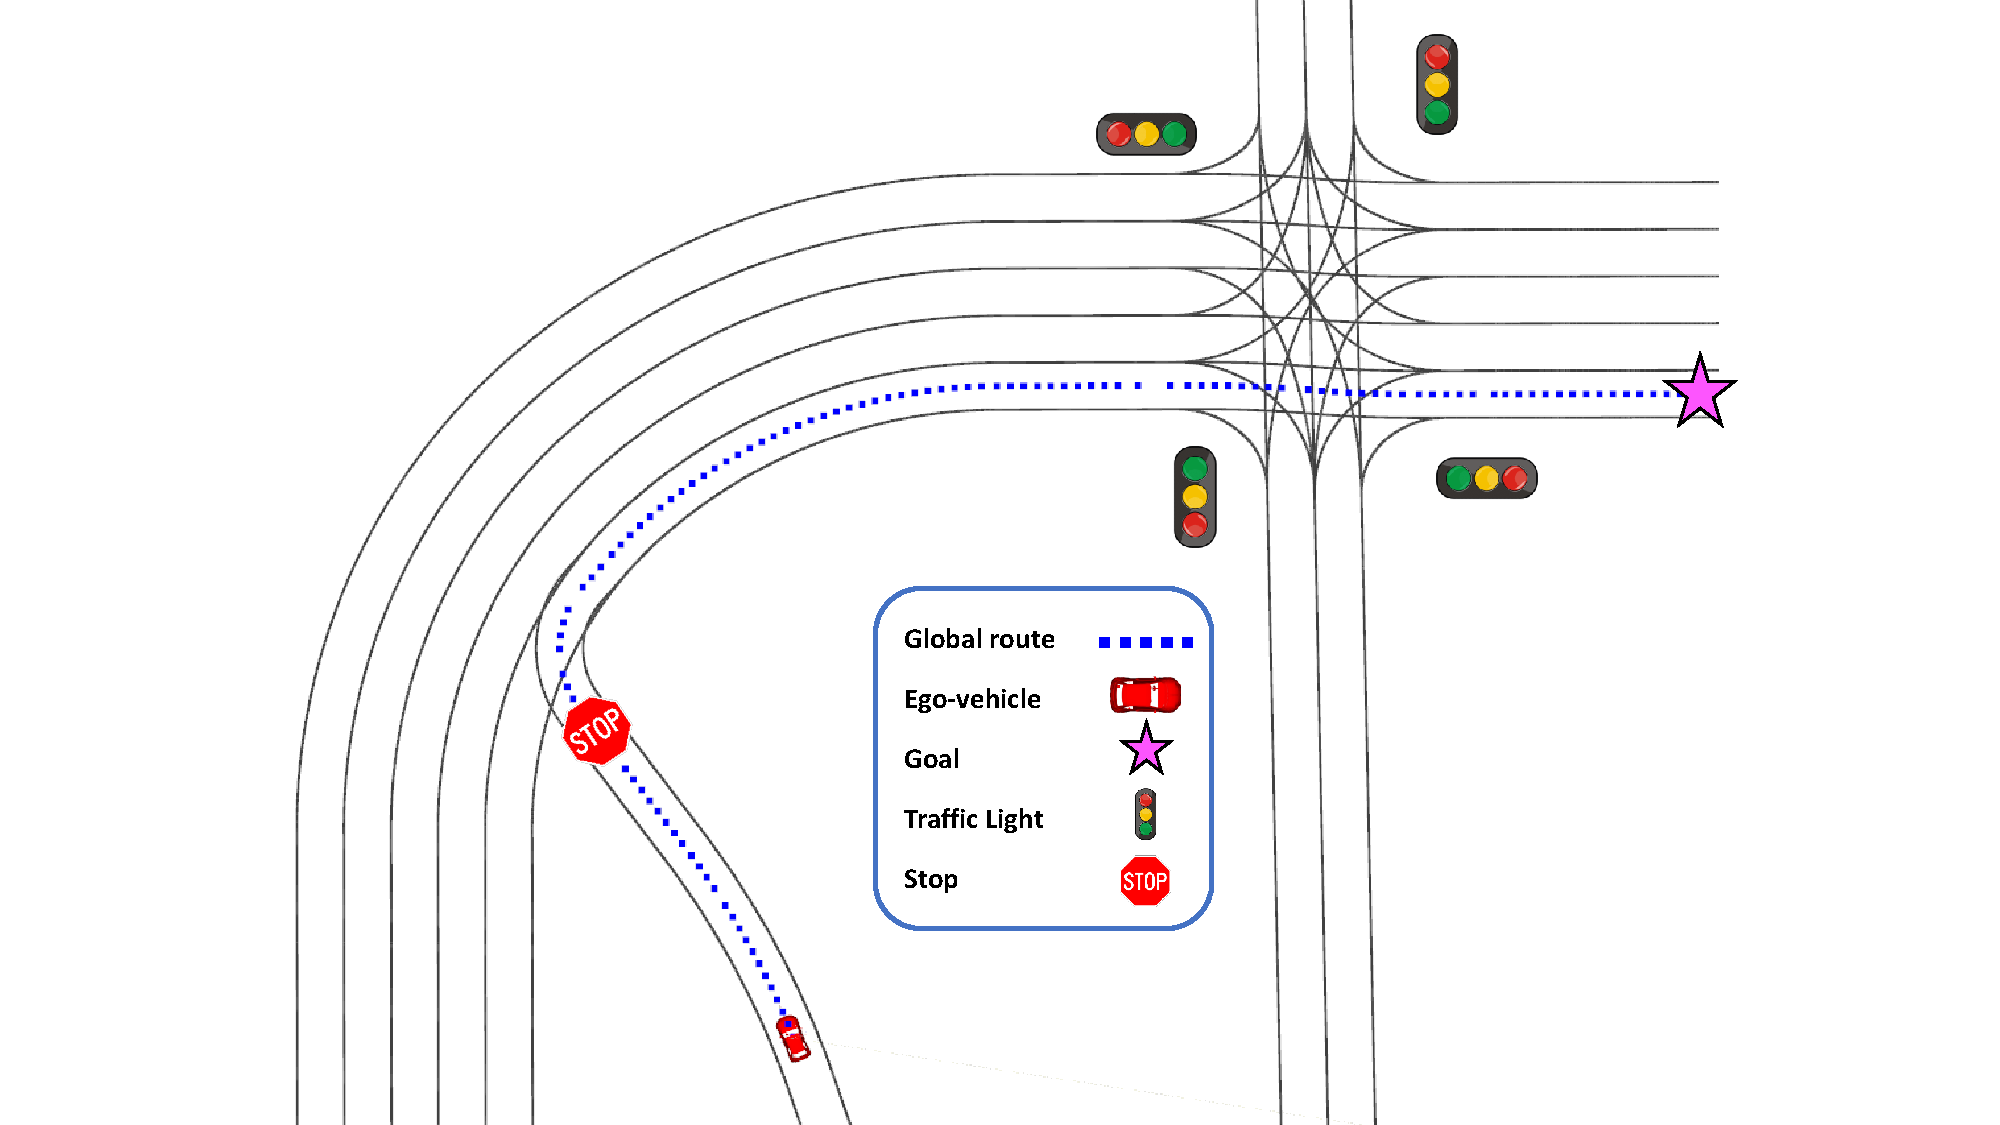
\includegraphics[width=0.8\textwidth, trim={4cm 0 4cm 0},clip]{chapter_8_Applications/scenarios/scenario_1/scenario_1_route22_town03_training.pdf}}
	%\captionsetup{justification=justified}
	\caption{Scenario 1 overview: Stop and 4-ways intersection}
	\label{fig:chapter_8_Applications/scenarios/scenario_1/scenario_1_route22_town03_training}
\end{figure}

\begin{figure}[]
	\centering
	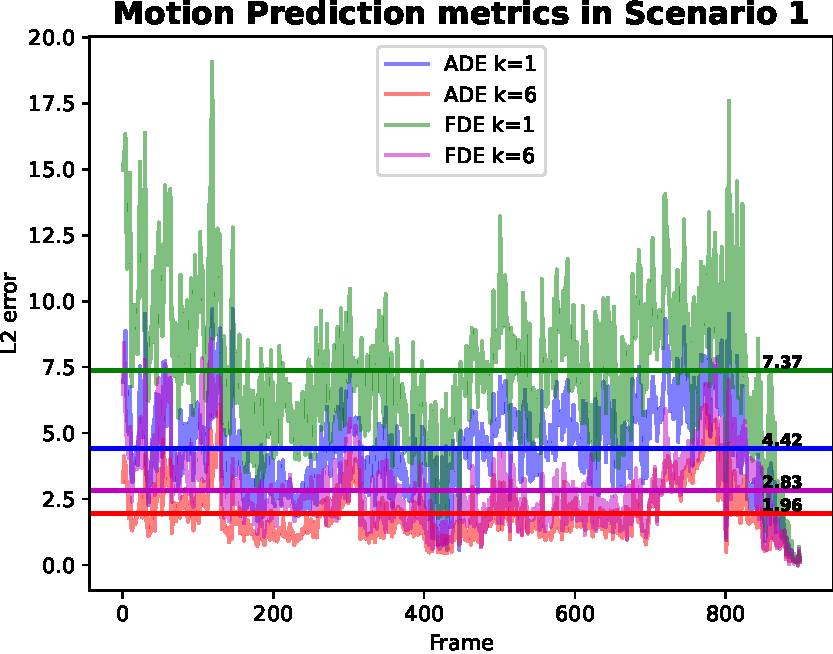
\includegraphics[width=0.9\textwidth]{chapter_8_Applications/scenarios/scenario_1/scenario_1_quantitative.pdf}
	\captionsetup{justification=justified}
	\caption[Scenario 1 quantitative results]{Scenario 1 quantitative results. Constant lines represent the mean value for the corresponding metric throughout the whole scenario.}
	\label{fig:chapter_8_Applications/scenarios/scenario_1/scenario_1_quantitative}
\end{figure}

\begin{figure}[]
	\begin{subfigure}[b]{0.48\textwidth}
		\centering
		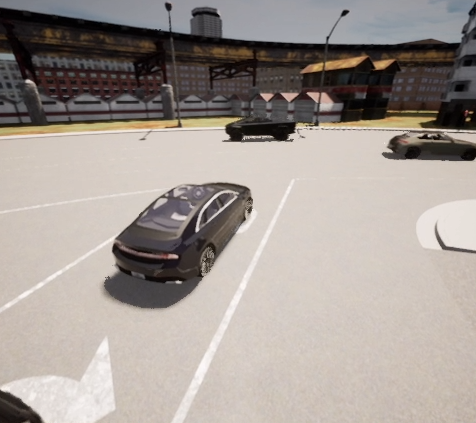
\includegraphics[width=\textwidth]{chapter_8_Applications/scenarios/scenario_1/scenario_1_stop_carla.png}
		\caption{\ac{CARLA} at frame $t$}
		\label{subfig:chapter_8_Applications/scenarios/scenario_1/scenario_1_stop_carla}
	\end{subfigure}
	\hfill
	\begin{subfigure}[b]{0.48\textwidth}
		\centering
		\fbox{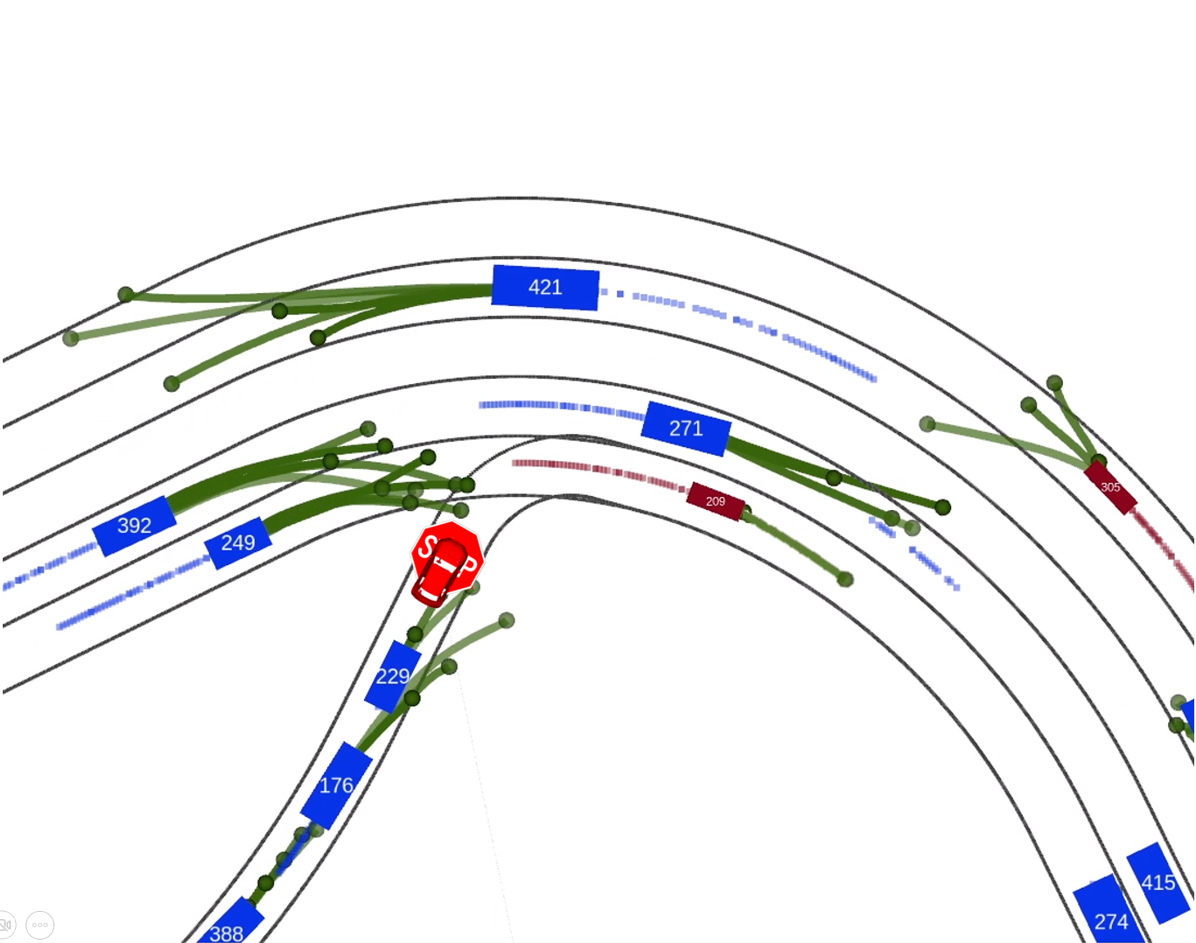
\includegraphics[width=\textwidth, trim={1.8cm 0 1cm 0.2cm},clip]{chapter_8_Applications/scenarios/scenario_1/scenario_1_stop_rviz.png}}
		\caption{\ac{RVIZ} at frame $t$}
		\label{subfig:chapter_8_Applications/scenarios/scenario_1/scenario_1_stop_rviz}
	\end{subfigure}
	\tabularnewline
	\begin{subfigure}[b]{0.48\textwidth}
		\centering
		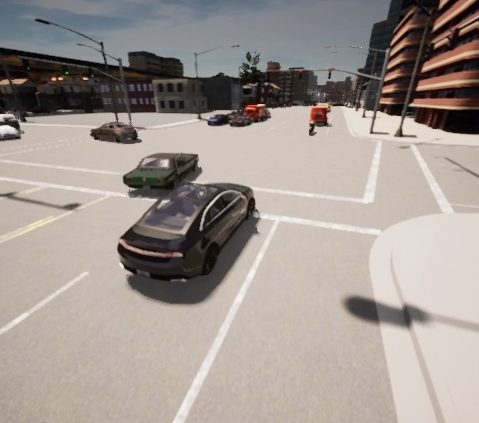
\includegraphics[width=\textwidth]{chapter_8_Applications/scenarios/scenario_1/scenario_1_intersection_carla_t.png}
		\caption{\ac{CARLA} at frame $t+240$}
		\label{subfig:chapter_8_Applications/scenarios/scenario_1/scenario_1_intersection_carla_t}
	\end{subfigure}
	\hfill
	\begin{subfigure}[b]{0.48\textwidth}
		\centering
		\fbox{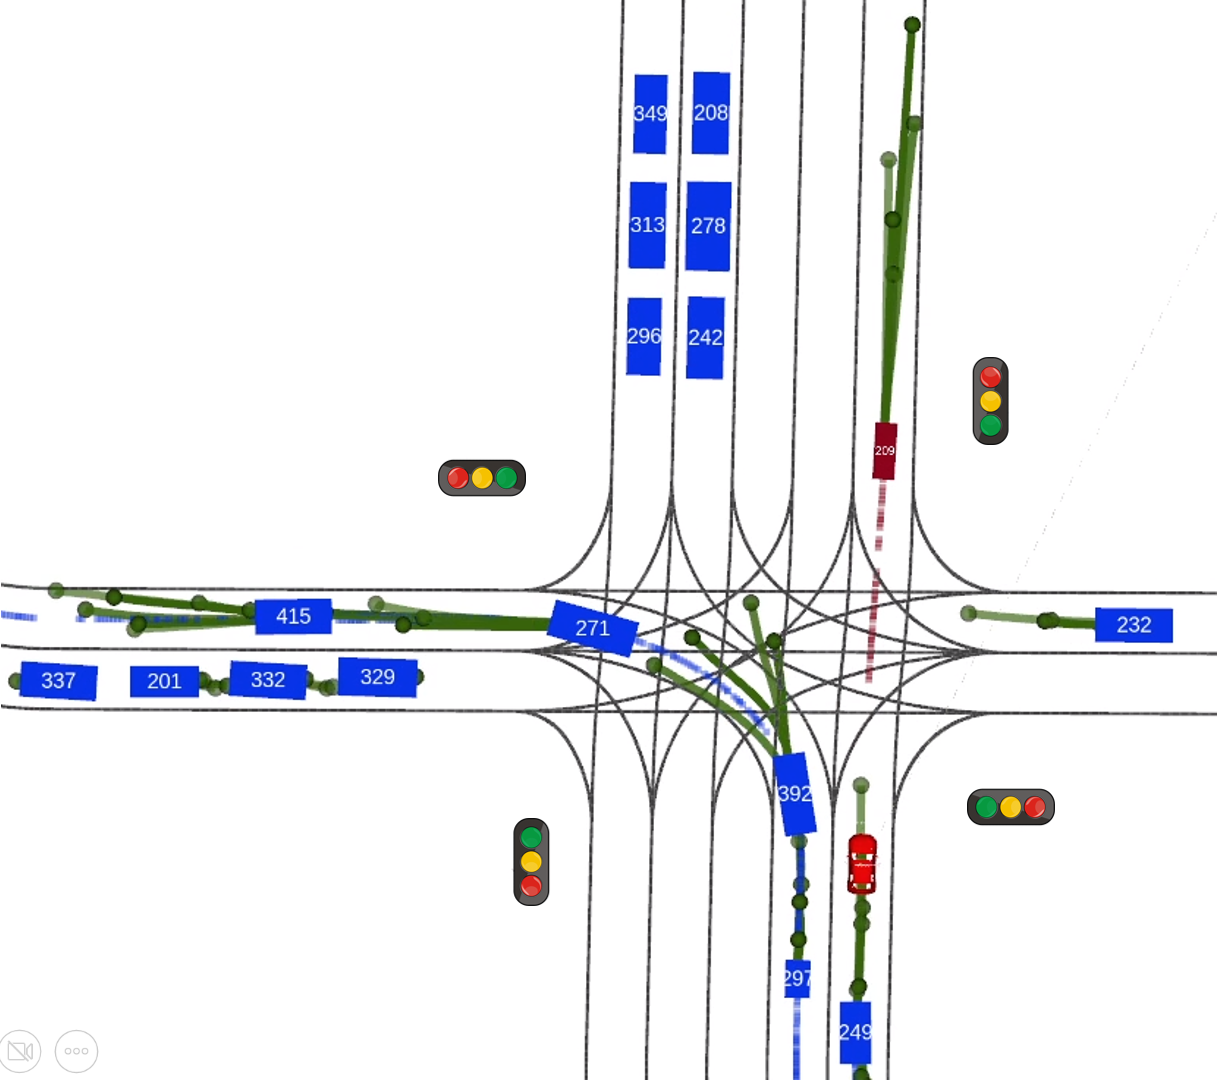
\includegraphics[width=\textwidth, trim={0 0 0 0},clip]{chapter_8_Applications/scenarios/scenario_1/scenario_1_intersection_rviz_t.png}}
		\caption{\ac{RVIZ} at frame $t+240$}
		\label{subfig:chapter_8_Applications/scenarios/scenario_1/scenario_1_intersection_rviz_t}
	\end{subfigure}
	\tabularnewline
	\begin{subfigure}[b]{0.48\textwidth}
		\centering
		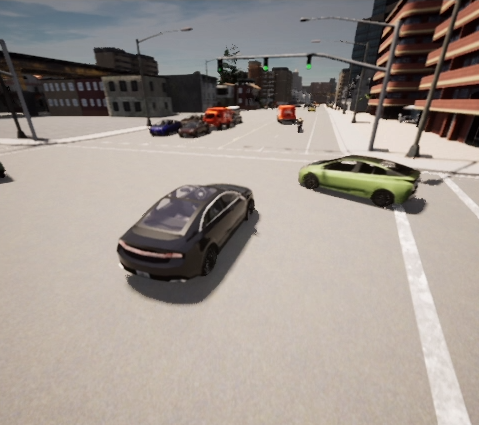
\includegraphics[width=\textwidth]{chapter_8_Applications/scenarios/scenario_1/scenario_1_intersection_carla_t+40.png}
		\caption{\ac{CARLA} at frame $t+260$}
		\label{subfig:chapter_8_Applications/scenarios/scenario_1/scenario_1_intersection_carla_t+40}
	\end{subfigure}
	\hfill
	\begin{subfigure}[b]{0.48\textwidth}
		\centering
		\fbox{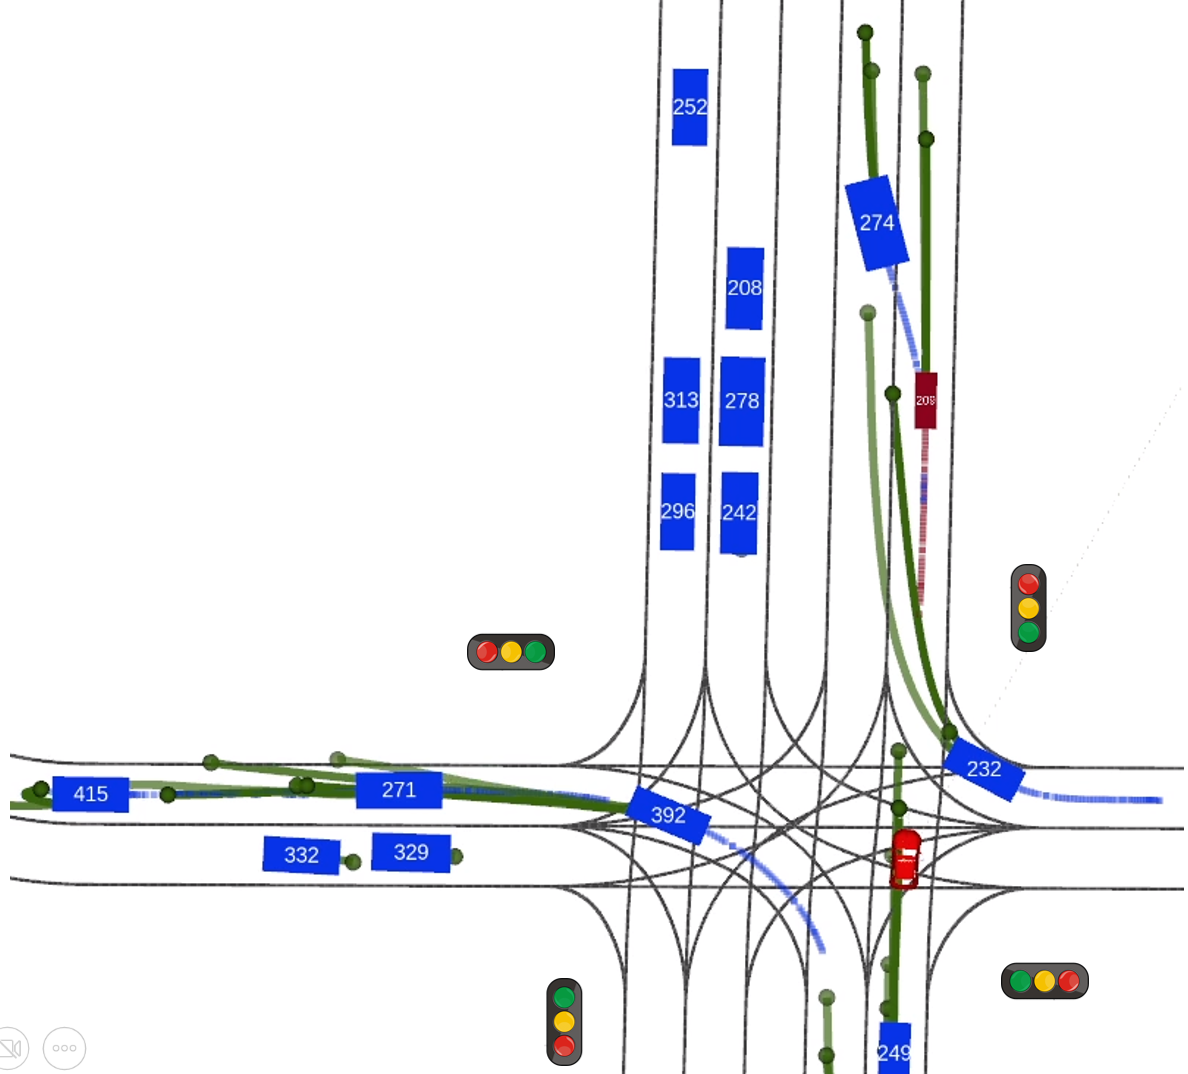
\includegraphics[width=\textwidth, trim={0 0 0 0.5},clip]{chapter_8_Applications/scenarios/scenario_1/scenario_1_intersection_rviz_t+40.png}}
		\caption{\ac{RVIZ} at frame $t+260$}
		\label{subfig:chapter_8_Applications/scenarios/scenario_1/scenario_1_intersection_rviz_t+40}
	\end{subfigure}
	\tabularnewline
	%\captionsetup{justification=justified}
	\caption{Scenario 1 frames of interest}
	\label{fig:chapter_8_Applications/scenarios/scenario_1_frames_of_interest}
\end{figure}

% Scenario 2

\begin{figure}[]
	\centering
	\fbox{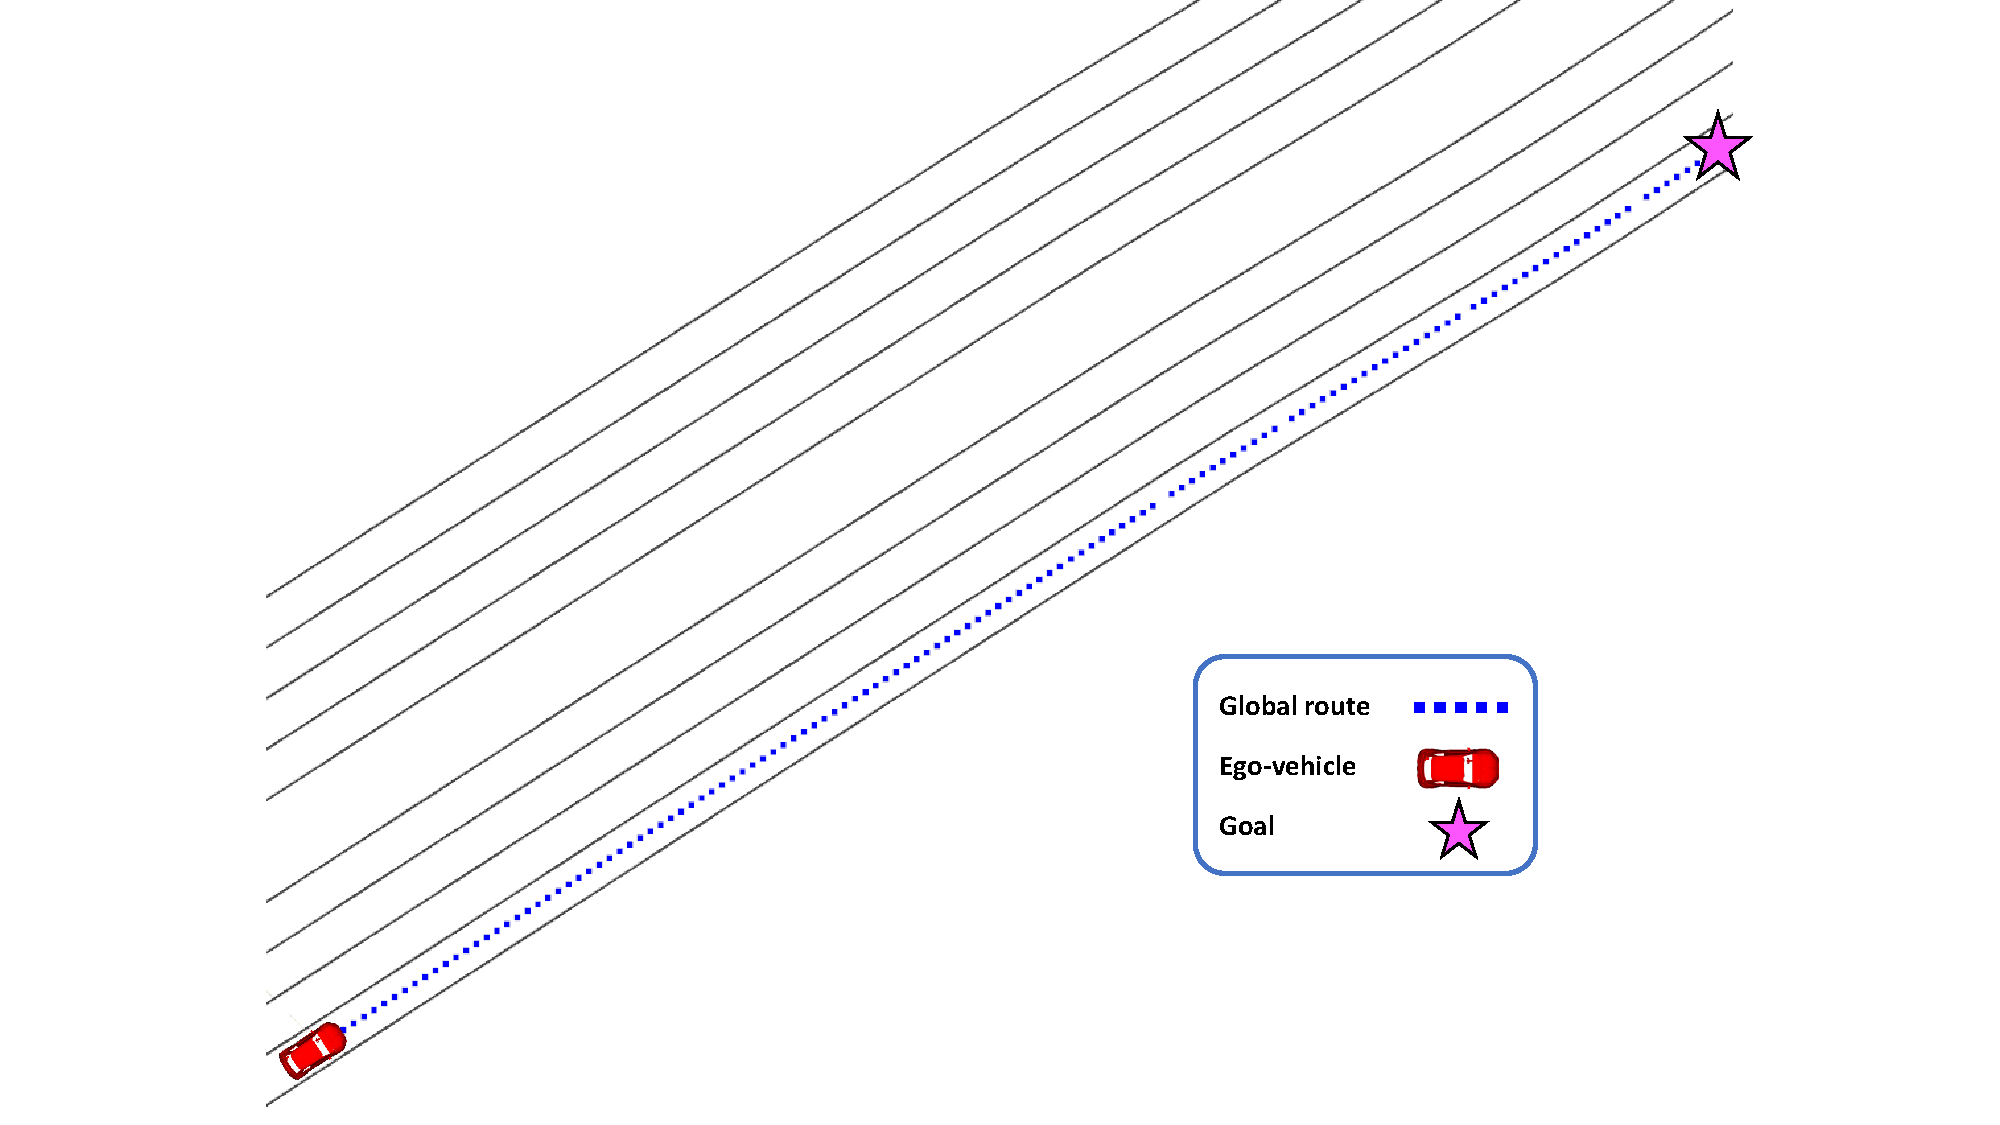
\includegraphics[width=0.9\textwidth, trim={4cm 0 4cm 0},clip]{chapter_8_Applications/scenarios/scenario_2/scenario_2_route15_town04_testing.pdf}}
	%\captionsetup{justification=justified}
	\caption{Scenario 2 overview: Crowded highway}
	\label{fig:chapter_8_Applications/scenarios/scenario_2/scenario_2_route15_town04_testing}
\end{figure}

\begin{figure}[]
	\centering
	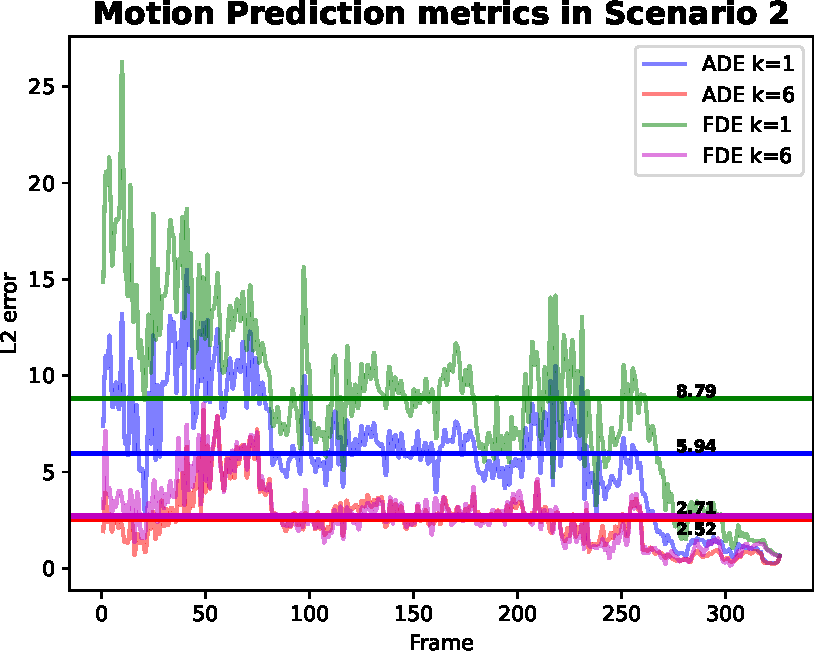
\includegraphics[width=0.9\textwidth]{chapter_8_Applications/scenarios/scenario_2/scenario_2_quantitative.pdf}
	\captionsetup{justification=justified}
	\caption[Scenario 2 quantitative results]{Scenario 2 quantitative results. Constant lines represent the mean value for the corresponding metric throughout the whole scenario.}
	\label{fig:chapter_8_Applications/scenarios/scenario_2/scenario_2_quantitative}
\end{figure}

\begin{figure}[]
	\begin{subfigure}{0.48\textwidth}
		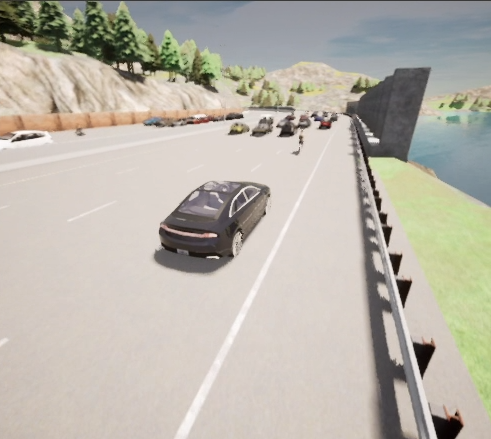
\includegraphics[width=\textwidth, trim={0 0 0 0.5cm},clip]{chapter_8_Applications/scenarios/scenario_2/scenario_2_highway_carla_t.png}
		\caption{\ac{CARLA} at frame $t$}
		\label{subfig:chapter_8_Applications/scenarios/scenario_2/scenario_2_highway_carla_t}
	\end{subfigure}
	%\hfill
	\begin{subfigure}{0.48\textwidth}
		\fbox{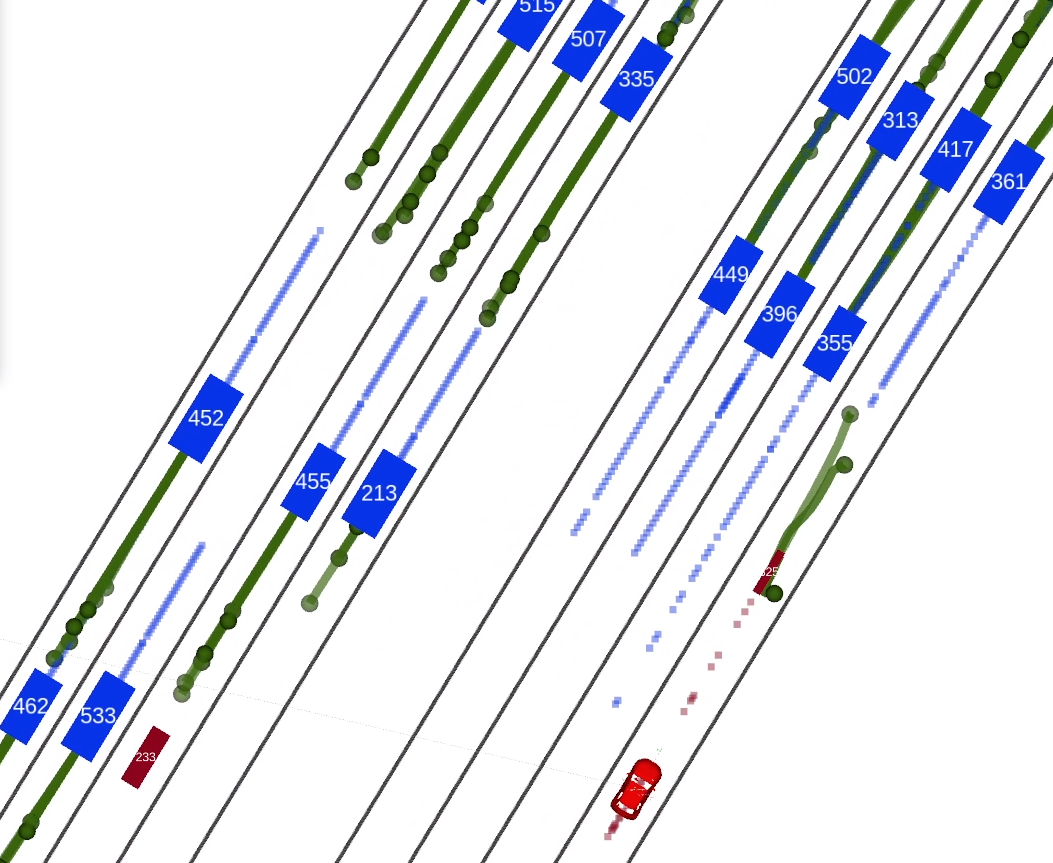
\includegraphics[width=\textwidth, trim={1.3cm 0 1cm 0},clip]{chapter_8_Applications/scenarios/scenario_2/scenario_2_highway_rviz_t.png}}
		\caption{\ac{RVIZ} at frame $t$}
		\label{subfig:chapter_8_Applications/scenarios/scenario_2/scenario_2_highway_rviz_t}
	\end{subfigure}
	\begin{subfigure}{0.48\textwidth}
		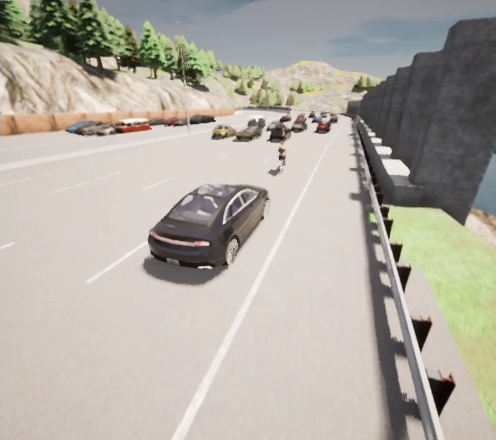
\includegraphics[width=\textwidth]{chapter_8_Applications/scenarios/scenario_2/scenario_2_highway_carla_t+15.png}
		\caption{\ac{CARLA} at frame $t+15$}
		\label{subfig:chapter_8_Applications/scenarios/scenario_2/scenario_2_highway_carla_t+15}
	\end{subfigure}
	%\hfill
	\begin{subfigure}{0.48\textwidth}
		\fbox{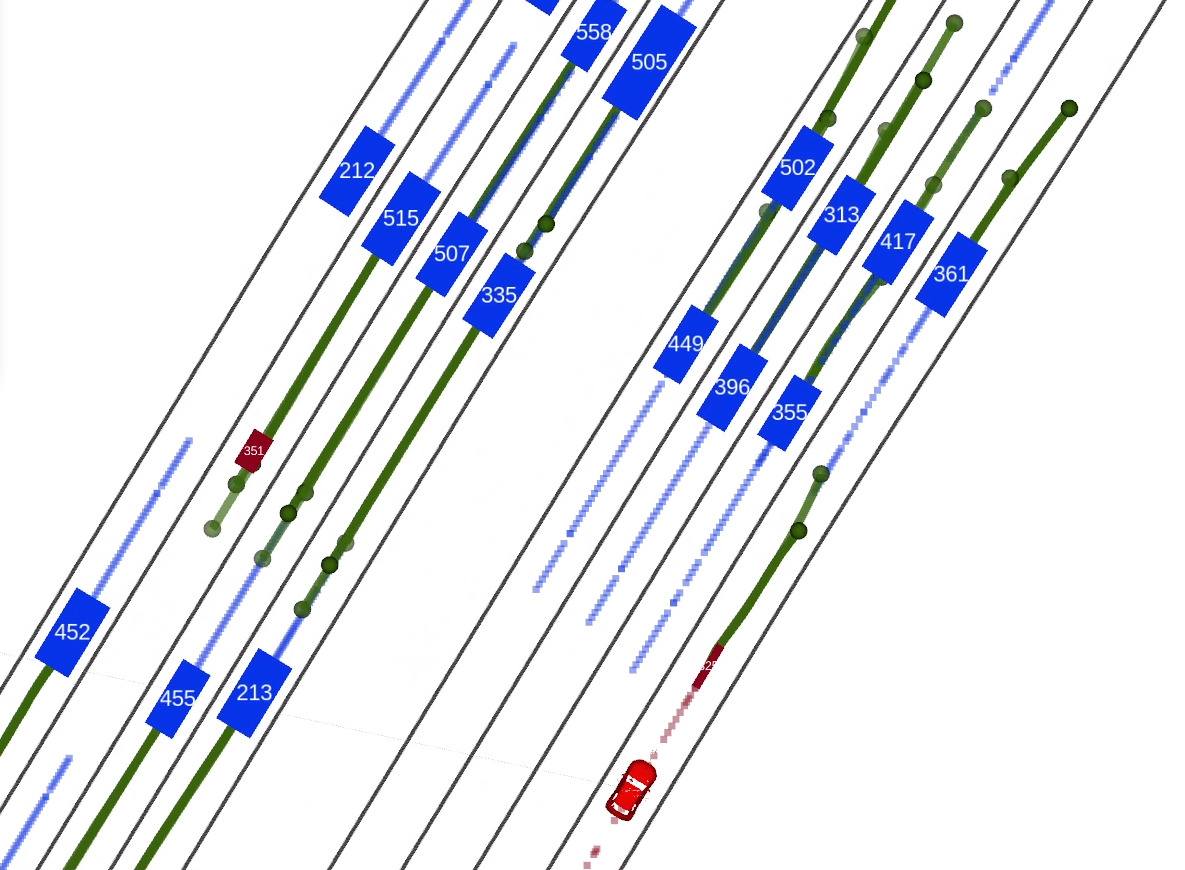
\includegraphics[width=\textwidth, trim={4cm 0 3cm 0},clip]{chapter_8_Applications/scenarios/scenario_2/scenario_2_highway_rviz_t+15.png}}
		\caption{\ac{RVIZ} at frame $t+15$}
		\label{subfig:chapter_8_Applications/scenarios/scenario_2/scenario_2_highway_rviz_t+15}
	\end{subfigure}
	\begin{subfigure}{0.48\textwidth}
		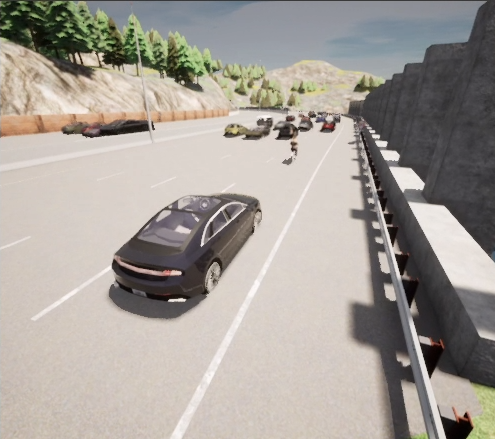
\includegraphics[width=\textwidth]{chapter_8_Applications/scenarios/scenario_2/scenario_2_highway_carla_t+30.png}
		\caption{\ac{CARLA} at frame $t+30$}
		\label{subfig:chapter_8_Applications/scenarios/scenario_2/scenario_2_highway_carla_t+30}
	\end{subfigure}
	\hfill
	\begin{subfigure}{0.48\textwidth}
		\fbox{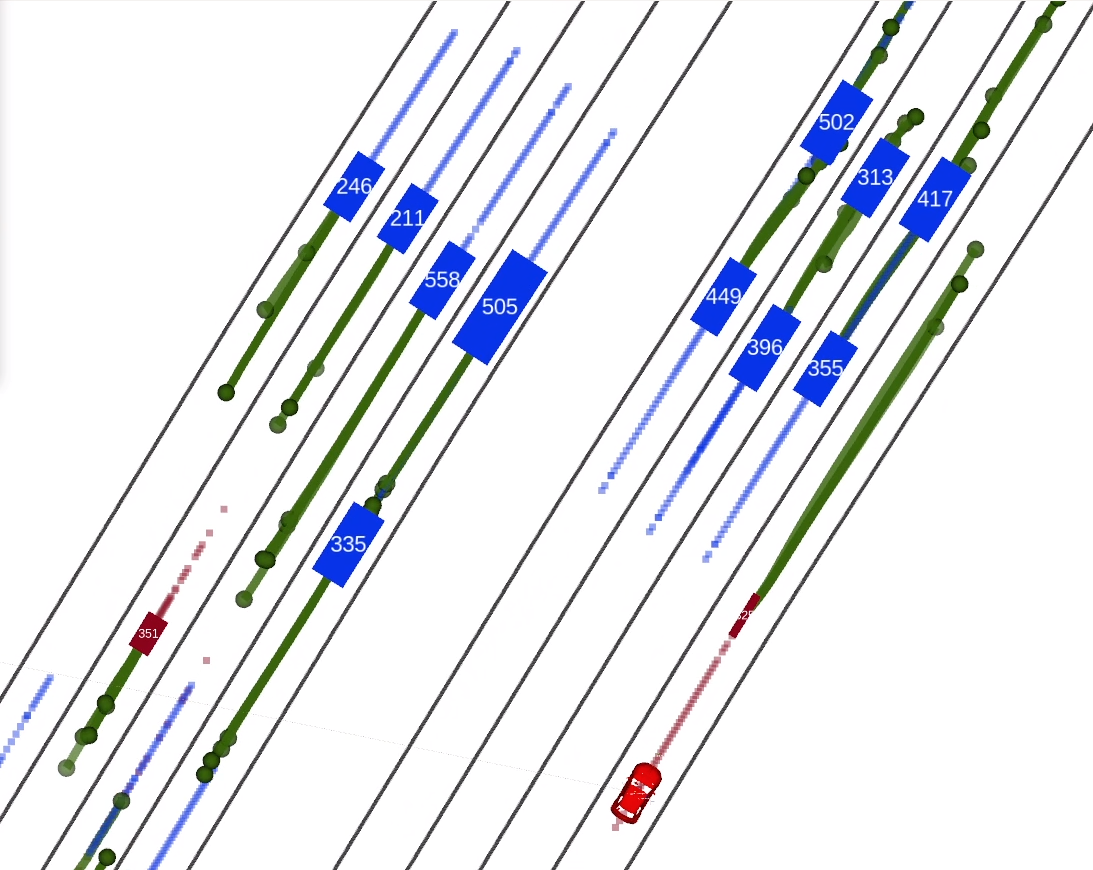
\includegraphics[width=\textwidth, trim={2cm 0 3cm 1cm},clip]{chapter_8_Applications/scenarios/scenario_2/scenario_2_highway_rviz_t+30.png}}
		\caption{\ac{RVIZ} at frame $t+30$}
		\label{subfig:chapter_8_Applications/scenarios/scenario_2/scenario_2_highway_rviz_t+30}
	\end{subfigure}
	%\captionsetup{justification=justified}
	\caption{Scenario 2 frames of interest}
	\label{fig:chapter_8_Applications/scenarios/scenario_2_frames_of_interest}
\end{figure}

% Scenario 3

\begin{figure}[]
	\centering
	\fbox{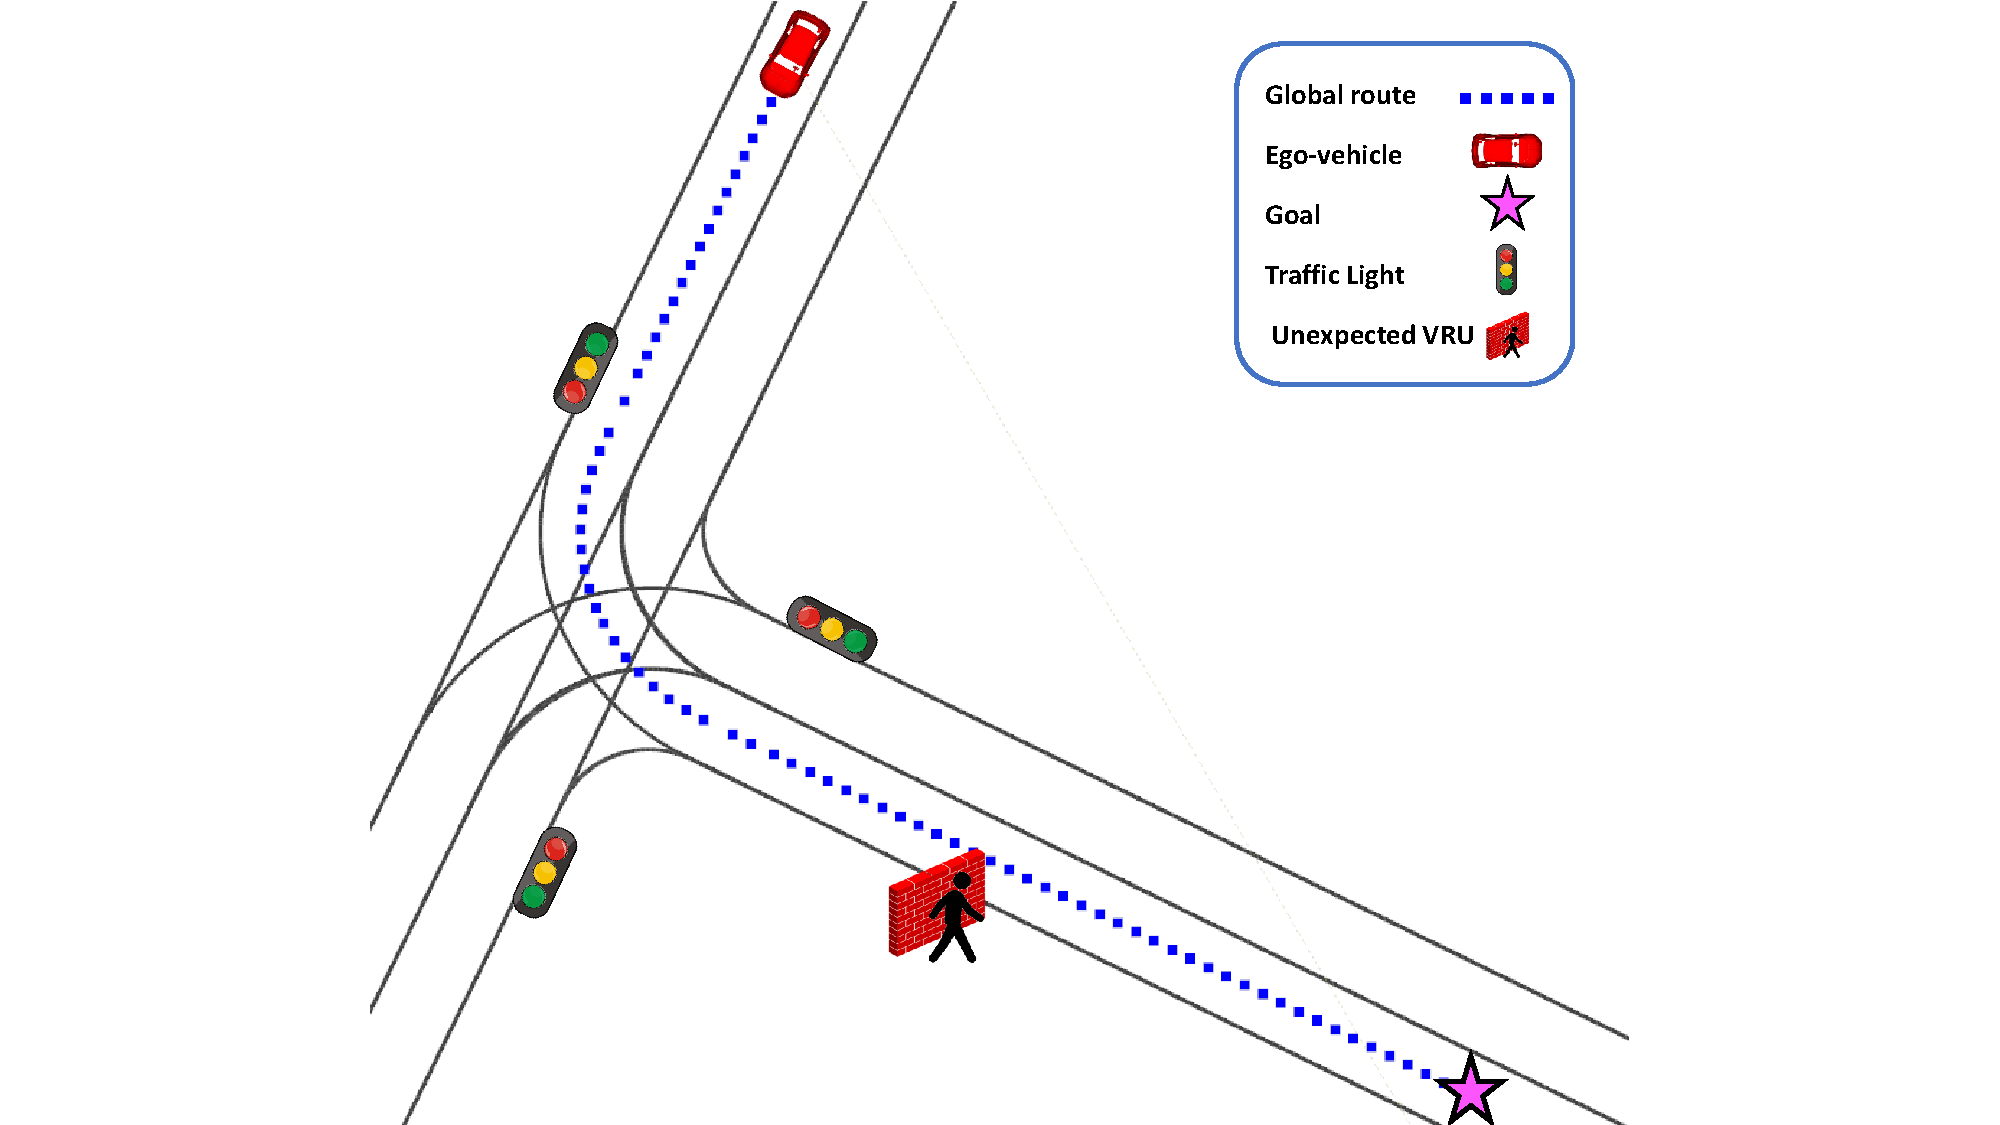
\includegraphics[width=0.9\textwidth, trim={4cm 0 4cm 0},clip]{chapter_8_Applications/scenarios/scenario_3/scenario_3_route1_town01_training.pdf}}
	%\captionsetup{justification=justified}
	\caption{Scenario 3 overview: Red Traffic Light and Unexpected \ac{VRU}}
	\label{fig:chapter_8_Applications/scenarios/scenario_3/scenario_3_route1_town01_training}
\end{figure}

\begin{figure}[]
	\centering
	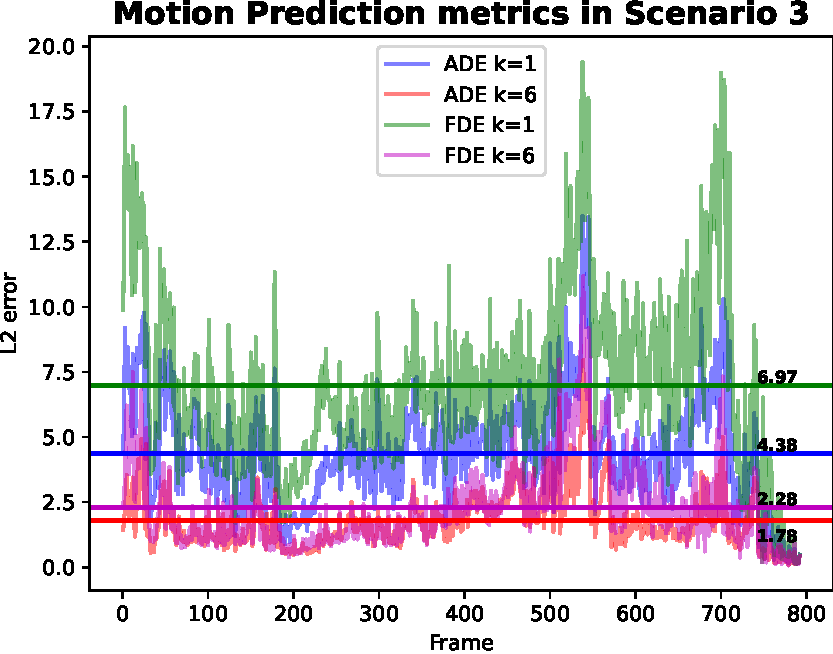
\includegraphics[width=0.9\textwidth]{chapter_8_Applications/scenarios/scenario_3/scenario_3_quantitative_threshold_3.pdf}
	\captionsetup{justification=justified}
	\caption[Scenario 3 quantitative results]{Scenario 3 quantitative results. Constant lines represent the mean value for the corresponding metric throughout the whole scenario.}
	\label{fig:chapter_8_Applications/scenarios/scenario_3/scenario_3_quantitative_threshold_3}
\end{figure}

\begin{figure}[]
	\begin{subfigure}{0.42\textwidth}
		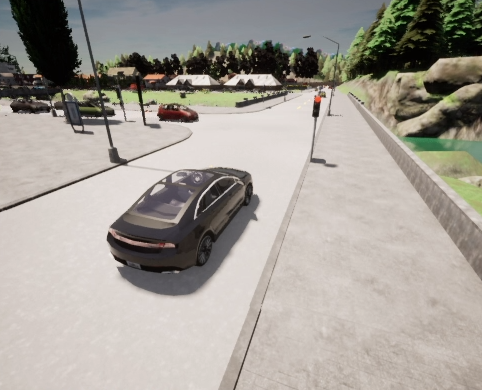
\includegraphics[width=\textwidth]{chapter_8_Applications/scenarios/scenario_3/scenario_3_rtl_carla_t.png}
		\caption{\ac{CARLA} at frame $t$}
		\label{subfig:chapter_8_Applications/scenarios/scenario_3/scenario_3_rtl_carla_t}
	\end{subfigure}
	%\hfill
	\begin{subfigure}{0.42\textwidth}
		\fbox{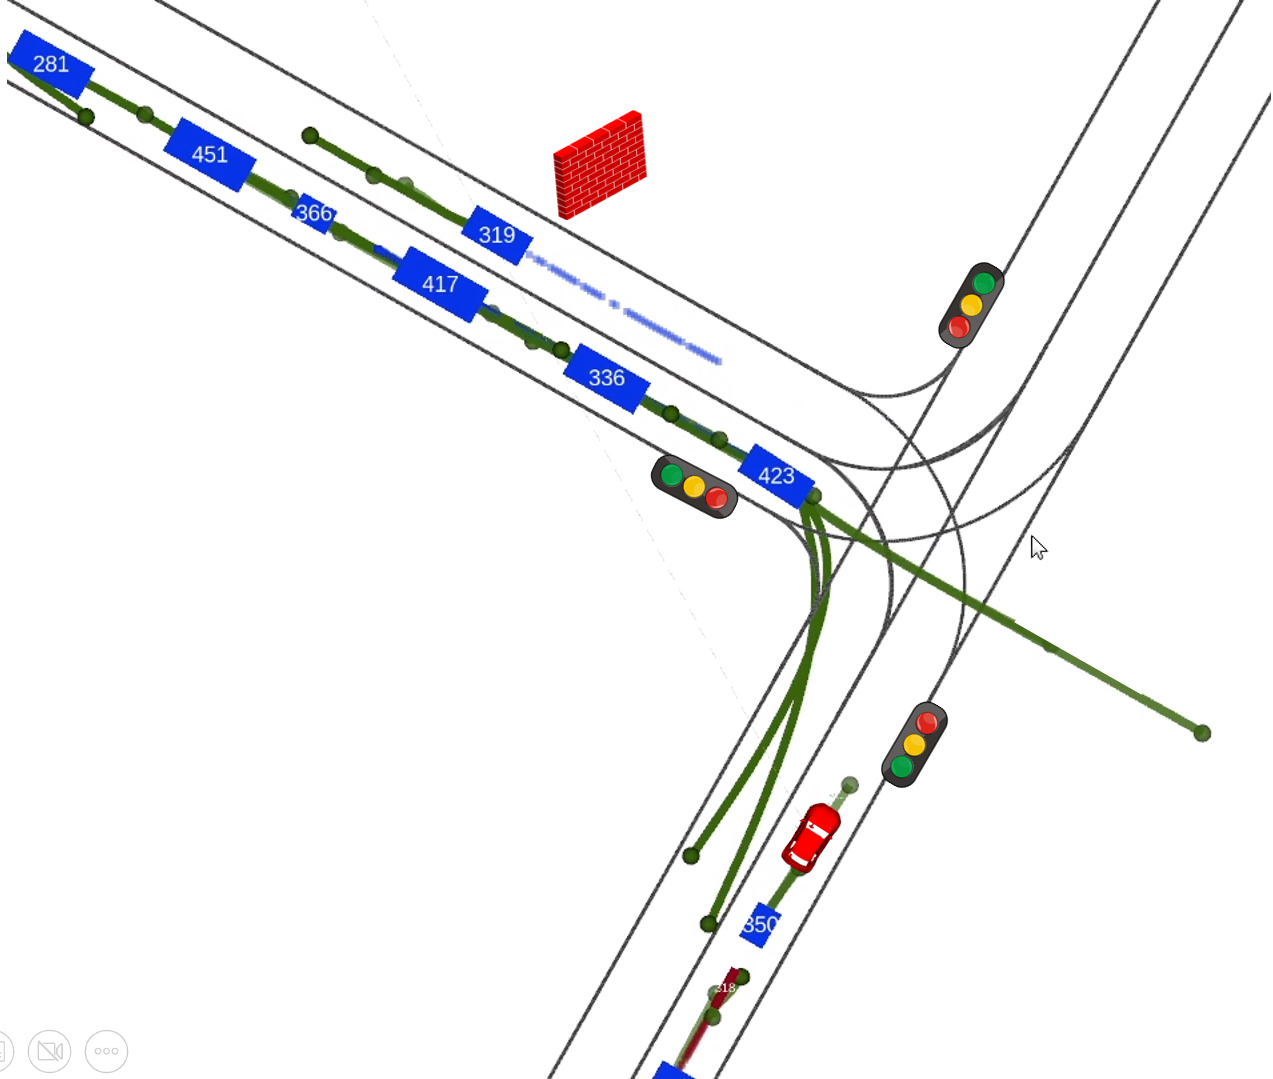
\includegraphics[width=\textwidth, trim={0 0 0 1cm},clip]{chapter_8_Applications/scenarios/scenario_3/scenario_3_rtl_rviz_t.png}}
		\caption{\ac{RVIZ} at frame $t$}
		\label{subfig:chapter_8_Applications/scenarios/scenario_3/scenario_3_rtl_rviz_t}
	\end{subfigure}
	\tabularnewline
	\begin{subfigure}{0.42\textwidth}
		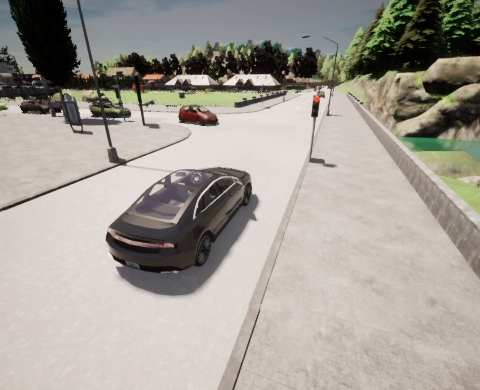
\includegraphics[width=\textwidth]{chapter_8_Applications/scenarios/scenario_3/scenario_3_rtl_carla_t+20.png}
		\caption{\ac{CARLA} at frame $t+5$}
		\label{subfig:chapter_8_Applications/scenarios/scenario_3/scenario_3_rtl_carla_t+20}
	\end{subfigure}
	%\hfill
	\begin{subfigure}{0.42\textwidth}
		\fbox{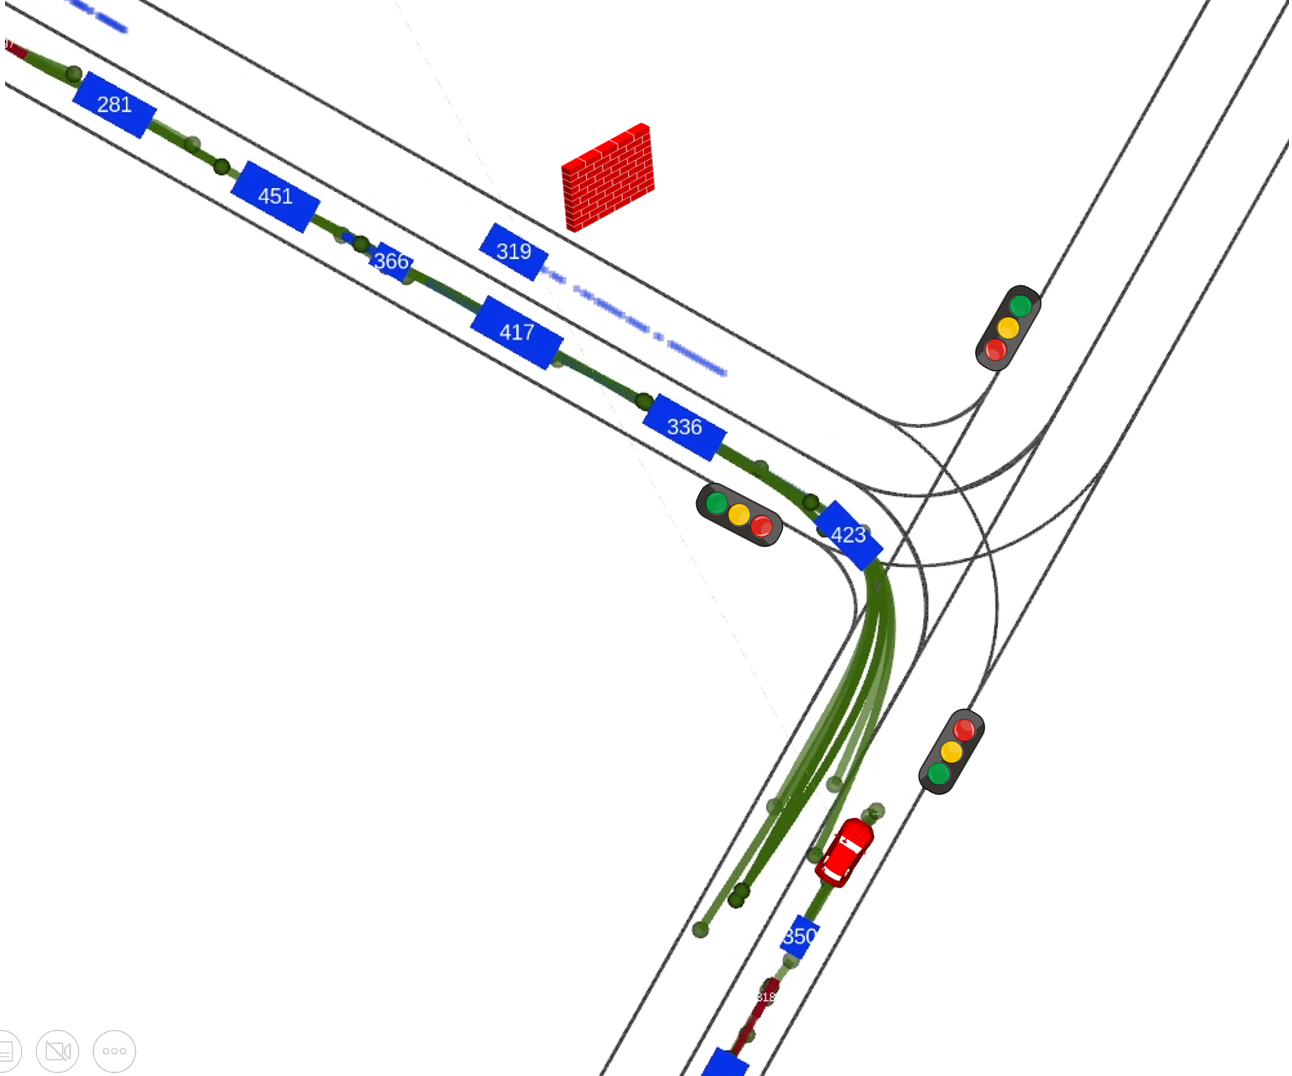
\includegraphics[width=\textwidth, trim={0 0 0 0.5cm},clip]{chapter_8_Applications/scenarios/scenario_3/scenario_3_rtl_rviz_t+20.png}}
		\caption{\ac{RVIZ} at frame $t+5$}
		\label{subfig:chapter_8_Applications/scenarios/scenario_3/scenario_3_rtl_rviz_t+20}
	\end{subfigure}
	\tabularnewline
	\begin{subfigure}{0.42\textwidth}
		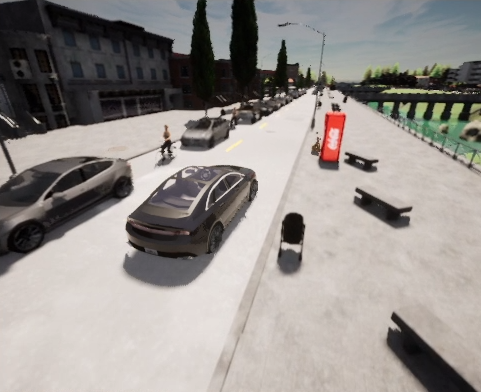
\includegraphics[width=\textwidth]{chapter_8_Applications/scenarios/scenario_3/scenario_3_VRU_carla_t.png}
		\caption{\ac{CARLA} at frame $t+145$}
		\label{subfig:chapter_8_Applications/scenarios/scenario_3/scenario_3_VRU_carla_t}
	\end{subfigure}
	%\hfill
	\begin{subfigure}{0.42\textwidth}
		\fbox{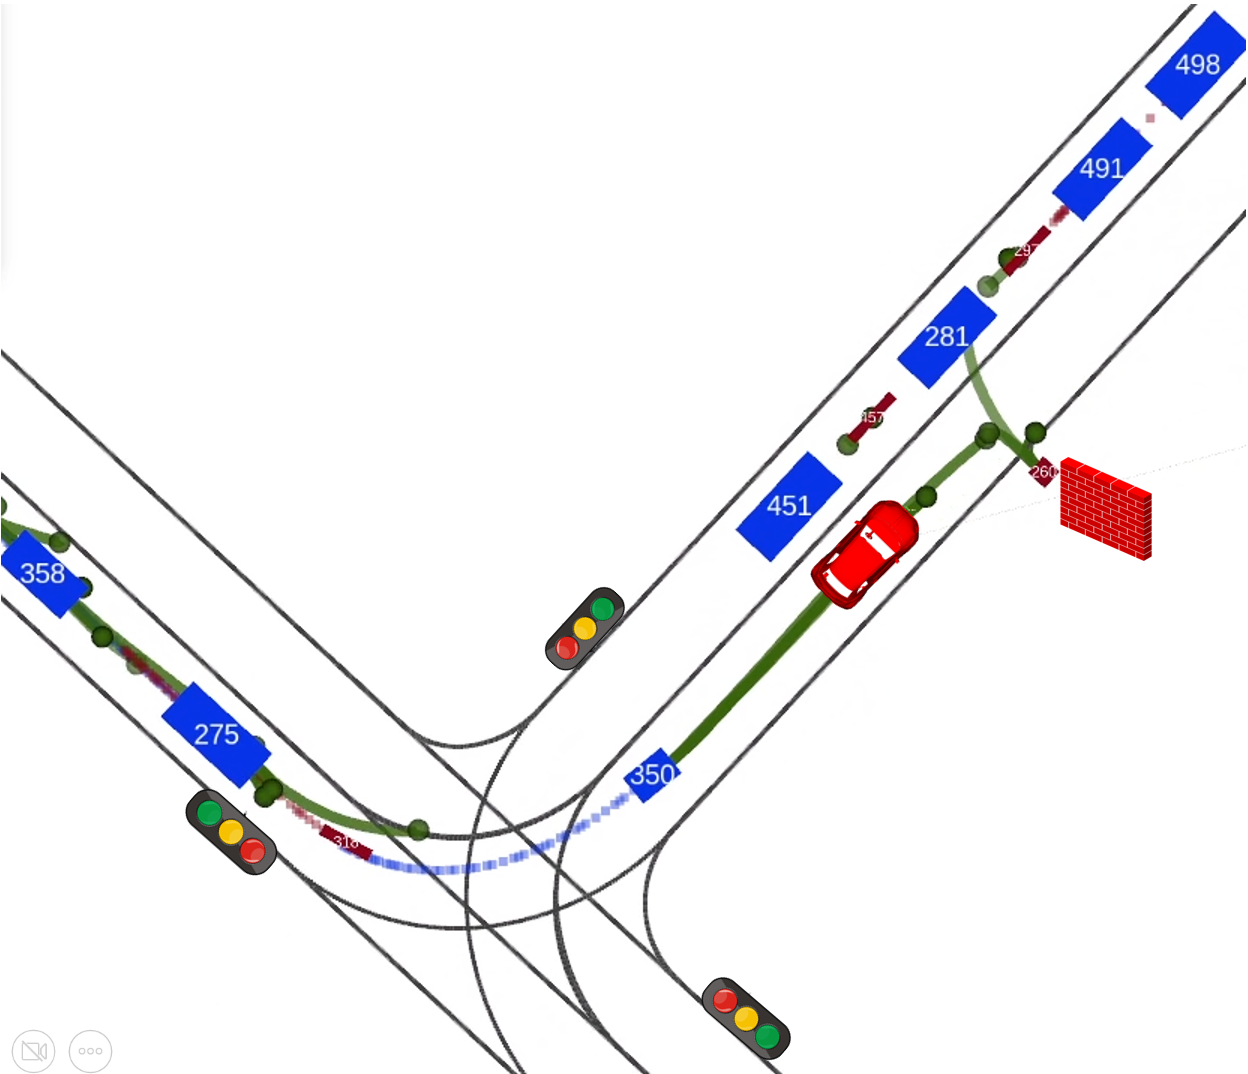
\includegraphics[width=\textwidth, trim={0 0 0 1cm},clip]{chapter_8_Applications/scenarios/scenario_3/scenario_3_VRU_rviz_t.png}}
		\caption{\ac{RVIZ} at frame $t+145$}
		\label{subfig:chapter_8_Applications/scenarios/scenario_3/scenario_3_VRU_rviz_t}
	\end{subfigure}
	\tabularnewline
	\begin{subfigure}{0.42\textwidth}
		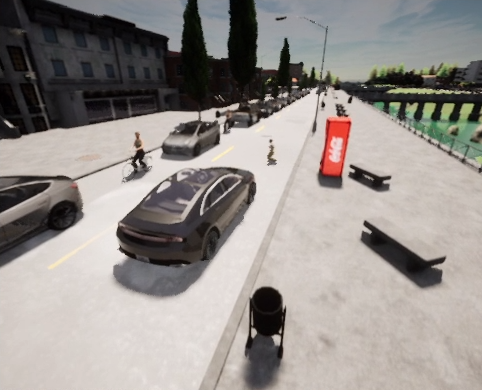
\includegraphics[width=\textwidth]{chapter_8_Applications/scenarios/scenario_3/scenario_3_VRU_carla_t+5.png}
		\caption{\ac{CARLA} at frame $t+147$}
		\label{subfig:chapter_8_Applications/scenarios/scenario_3/scenario_3_VRU_carla_t+5}
	\end{subfigure}
	\hfill
	\begin{subfigure}{0.42\textwidth}
		\fbox{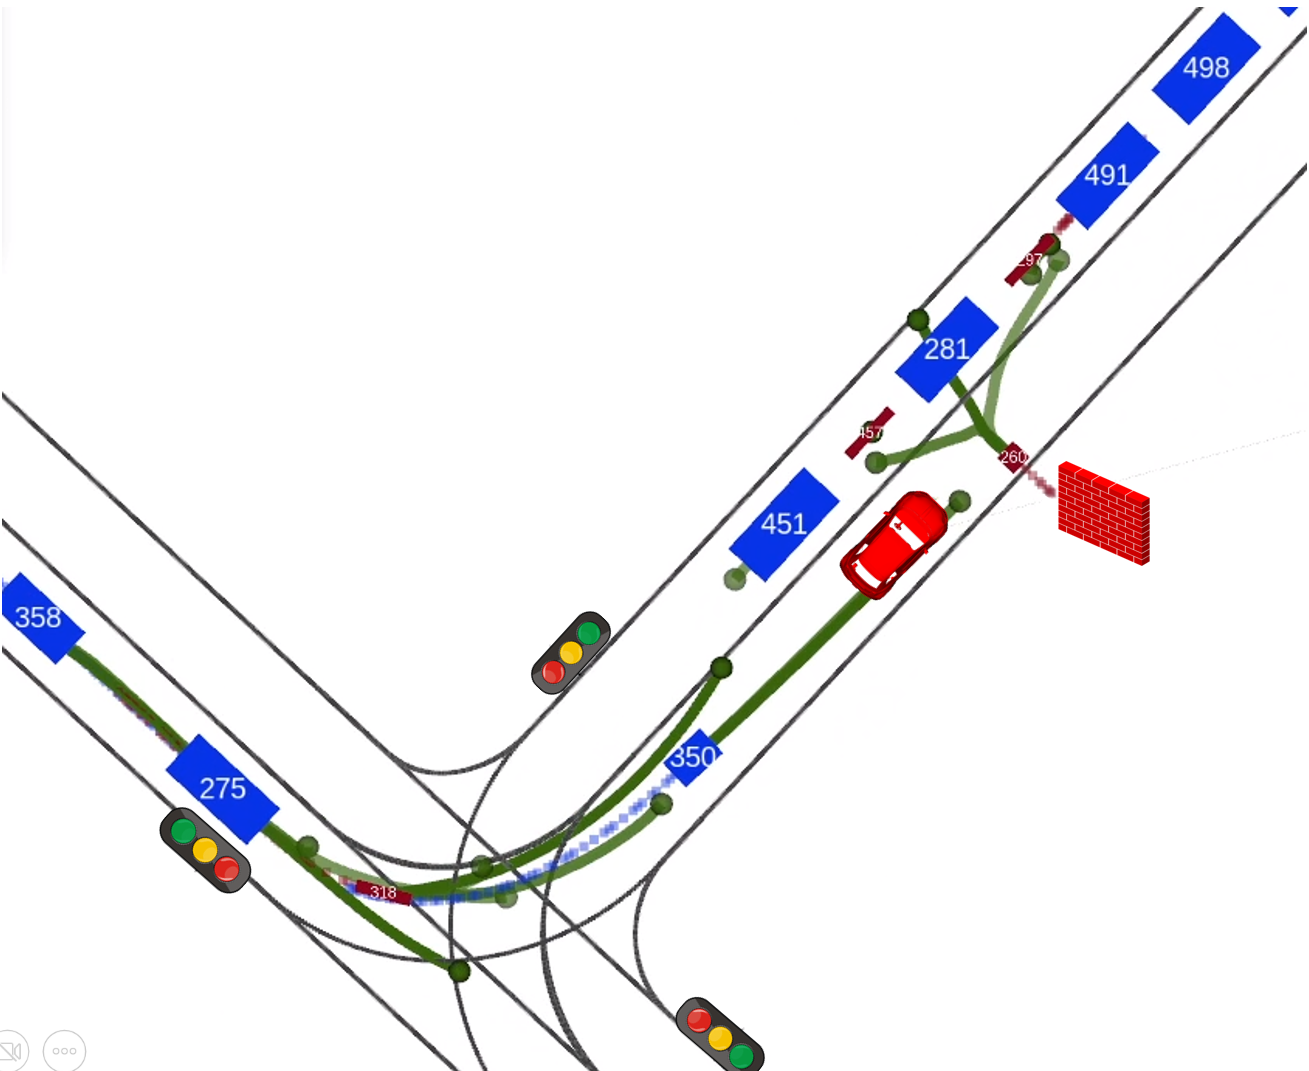
\includegraphics[width=\textwidth]{chapter_8_Applications/scenarios/scenario_3/scenario_3_VRU_rviz_t+5.png}}
		\caption{\ac{RVIZ} at frame $t+147$}
		\label{subfig:chapter_8_Applications/scenarios/scenario_3/scenario_3_VRU_rviz_t+5}
	\end{subfigure}
	%\captionsetup{justification=justified}
	\caption{Scenario 3 frames of interest}
	\label{fig:chapter_8_Applications/scenarios/scenario_3_frames_of_interest}
\end{figure}

% Scenario 4

\begin{figure}[]
	\centering
	\fbox{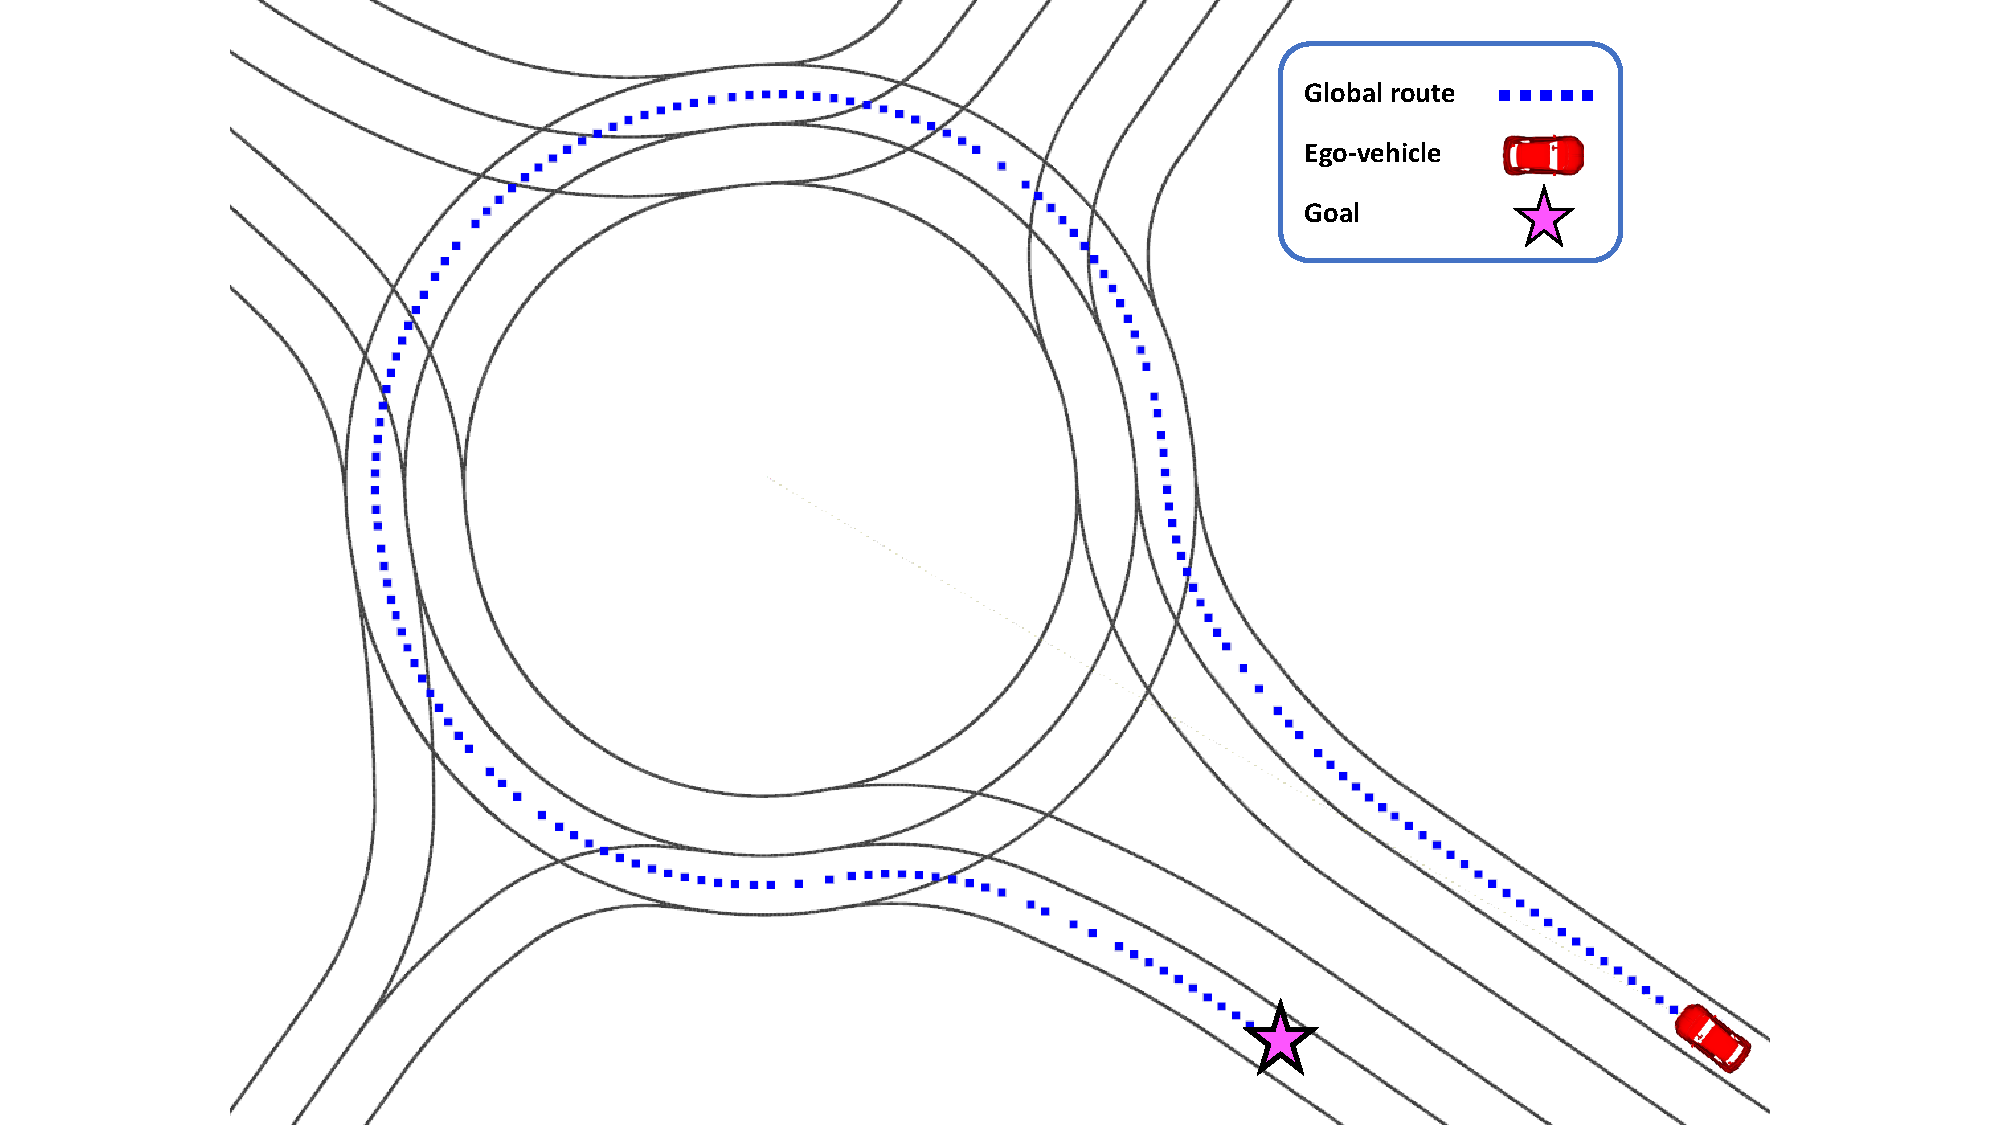
\includegraphics[width=0.9\textwidth, trim={3cm 0 3cm 0},clip]{chapter_8_Applications/scenarios/scenario_4/scenario_4_route_27_town03_training.pdf}}
	%\captionsetup{justification=justified}
	\caption{Scenario 4 overview: Crowded roundabout}
	\label{fig:chapter_8_Applications/scenarios/scenario_4/scenario_4_route_27_town03_training}
\end{figure}

\begin{figure}[]
	\centering
	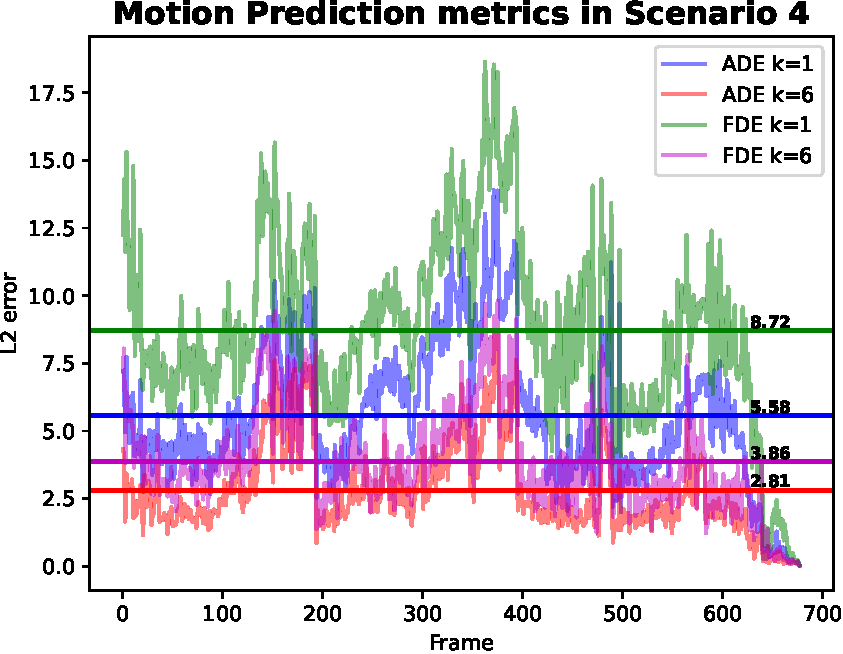
\includegraphics[width=0.9\textwidth]{chapter_8_Applications/scenarios/scenario_4/scenario_4_quantitative.pdf}
	\captionsetup{justification=justified}
	\caption[Scenario 4 quantitative results]{Scenario 4 quantitative results. Constant lines represent the mean value for the corresponding metric throughout the whole scenario.}
	\label{fig:chapter_8_Applications/scenarios/scenario_4/scenario_4_quantitative}
\end{figure}

\begin{figure}[t!]
	\begin{subfigure}{0.48\textwidth}
		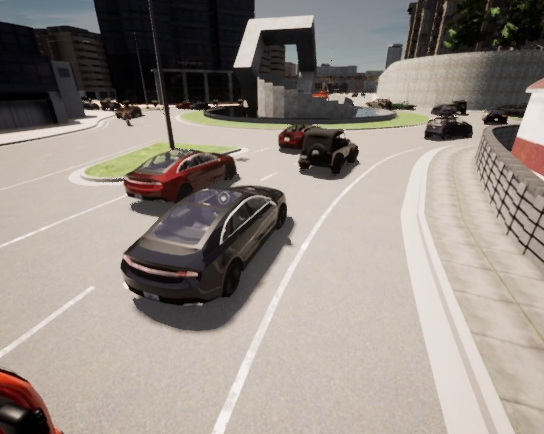
\includegraphics[width=\textwidth]{chapter_8_Applications/scenarios/scenario_4/scenario_4_roundabout_carla_t.png}
		\caption{\ac{CARLA} at frame $t$}
		\label{subfig:chapter_8_Applications/scenarios/scenario_4/scenario_4_roundabout_carla_t.png}
	\end{subfigure}
	\hfill 
	\begin{subfigure}{0.48\textwidth}
		\fbox{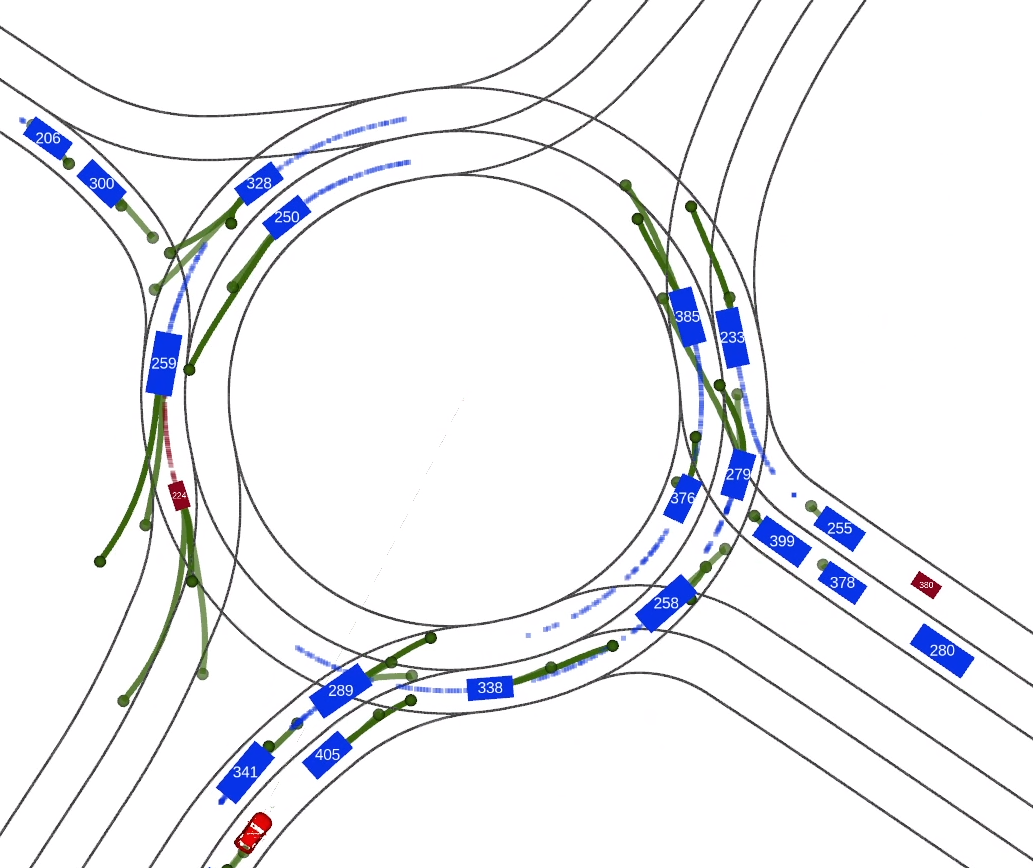
\includegraphics[width=\textwidth, trim={0 0 0 2cm},clip]{chapter_8_Applications/scenarios/scenario_4/scenario_4_roundabout_rviz_t.png}}
		\caption{\ac{RVIZ} at frame $t$}
		\label{subfig:chapter_8_Applications/scenarios/scenario_4/scenario_4_roundabout_rviz_t}
	\end{subfigure}
	\tabularnewline
	\begin{subfigure}{0.48\textwidth}
		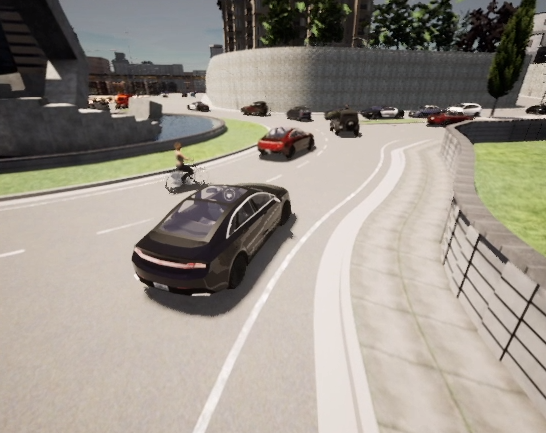
\includegraphics[width=\textwidth]{chapter_8_Applications/scenarios/scenario_4/scenario_4_roundabout_carla_t+40.png}
		\caption{\ac{CARLA} at frame $t+40$}
		\label{subfig:chapter_8_Applications/scenarios/scenario_4/scenario_4_roundabout_carla_t+40.png}
	\end{subfigure}
	\hfill 
	\begin{subfigure}{0.48\textwidth}
		\fbox{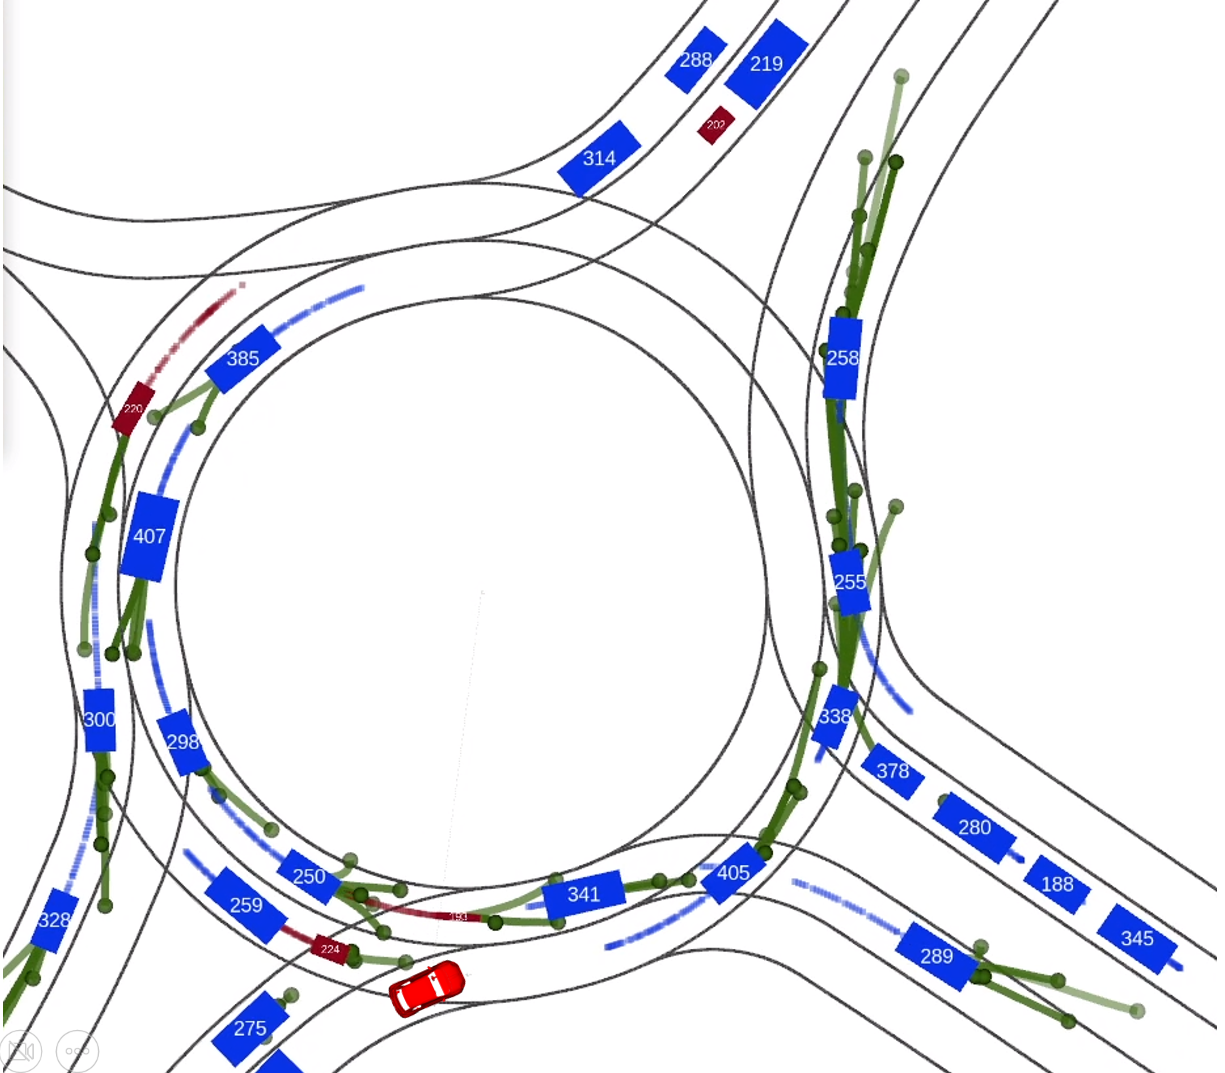
\includegraphics[width=\textwidth, trim={0 1cm 0 1cm},clip]{chapter_8_Applications/scenarios/scenario_4/scenario_4_roundabout_rviz_t+40.png}}
		\caption{\ac{RVIZ} at frame $t+40$}
		\label{subfig:chapter_8_Applications/scenarios/scenario_4/scenario_4_roundabout_rviz_t+40}
	\end{subfigure}
	\tabularnewline
	\begin{subfigure}{0.48\textwidth}
		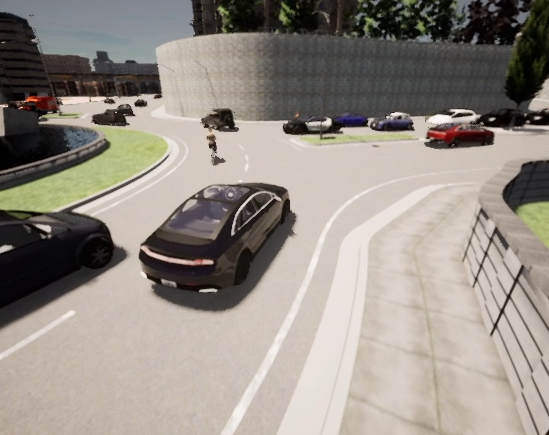
\includegraphics[width=\textwidth]{chapter_8_Applications/scenarios/scenario_4/scenario_4_roundabout_carla_t+80.png}
		\caption{\ac{CARLA} at frame $t+80$}
		\label{subfig:chapter_8_Applications/scenarios/scenario_4/scenario_4_roundabout_carla_t+80}
	\end{subfigure}
	\hfill
	\begin{subfigure}{0.48\textwidth}
		\fbox{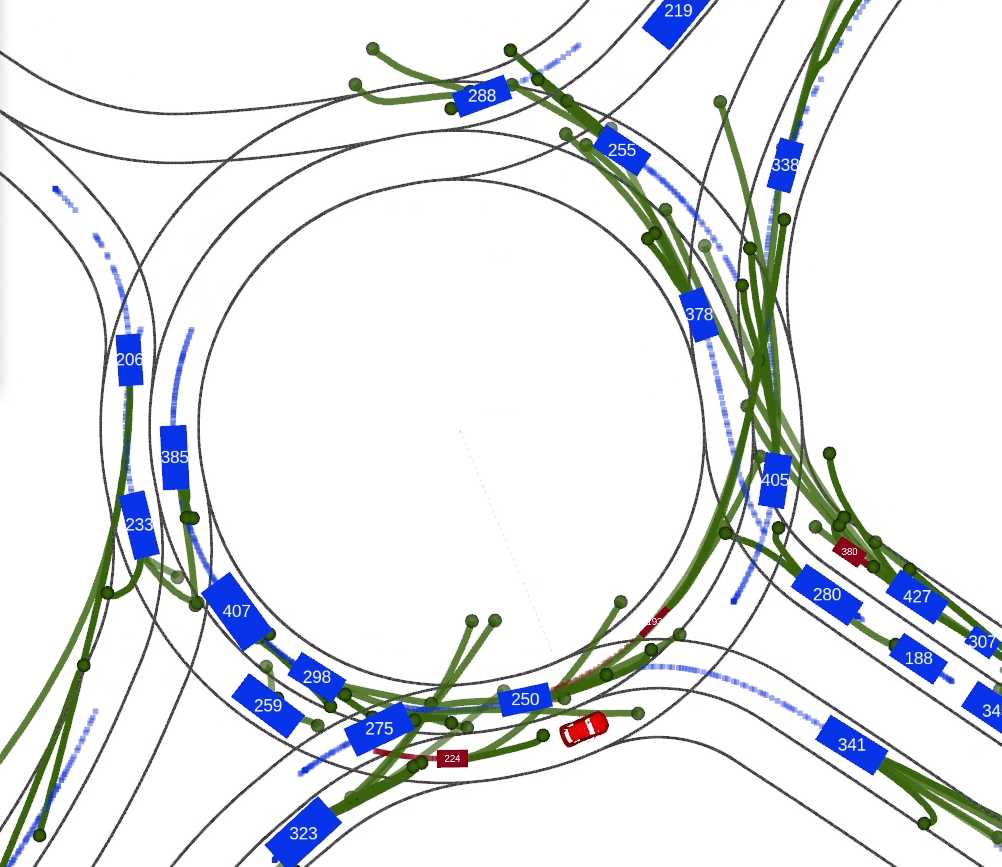
\includegraphics[width=\textwidth, trim={0 0.5 0 2.5cm},clip]{chapter_8_Applications/scenarios/scenario_4/scenario_4_roundabout_rviz_t+80.png}}
		\caption{\ac{RVIZ} at frame $t+80$}
		\label{subfig:chapter_8_Applications/scenarios/scenario_4/scenario_4_roundabout_rviz_t+80}
	\end{subfigure}
	\tabularnewline
	%\captionsetup{justification=justified}
	\caption{Scenario 4 frames of interest}
	\label{fig:chapter_8_Applications/scenarios/scenario_4_frames_of_interest}
\end{figure}